\documentclass[runningheads,envcountsame,envcountsect,orivec]{llncs}
\usepackage[letterpaper,margin=25mm,headheight=12pt,headsep=8mm]{geometry}
\usepackage[T1]{fontenc}
\usepackage[english]{babel}
\usepackage{amsmath,mathtools}
\usepackage{amssymb}
\usepackage{booktabs,tabularx,array}
\usepackage{tikz,placeins,needspace}
\definecolor{bkwink}{HTML}{25314A}
\definecolor{bkwmuted}{HTML}{5A6578}
\definecolor{bkwblue}{HTML}{315D88}
\definecolor{bkworange}{HTML}{AB501E}
\definecolor{bkwline}{HTML}{D7DFE8}
\definecolor{bkwshrink}{HTML}{4E397A}
\definecolor{bkwneutral}{HTML}{F0ECE4}
\usepackage[hidelinks]{hyperref}
\hypersetup{pdftitle={Faster Classical and Quantum BKW for LWE},
             pdfsubject={Algorithms for learning with errors},
             pdfkeywords={Learning with errors, BKW, lattice cryptanalysis, quantum algorithms},
             pdfauthor={}}
\urlstyle{same}
\setlength{\emergencystretch}{2em}
\newcommand{\E}{\mathbb E}
\spnewtheorem{model}[theorem]{Model}{\bfseries}{\rmfamily}
\title{Faster Classical and Quantum BKW for LWE}
\titlerunning{Faster Classical and Quantum BKW for LWE}
\author{Samuel J. Adams \and Luis Iglesias}
\authorrunning{Author}
\institute{PQProtect Inc., USA \\\texttt{samuel.j.adams80@gmail.com}\\ \texttt{luisiglesias.vigo@outlook.com}}
\begin{document}
\maketitle

\begin{abstract}
We improve classical and quantum BKW for learning with errors at Regev's parameters. Each coded round sets a separate radius limit for each earlier coordinate block. A tighter limit in a later round allows wider rounding bins when the block first enters, but makes suitable pairs harder to find. Choosing these limits together with the block sizes gives classical time $2^{0.8883n+o(n)}$ and quantum time $2^{0.8737n+o(n)}$ with Grover search. Reusing a quantum-walk state to find many pairs lowers the time to $2^{0.8643n+o(n)}$. These algorithms read fresh classical samples. From only $\Theta(n\log n)$ original samples, amplification gives classical time $2^{1.6359n+o(n)}$, quantum time $2^{1.6130n+o(n)}$ with Grover search, and $2^{1.5979n+o(n)}$ with reusable walks. Integral equations define the constants in these bounds. The running times are heuristic: we assume that the intermediate lists have the distance and filter statistics of independent random directions within each block. The walk also needs these statistics inside its filters and coherent reads and writes of working memory.
\keywords{Learning With Errors \and BKW \and Lattice Cryptanalysis \and Quantum Algorithms}
\end{abstract}


\section{Introduction}

Learning with errors (LWE) asks us to recover a secret from
noisy linear equations modulo an integer. Regev connected its
hardness to worst-case lattice problems~\cite{Regev09}.
The cost of an attack depends on the dimension, modulus, error
size, and number of available equations, called samples.

The Blum--Kalai--Wasserman (BKW) algorithm subtracts pairs of
samples that agree on a block of
coordinates~\cite{BKW03,ACFFP15}. Each subtraction cancels that
block and adds noise. Repeating this operation reduces the
dimension until the remaining bias can be detected. Coded BKW
allows a small difference on the new block and uses sieving to
control the residuals on earlier blocks.

\subsection{Related Work}
\label{sec:related-regev}

BKW was introduced for learning parity with noise. Extensions
to LWE use lazy modulus switching and coded BKW to reduce the
cost of grouping samples~\cite{ACFFP15,AFFP14,GJS15,KF15,HKM18}.
Guo et al.\ combined coded BKW with classical and quantum lattice
sieving~\cite{GJMS17,GJMS19}. M{\aa}rtensson varied the radius
factor between rounds, while applying the same factor to all
earlier coordinates within a round~\cite{M19}.
Guo et al.\ also proposed optimizing the coordinate sets and
reduction factors of individual sieving operations, and left
the resulting general optimization open~\cite[Section~VIII-F]{GJMS19}.
Here we choose separate block radii jointly with the block sizes.

Other attacks use BKZ with enumeration or sieving
\cite{APS15,BDGL16}. Earlier comparisons at Regev's
parameter scales favor BKW when many samples are
available~\cite[Section~6.3]{GJMS17}, \cite[Section~VI]{M19}.
With fewer samples, amplification generates more equations by
combining the originals, at the cost of larger errors
\cite[Section~7.3]{HKM18}. Concrete BKW costs and time--memory
tradeoffs have also been refined~\cite{BGJMW21,WBLW25}.
Distribution bounds for Wagner-style SIS algorithms explain
why a fully rigorous LWE analysis remains
difficult~\cite[Section~4.3]{DEL25}.

Cao, Cheng and Weng study quantum BKW with exact multiway
cancellations~\cite{CCW24}. Their Algorithm~6 searches over an
intermediate target. Its Regev cost must include that search
as well as the inner searches priced before their Lemma~7;
we therefore omit that formula from the comparison tables.
Here all reductions subtract pairs, and we include both the
Grover or walk search and the construction of its working lists.

\subsection{Contributions}
\label{sec:contributions}

We choose a separate radius factor for each earlier block in
every round, jointly with the block sizes. We carry out this
optimization for classical search, Grover search, and reusable
quantum walks. The walks use established filtering and pair-reporting
methods for lattice sieving and multiple-collision search; their
costs lead to different BKW radii and block sizes. Finally, amplification applies all three
algorithms to $\Theta(n\log n)$ original samples.
The bounds assume the list statistics in
Models~\ref{def:model} and~\ref{def:quantum-model}.

We consider search-LWE in dimension $n$ with prime
$q=\Theta(n^2)$ and independent errors of scale
\begin{align}
 \sigma=\frac{q}{\sqrt{2\pi n}\,(\log_2 n)^2}.
 \label{eq:regev}
\end{align}
These are the Regev parameter scales used in the BKW
comparisons \cite{Regev09}, \cite{GJMS19} and \cite{M19}. A fresh sample is
an independent draw with the same secret. We allow
exponentially many fresh classical samples and charge
every sample read.


All three variants use the same formula for the time exponent.
Let $N(x)\,dx$ count the coordinates assigned to coded
rounds indexed by $[x,x+dx]$, in the units of
Section~\ref{sec:shared-schedule}. Let $X$ mark the end of those
rounds, and let $O(x)$ be the additional
cost exponent for the pair search in round $x$. The numerator
below accounts for carrying enough rows to supply later rounds.
The denominator counts the coordinates handled per unit of
the normalized budget.
\begin{align}
 a
 &=\frac{1+\displaystyle\max_{1\le x\le y\le X}\bigl(O(x)-O(y)\bigr)}
         {1+\displaystyle\int_1^X(1-3x/4)N(x)\,dx}.
 \label{eq:main-exponent}
\end{align}
Section~\ref{sec:shared-schedule} defines the common equations
for $N$ and $X$. The variants differ in the pair search
and the resulting costs.
The classical, Grover, and walk variants use the cost functions of
Lemmas~\ref{lem:local}, \ref{lem:grover-local}, and \ref{lem:q-radius},
respectively, with the corresponding overheads
\eqref{eq:c-overhead}, \eqref{eq:grover-overhead}, and \eqref{eq:q-overhead}.
Solving these equations up to the endpoint
\eqref{eq:shared-endpoint} defines the coefficients below;
the decimals are numerical evaluations. We optimize each round's
radius choices, without claiming the best possible BKW schedule.

\begin{theorem}[Classical BKW for Regev LWE]
\label{thm:classical}
Let $q=\Theta(n^2)$ be prime and let the errors have the scale
in \eqref{eq:regev}, with either Gaussian law of
Section~\ref{sec:prelim}. Under Model~\ref{def:model}, a
randomized classical algorithm recovers the secret with
probability $1-o(1)$ in time $2^{a_{\rm C}n+o(n)}$ and uses
at most as many fresh samples and stored words.
This gives
\begin{align}
 a_{\rm C}=0.88825\ldots .
 \label{eq:c-main}
\end{align}
\end{theorem}

\begin{samepage}
\begin{theorem}[Quantum BKW with Grover search]
\label{thm:quantum-grover}
Let the input parameters and error law be as in
Theorem~\ref{thm:classical}. Assume Model~\ref{def:model} and
coherent indexed reads of classically constructed tables at
polynomial cost per operation. A quantum algorithm recovers
the secret with probability $1-o(1)$ in time
$2^{a_{\rm G}n+o(n)}$ and uses at most as many fresh classical
samples and stored words.
This gives
\begin{align}
 a_{\rm G}=0.87367\ldots .
 \label{eq:grover-main}
\end{align}
\end{theorem}
\end{samepage}

\begin{theorem}[Quantum BKW with a reusable walk]
\label{thm:quantum}
Let the input parameters and error law be as in
Theorem~\ref{thm:classical}. Under Models~\ref{def:model}
and~\ref{def:quantum-model}, a quantum algorithm recovers
the secret with probability $1-o(1)$ in time
$2^{a_{\rm Q}n+o(n)}$ and uses at most as many fresh classical
samples and stored words.
This gives
\begin{align}
 a_{\rm Q}=0.86426\ldots .
 \label{eq:q-main}
\end{align}
\end{theorem}

Theorem~\ref{thm:quantum-grover} applies the separate-radius
optimization with the Grover search used in earlier BKW
analyses~\cite{GJMS19,M19,Laa16}. Theorem~\ref{thm:quantum}
also changes the pair-reporting method. This separates the
gains from block scheduling and from the quantum search.

\begin{corollary}[BKW from $\Theta(n\log n)$ original samples]
\label{cor:amplified-regev}
Let the parameters and error law be as in Theorem~\ref{thm:classical},
with only $\Theta(n\log n)$ independent original observations.
Under the respective list and memory assumptions of
Theorems~\ref{thm:classical}--\ref{thm:quantum}, the three algorithms
recover the secret with probability $1-o(1)$ in times
$2^{a_{\rm amp}n+o(n)}$, where
\begin{align*}
 a_{{\rm C},{\rm amp}}&=1.63588\ldots,&
 a_{{\rm G},{\rm amp}}&=1.61298\ldots,&
 a_{{\rm Q},{\rm amp}}&=1.59787\ldots.
\end{align*}
Use the same coordinate and search-cost functions in
formula~\eqref{eq:main-exponent},
replacing the initial $1$ in its denominator by $1/2$ and choosing
the largest $X\le4/3$ with $\tfrac32\int_1^XxN(x)\,dx\le1$.
The working lists are generated from the original observations;
their generation is included in the stated time.
\end{corollary}

\begin{proof}[Sketch]
Independently chosen bounded-coefficient combinations amplify the observations.
Conditional on the original errors, a collision bound makes the public
vectors negligibly close to uniform independently of the error residues,
with negligible loss for the whole list. The scalar Fourier bias permits one unit
of round depth, giving the changed denominator. Random column signs
and subexponential guessing on large residual coordinates give a
final test despite reuse of the pivot errors.
Appendix~\ref{app:amplification} proves these steps without an
additional sample-independence assumption.
\qed
\end{proof}

All algorithms use at most $2^{an+o(n)}$ stored words.
Grover search needs coherent reads of classical tables; the walk
also uses a coherently writable subset, quantified separately
in Section~\ref{app:evaluation}.

\paragraph{Time and original samples at the Regev scales.}
Tables~\ref{tab:classical-history} and~\ref{tab:quantum-history}
give leading time coefficients in $2^{an+o(n)}$. The sample
column counts independent input equations, including any pivots.
The cited BKW rows with limited original data include the cost
of generating their working lists. The three theorems concern fresh samples; Corollary~\ref{cor:amplified-regev}
uses only $\Theta(n\log n)$ original observations. The BKW estimates use the list assumptions
discussed in Section~\ref{sec:assumption-comparison}.

\begin{table}[!t]
\centering\small
\caption{Classical time coefficients for Regev LWE, grouped by
original sample count and ordered by decreasing $a$ within each group.
Bold rows are results of this paper. The dual rows use the sieve
cost of~\cite{BDGL16}; the benchmark models are described in
Section~\ref{sec:lattice-benchmarks}.}
\label{tab:classical-history}
\begin{tabularx}{\linewidth}{@{}>{\raggedright\arraybackslash}X>{\raggedright\arraybackslash}p{2.65cm}r@{}}
\toprule
Method & \shortstack[l]{Original LWE\\samples} & Coefficient $a$ \\
\midrule
\multicolumn{3}{@{}l}{\textit{$2^{\Theta(n)}$ samples}} \\
Dual BKZ benchmark~\cite[Section~6]{HKM18}
  & $2^{\Theta(n)}$ & $1.1699$ \\
Exact block elimination~\cite{ACFFP15,HKM18}
  & $2^{\Theta(n)}$ (fresh) & $1.0000$ \\
Progressive quantization (BKW2)~\cite{GJS15,KF15,HKM18}
  & $2^{\Theta(n)}$ (fresh) & $0.9299$ \\
Coded sieving with an exact prefix~\cite[Table~1]{GJMS17}
  & $2^{\Theta(n)}$ (fresh) & $0.8951$ \\
Optimized common factor~\cite[Table~III]{GJMS19}
  & $2^{\Theta(n)}$ (fresh) & $0.8927$ \\
Arithmetic progression~\cite[Table~I]{M19}
  & $2^{\Theta(n)}$ (fresh) & $0.8917$ \\
\textbf{\boldmath Separate block radii (Theorem~\ref{thm:classical})}
  & \textbf{\boldmath $2^{\Theta(n)}$ (fresh)} & $\boldsymbol{0.88825\ldots}$ \\
\midrule
\multicolumn{3}{@{}l}{\textit{$\Theta(n\log n)$ samples}} \\
Dual BKZ benchmark~\cite[Section~6]{HKM18}
  & $\Theta(n\log n)$ & $4.6797$ \\
Arithmetic progression~\cite[Table~I]{M19}
  & $\Theta(n\log n)$ & $1.6399$ \\
\textbf{Separate radii, amplified (Corollary~\ref{cor:amplified-regev})}
  & \textbf{\boldmath $\Theta(n\log n)$} & $\boldsymbol{1.63588\ldots}$ \\
\midrule
\multicolumn{3}{@{}l}{\textit{$\Theta(n)$ samples}} \\
Primal BDD~\cite[Corollary~1.12]{HKKL26}
  & $(4+o(1))n$ & $1.1699$ \\
\bottomrule
\end{tabularx}
\end{table}

\begin{table}[!t]
\centering\small
\caption{Quantum time coefficients for Regev LWE with classical
input samples, grouped and ordered as in Table~\ref{tab:classical-history}.
Bold rows are results of this paper. The SVP algorithm used for each lattice
row is indicated. Grover search uses coherent reads of classical tables;
the walk uses Model~\ref{def:quantum-model}.}
\label{tab:quantum-history}
\begin{tabularx}{\linewidth}{@{}>{\raggedright\arraybackslash}X>{\raggedright\arraybackslash}p{2.65cm}r@{}}
\toprule
Method & \shortstack[l]{Original LWE\\samples} & Coefficient $a$ \\
\midrule
\multicolumn{3}{@{}l}{\textit{$2^{\Theta(n)}$ samples}} \\
Dual BKZ benchmark with worst-case quantum SVP~\cite{HKM18,HKKL26}
  & $2^{\Theta(n)}$ & $0.9876$ \\
Quantum coded sieving with an exact prefix~\cite[Table~1]{GJMS17}
  & $2^{\Theta(n)}$ (fresh) & $0.8856$ \\
Optimized common factor~\cite[Table~III]{GJMS19}
  & $2^{\Theta(n)}$ (fresh) & $0.8795$ \\
Arithmetic progression~\cite[Table~I]{M19}
  & $2^{\Theta(n)}$ (fresh) & $0.8782$ \\
\textbf{Separate radii and Grover search (Theorem~\ref{thm:quantum-grover})}
  & \textbf{\boldmath $2^{\Theta(n)}$ (fresh)} & $\boldsymbol{0.87367\ldots}$ \\
\textbf{Separate radii and reusable walks (Theorem~\ref{thm:quantum})}
  & \textbf{\boldmath $2^{\Theta(n)}$ (fresh)} & $\boldsymbol{0.86426\ldots}$ \\
\midrule
\multicolumn{3}{@{}l}{\textit{$\Theta(n\log n)$ samples}} \\
Dual BKZ benchmark with worst-case quantum SVP~\cite{HKM18,HKKL26}
  & $\Theta(n\log n)$ & $3.9503$ \\
Arithmetic progression~\cite[Table~I]{M19}
  & $\Theta(n\log n)$ & $1.6168$ \\
\textbf{Grover, amplified (Corollary~\ref{cor:amplified-regev})}
  & \textbf{\boldmath $\Theta(n\log n)$} & $\boldsymbol{1.61298\ldots}$ \\
\textbf{Reusable walk, amplified (Corollary~\ref{cor:amplified-regev})}
  & \textbf{\boldmath $\Theta(n\log n)$} & $\boldsymbol{1.59787\ldots}$ \\
\midrule
\multicolumn{3}{@{}l}{\textit{$\Theta(n)$ samples}} \\
Primal embedding with heuristic quantum sieving~\cite{HKM18,BCSS23}
  & $(4+o(1))n$ & $1.0252$ \\
Primal embedding with worst-case quantum SVP~\cite{HKM18,HKKL26}
  & $(4+o(1))n$ & $0.9876$ \\
\bottomrule
\end{tabularx}
\end{table}

\paragraph{Comparison with lattice attacks.}
Our fresh-sample BKW bounds improve on the lattice benchmarks
in Tables~\ref{tab:classical-history} and~\ref{tab:quantum-history}.
With $\Theta(n\log n)$ samples, as in Regev's encryption
scheme~\cite[Section~5]{Regev09}, the listed primal attacks
remain faster. They need only $(4+o(1))n$ samples.
Section~\ref{sec:lattice-benchmarks} specifies those comparisons.
At concrete dimensions, either BKW or a lattice attack can be
faster, depending on the parameters and sample
supply~\cite{APS15,BGJMW21,WBLW25}.

\paragraph{Subexponential algorithms at smaller error scales.}
Algebraic attacks apply at smaller error scales~\cite{AG11}.
Wagner-style list merging also gives provable subexponential
algorithms with few samples, including the Kirchner--Fouque
BKW tree and its analysis under sample reuse~\cite{KF15,LV26}.
Other approaches use Gaussian list sampling~\cite{HGH26}
or superlattices~\cite{FSLW26,CJWZ26}.
At polynomial moduli they assume smaller errors or a joint
bound on secret and error norms.

\subsection{Techniques}
\label{sec:algorithm-overview}

\paragraph{Exact and coded rounds.}
We begin with exact BKW rounds. In the coded phase,
we round a new block of public coordinates and group the
rows by its label. Subtracting two rows in the same group
leaves a small residual in the new block and changes the
residuals in every earlier block. As in coded BKW with
sieving, we use a geometric search to control those earlier
residuals~\cite{GJS15,GJMS17,GJMS19}. We use standard
spherical filters to find nearby pairs~\cite{BDGL16}.
Figure~\ref{fig:rounds-by-block} shows which earlier blocks
must be checked in each round.

\begin{figure}[!t]
\centering
\resizebox{.84\linewidth}{!}{%
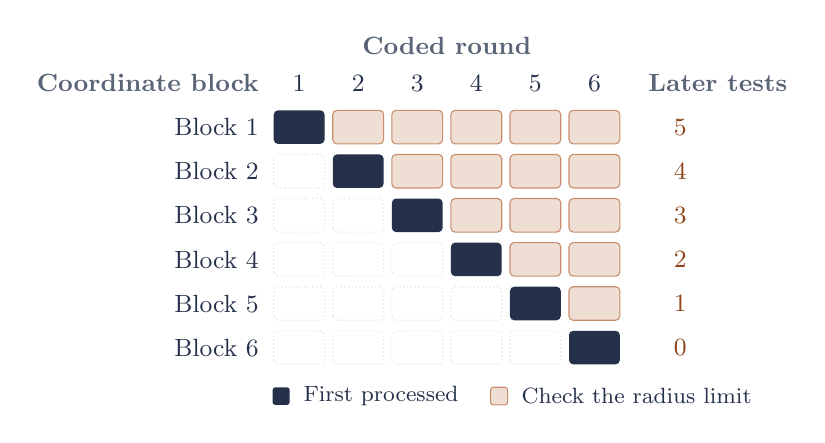
\begin{tikzpicture}[x=.75cm,y=.56cm,font=\small]
  \node[anchor=east,text=bkwmuted,font=\small\bfseries] at (.48,0) {Coordinate block};
  \node[text=bkwmuted,font=\small\bfseries] at (3.5,.85) {Coded round};
  \node[anchor=west,text=bkwmuted,font=\small\bfseries] at (6.75,0) {Later tests};
  \foreach \r in {1,...,6} {
    \node[text=bkwink] at (\r,0) {\r};
    \node[anchor=east,text=bkwink] at (.48,-\r) {Block \r};
    \pgfmathtruncatemacro{\later}{6-\r}
    \node[anchor=west,text=bkworange!85!black] at (7.18,-\r) {\later};
    \foreach \t in {1,...,6} {
      \ifnum\t<\r
        \draw[bkwline,rounded corners=1.5pt,densely dotted]
          (\t-.43,-\r-.38) rectangle (\t+.43,-\r+.38);
      \else
        \ifnum\t=\r
          \fill[bkwink,rounded corners=1.5pt]
            (\t-.43,-\r-.38) rectangle (\t+.43,-\r+.38);
        \else
          \filldraw[fill=bkworange!19,draw=bkworange!65,
                    rounded corners=1.5pt,line width=.4pt]
            (\t-.43,-\r-.38) rectangle (\t+.43,-\r+.38);
        \fi
      \fi
    }
  }
  \fill[bkwink,rounded corners=1pt] (.55,-7.30) rectangle (.84,-6.90);
  \node[anchor=west,text=bkwink,font=\footnotesize] at (.91,-7.1) {First processed};
  \filldraw[fill=bkworange!19,draw=bkworange!65,rounded corners=1pt]
    (4.24,-7.30) rectangle (4.53,-6.90);
  \node[anchor=west,text=bkwink,font=\footnotesize] at (4.60,-7.1) {Check the radius limit};
\end{tikzpicture}%
}
\caption{When each coordinate block is used, illustrated with six
coded rounds. Round~4, for example, groups the rows by block~4
and checks their differences on blocks~1--3. The first block
is checked in five later rounds. The last block is processed
only once.}
\label{fig:rounds-by-block}
\end{figure}

\paragraph{A separate radius for each block.}
We give each earlier block its own radius limit in each
later round. An early block faces more distance tests than a
late block. Its final radius is the starting radius times all
the later radius factors. Tighter limits later allow a larger
starting radius and therefore wider rounding bins and fewer
labels when the block first enters the list. They also make
qualifying pairs rarer. By setting the factors separately,
we can make this trade-off differently for each block.

Figure~\ref{fig:radius-factors} shows the change from the earlier
rule. A column represents one round. Earlier work applies the
same factor throughout that column; our schedule can contract
recent blocks while allowing some earlier blocks to grow.
Both choices serve the final radius requirements, but they
change the number of labels needed when each block is introduced.

\begin{figure}[!t]
\centering
\resizebox{.84\linewidth}{!}{%
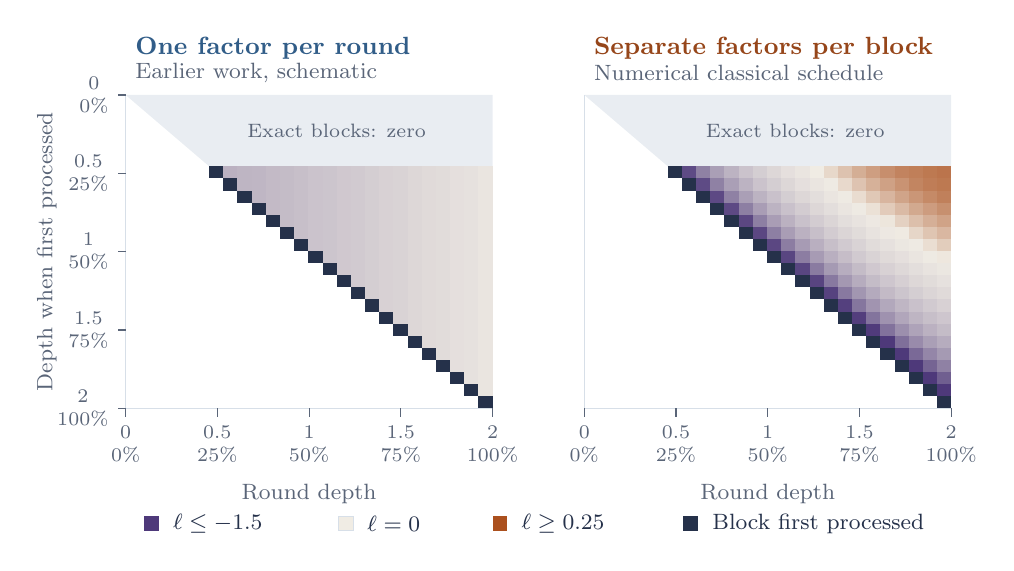
\begin{tikzpicture}[x=.233cm,y=.199cm,font=\footnotesize]
  \node[anchor=west,font=\small\bfseries,text=bkwblue] at (0,3.0) {One factor per round};
  \node[anchor=west,text=bkwmuted] at (0,1.4) {Earlier work, schematic};
  \node[anchor=west,font=\small\bfseries,text=bkworange!88!black] at (25,3.0) {Separate factors per block};
  \node[anchor=west,text=bkwmuted] at (25,1.4) {Numerical classical schedule};
  % The full schedule has depth 2. Exact-prefix blocks stay zero.
  \foreach \shift in {0,25} {
    \begin{scope}[shift={(\shift,0)}]
      \fill[bkwline!55!white] (0,0) -- (20,0) -- (20,-4.552106376) -- (4.552106376,-4.552106376) -- cycle;
      \node[text=bkwmuted,font=\scriptsize] at (11.5,-2.276053188) {Exact blocks: zero};
    \end{scope}
  }
  \begin{scope}[shift={(4.552106376,-4.552106376)},scale=0.772394681187]
  \foreach \j/\c in {0/bkwshrink!35!bkwneutral,1/bkwshrink!33!bkwneutral,2/bkwshrink!31!bkwneutral,3/bkwshrink!30!bkwneutral,4/bkwshrink!28!bkwneutral,5/bkwshrink!27!bkwneutral,6/bkwshrink!25!bkwneutral,7/bkwshrink!23!bkwneutral,8/bkwshrink!22!bkwneutral,9/bkwshrink!20!bkwneutral,10/bkwshrink!19!bkwneutral,11/bkwshrink!17!bkwneutral,12/bkwshrink!15!bkwneutral,13/bkwshrink!14!bkwneutral,14/bkwshrink!12!bkwneutral,15/bkwshrink!10!bkwneutral,16/bkwshrink!9!bkwneutral,17/bkwshrink!7!bkwneutral,18/bkwshrink!6!bkwneutral,19/bkwshrink!4!bkwneutral} {
    \fill[\c] (\j,0) rectangle (\j+1,-\j);
    \fill[bkwink] (\j,-\j) rectangle (\j+1,-\j-1);
  }
  \end{scope}
  \begin{scope}[shift={(29.552106376,-4.552106376)},scale=0.772394681187]
    % Values sampled from the classical solution, in equal intervals
    % of round depth. Diagonal entries indicate when each block is introduced.
    \foreach \j/\c in {0/bkwink,1/bkwshrink!90!bkwneutral,2/bkwshrink!60!bkwneutral,3/bkwshrink!43!bkwneutral,4/bkwshrink!32!bkwneutral,5/bkwshrink!23!bkwneutral,6/bkwshrink!17!bkwneutral,7/bkwshrink!12!bkwneutral,8/bkwshrink!7!bkwneutral,9/bkwshrink!4!bkwneutral,10/bkwshrink!0!bkwneutral,11/bkworange!13!bkwneutral,12/bkworange!27!bkwneutral,13/bkworange!40!bkwneutral,14/bkworange!50!bkwneutral,15/bkworange!60!bkwneutral,16/bkworange!67!bkwneutral,17/bkworange!70!bkwneutral,18/bkworange!74!bkwneutral,19/bkworange!77!bkwneutral} {\fill[\c] (\j,-0) rectangle (\j+1,-0-1);}
    \foreach \j/\c in {1/bkwink,2/bkwshrink!90!bkwneutral,3/bkwshrink!60!bkwneutral,4/bkwshrink!43!bkwneutral,5/bkwshrink!32!bkwneutral,6/bkwshrink!23!bkwneutral,7/bkwshrink!17!bkwneutral,8/bkwshrink!12!bkwneutral,9/bkwshrink!7!bkwneutral,10/bkwshrink!4!bkwneutral,11/bkwshrink!1!bkwneutral,12/bkworange!12!bkwneutral,13/bkworange!26!bkwneutral,14/bkworange!38!bkwneutral,15/bkworange!48!bkwneutral,16/bkworange!57!bkwneutral,17/bkworange!66!bkwneutral,18/bkworange!71!bkwneutral,19/bkworange!74!bkwneutral} {\fill[\c] (\j,-1) rectangle (\j+1,-1-1);}
    \foreach \j/\c in {2/bkwink,3/bkwshrink!91!bkwneutral,4/bkwshrink!60!bkwneutral,5/bkwshrink!43!bkwneutral,6/bkwshrink!32!bkwneutral,7/bkwshrink!24!bkwneutral,8/bkwshrink!17!bkwneutral,9/bkwshrink!12!bkwneutral,10/bkwshrink!8!bkwneutral,11/bkwshrink!4!bkwneutral,12/bkwshrink!1!bkwneutral,13/bkworange!10!bkwneutral,14/bkworange!23!bkwneutral,15/bkworange!35!bkwneutral,16/bkworange!46!bkwneutral,17/bkworange!55!bkwneutral,18/bkworange!63!bkwneutral,19/bkworange!69!bkwneutral} {\fill[\c] (\j,-2) rectangle (\j+1,-2-1);}
    \foreach \j/\c in {3/bkwink,4/bkwshrink!91!bkwneutral,5/bkwshrink!61!bkwneutral,6/bkwshrink!44!bkwneutral,7/bkwshrink!32!bkwneutral,8/bkwshrink!24!bkwneutral,9/bkwshrink!18!bkwneutral,10/bkwshrink!12!bkwneutral,11/bkwshrink!8!bkwneutral,12/bkwshrink!4!bkwneutral,13/bkwshrink!1!bkwneutral,14/bkworange!7!bkwneutral,15/bkworange!21!bkwneutral,16/bkworange!32!bkwneutral,17/bkworange!43!bkwneutral,18/bkworange!51!bkwneutral,19/bkworange!59!bkwneutral} {\fill[\c] (\j,-3) rectangle (\j+1,-3-1);}
    \foreach \j/\c in {4/bkwink,5/bkwshrink!92!bkwneutral,6/bkwshrink!61!bkwneutral,7/bkwshrink!44!bkwneutral,8/bkwshrink!33!bkwneutral,9/bkwshrink!24!bkwneutral,10/bkwshrink!18!bkwneutral,11/bkwshrink!13!bkwneutral,12/bkwshrink!8!bkwneutral,13/bkwshrink!5!bkwneutral,14/bkwshrink!2!bkwneutral,15/bkworange!4!bkwneutral,16/bkworange!17!bkwneutral,17/bkworange!29!bkwneutral,18/bkworange!39!bkwneutral,19/bkworange!47!bkwneutral} {\fill[\c] (\j,-4) rectangle (\j+1,-4-1);}
    \foreach \j/\c in {5/bkwink,6/bkwshrink!92!bkwneutral,7/bkwshrink!61!bkwneutral,8/bkwshrink!44!bkwneutral,9/bkwshrink!33!bkwneutral,10/bkwshrink!25!bkwneutral,11/bkwshrink!18!bkwneutral,12/bkwshrink!13!bkwneutral,13/bkwshrink!9!bkwneutral,14/bkwshrink!5!bkwneutral,15/bkwshrink!2!bkwneutral,16/bkworange!1!bkwneutral,17/bkworange!14!bkwneutral,18/bkworange!25!bkwneutral,19/bkworange!34!bkwneutral} {\fill[\c] (\j,-5) rectangle (\j+1,-5-1);}
    \foreach \j/\c in {6/bkwink,7/bkwshrink!92!bkwneutral,8/bkwshrink!62!bkwneutral,9/bkwshrink!45!bkwneutral,10/bkwshrink!34!bkwneutral,11/bkwshrink!25!bkwneutral,12/bkwshrink!19!bkwneutral,13/bkwshrink!14!bkwneutral,14/bkwshrink!9!bkwneutral,15/bkwshrink!6!bkwneutral,16/bkwshrink!3!bkwneutral,17/bkwshrink!1!bkwneutral,18/bkworange!9!bkwneutral,19/bkworange!20!bkwneutral} {\fill[\c] (\j,-6) rectangle (\j+1,-6-1);}
    \foreach \j/\c in {7/bkwink,8/bkwshrink!93!bkwneutral,9/bkwshrink!62!bkwneutral,10/bkwshrink!45!bkwneutral,11/bkwshrink!34!bkwneutral,12/bkwshrink!26!bkwneutral,13/bkwshrink!19!bkwneutral,14/bkwshrink!14!bkwneutral,15/bkwshrink!10!bkwneutral,16/bkwshrink!7!bkwneutral,17/bkwshrink!4!bkwneutral,18/bkwshrink!1!bkwneutral,19/bkworange!3!bkwneutral} {\fill[\c] (\j,-7) rectangle (\j+1,-7-1);}
    \foreach \j/\c in {8/bkwink,9/bkwshrink!93!bkwneutral,10/bkwshrink!63!bkwneutral,11/bkwshrink!46!bkwneutral,12/bkwshrink!35!bkwneutral,13/bkwshrink!27!bkwneutral,14/bkwshrink!20!bkwneutral,15/bkwshrink!15!bkwneutral,16/bkwshrink!11!bkwneutral,17/bkwshrink!8!bkwneutral,18/bkwshrink!5!bkwneutral,19/bkwshrink!3!bkwneutral} {\fill[\c] (\j,-8) rectangle (\j+1,-8-1);}
    \foreach \j/\c in {9/bkwink,10/bkwshrink!94!bkwneutral,11/bkwshrink!64!bkwneutral,12/bkwshrink!47!bkwneutral,13/bkwshrink!36!bkwneutral,14/bkwshrink!27!bkwneutral,15/bkwshrink!21!bkwneutral,16/bkwshrink!16!bkwneutral,17/bkwshrink!12!bkwneutral,18/bkwshrink!9!bkwneutral,19/bkwshrink!6!bkwneutral} {\fill[\c] (\j,-9) rectangle (\j+1,-9-1);}
    \foreach \j/\c in {10/bkwink,11/bkwshrink!95!bkwneutral,12/bkwshrink!64!bkwneutral,13/bkwshrink!48!bkwneutral,14/bkwshrink!37!bkwneutral,15/bkwshrink!28!bkwneutral,16/bkwshrink!22!bkwneutral,17/bkwshrink!17!bkwneutral,18/bkwshrink!13!bkwneutral,19/bkwshrink!10!bkwneutral} {\fill[\c] (\j,-10) rectangle (\j+1,-10-1);}
    \foreach \j/\c in {11/bkwink,12/bkwshrink!96!bkwneutral,13/bkwshrink!66!bkwneutral,14/bkwshrink!49!bkwneutral,15/bkwshrink!38!bkwneutral,16/bkwshrink!30!bkwneutral,17/bkwshrink!24!bkwneutral,18/bkwshrink!19!bkwneutral,19/bkwshrink!15!bkwneutral} {\fill[\c] (\j,-11) rectangle (\j+1,-11-1);}
    \foreach \j/\c in {12/bkwink,13/bkwshrink!97!bkwneutral,14/bkwshrink!67!bkwneutral,15/bkwshrink!50!bkwneutral,16/bkwshrink!39!bkwneutral,17/bkwshrink!31!bkwneutral,18/bkwshrink!25!bkwneutral,19/bkwshrink!21!bkwneutral} {\fill[\c] (\j,-12) rectangle (\j+1,-12-1);}
    \foreach \j/\c in {13/bkwink,14/bkwshrink!99!bkwneutral,15/bkwshrink!68!bkwneutral,16/bkwshrink!52!bkwneutral,17/bkwshrink!41!bkwneutral,18/bkwshrink!33!bkwneutral,19/bkwshrink!27!bkwneutral} {\fill[\c] (\j,-13) rectangle (\j+1,-13-1);}
    \foreach \j/\c in {14/bkwink,15/bkwshrink!100!bkwneutral,16/bkwshrink!70!bkwneutral,17/bkwshrink!54!bkwneutral,18/bkwshrink!43!bkwneutral,19/bkwshrink!36!bkwneutral} {\fill[\c] (\j,-14) rectangle (\j+1,-14-1);}
    \foreach \j/\c in {15/bkwink,16/bkwshrink!100!bkwneutral,17/bkwshrink!73!bkwneutral,18/bkwshrink!57!bkwneutral,19/bkwshrink!46!bkwneutral} {\fill[\c] (\j,-15) rectangle (\j+1,-15-1);}
    \foreach \j/\c in {16/bkwink,17/bkwshrink!100!bkwneutral,18/bkwshrink!76!bkwneutral,19/bkwshrink!60!bkwneutral} {\fill[\c] (\j,-16) rectangle (\j+1,-16-1);}
    \foreach \j/\c in {17/bkwink,18/bkwshrink!100!bkwneutral,19/bkwshrink!79!bkwneutral} {\fill[\c] (\j,-17) rectangle (\j+1,-17-1);}
    \foreach \j/\c in {18/bkwink,19/bkwshrink!100!bkwneutral} {\fill[\c] (\j,-18) rectangle (\j+1,-18-1);}
    \foreach \j/\c in {19/bkwink} {\fill[\c] (\j,-19) rectangle (\j+1,-19-1);}
  \end{scope}
  \foreach \shift in {0,25} {
    \begin{scope}[shift={(\shift,0)}]
      \draw[bkwline] (0,0) -- (0,-20) -- (20,-20);
      \foreach \xx/\lbl/\pct in {0/0/0,5/0.5/25,10/1/50,15/1.5/75,20/2/100} {
        \draw[bkwmuted] (\xx,-20) -- (\xx,-20.52);
        \node[below,text=bkwmuted,font=\scriptsize] at (\xx,-20.52) {\shortstack{\lbl\\\pct\%}};
      }
      \node[below,text=bkwmuted] at (10,-24.2) {Round depth};
    \end{scope}
  }
  \foreach \xx/\lbl/\pct in {0/0/0,5/0.5/25,10/1/50,15/1.5/75,20/2/100} {
    \draw[bkwmuted] (0,-\xx) -- (-.4,-\xx);
    \node[left,text=bkwmuted,font=\scriptsize] at (-.4,-\xx) {\shortstack{\lbl\\\pct\%}};
  }
  \node[rotate=90,text=bkwmuted] at (-4.3,-10) {Depth when first processed};
  \fill[bkwshrink] (1.0,-27.8) rectangle (1.8,-26.9);
  \node[anchor=west,text=bkwink] at (2.05,-27.35) {$\ell\le -1.5$};
  \filldraw[fill=bkwneutral,draw=bkwline] (11.6,-27.8) rectangle (12.4,-26.9);
  \node[anchor=west,text=bkwink] at (12.65,-27.35) {$\ell=0$};
  \fill[bkworange] (20,-27.8) rectangle (20.8,-26.9);
  \node[anchor=west,text=bkwink] at (21.05,-27.35) {$\ell\ge0.25$};
  \fill[bkwink] (30.4,-27.8) rectangle (31.2,-26.9);
  \node[anchor=west,text=bkwink] at (31.45,-27.35) {Block first processed};
\end{tikzpicture}%
}
\caption{Radius factors in earlier work and in the classical algorithm of
Theorem~\ref{thm:classical}. Color gives $\ell=\log_2$ of the radius factor.
Both axes cover the full schedule: depth $t$ means $t\log_2 n$ rounds,
so $0$--$2$ corresponds to $0\%$--$100\%$ of all rounds; each tick shows
both scales. Gray regions have no coded-radius test: exact blocks remain
zero. The coded phase begins at depth $0.4552\ldots$.
The left schematic has one factor per column, as in \cite{M19};
the right uses the solution of \eqref{eq:shared-forward} and
\eqref{eq:shared-clock}. Recently processed coded blocks are often
contracted more strongly, while some early coded blocks grow late.}
\label{fig:radius-factors}
\end{figure}

\paragraph{Choosing the block sizes.}
The block sizes and radius limits must be chosen together.
A round's search cost depends on every earlier block; a block's
starting radius depends on its later tests. We first calculate
how many coordinates enter each round, working from the first
round onward. We then calculate the round lengths backward
from the last round. Integral equations express these two
calculations. Finally, we keep enough rows at each step to
supply the later rounds. The same calculation works with
each of the three pair searches.

The quantum variants use their own radius choices, block sizes,
and split between exact and coded rounds. All three use
$(2+o(1))\log_2 n$ rounds. To leading order, the exact prefixes
use about $0.4552$, $0.2686$, and $0.1762$ times $\log_2 n$ rounds
for classical search, Grover search, and the walk, respectively. Thus the coded phase occupies $77.24\%$, $86.57\%$,
and $91.19\%$ of the rounds. Figure~\ref{fig:block-size-profile}
compares the resulting block sizes on the same round scale.
The quantum schedules have larger first coded blocks and smaller
last blocks. Earlier work already permits unequal blocks and different quantum
parameters~\cite[Sections~III--V]{M19}; here the optimization also
chooses a separate radius for every earlier block.

\begin{figure}[!t]
\centering
\resizebox{.84\linewidth}{!}{%
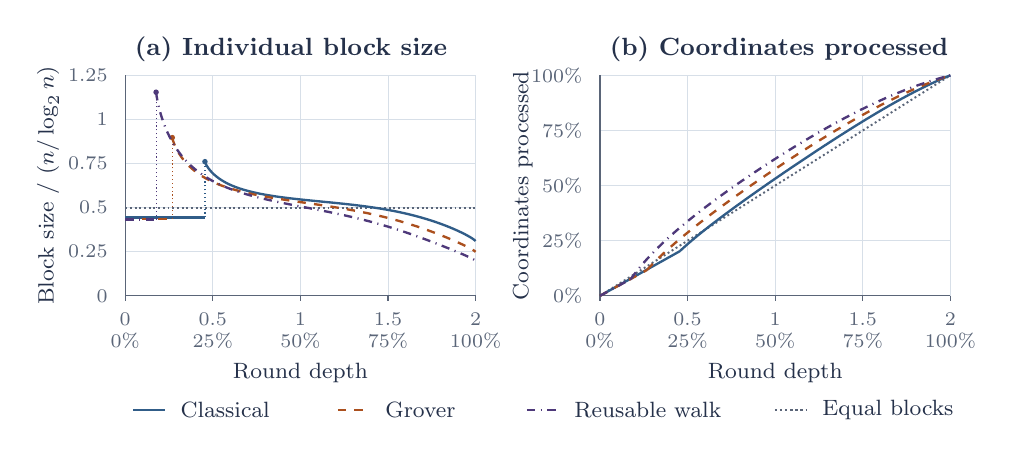
\begin{tikzpicture}[x=1cm,y=1cm,font=\footnotesize]
\begin{scope}[shift={(0,0)}]
\node[anchor=west,font=\small\bfseries,text=bkwink] at (0,3.13) {(a) Individual block size};
\draw[bkwline,line width=.3pt] (0,0.000000) -- (4.45,0.000000);
\node[anchor=east,text=bkwmuted,font=\scriptsize] at (-.10,0.000000) {0};
\draw[bkwline,line width=.3pt] (0,0.560000) -- (4.45,0.560000);
\node[anchor=east,text=bkwmuted,font=\scriptsize] at (-.10,0.560000) {0.25};
\draw[bkwline,line width=.3pt] (0,1.120000) -- (4.45,1.120000);
\node[anchor=east,text=bkwmuted,font=\scriptsize] at (-.10,1.120000) {0.5};
\draw[bkwline,line width=.3pt] (0,1.680000) -- (4.45,1.680000);
\node[anchor=east,text=bkwmuted,font=\scriptsize] at (-.10,1.680000) {0.75};
\draw[bkwline,line width=.3pt] (0,2.240000) -- (4.45,2.240000);
\node[anchor=east,text=bkwmuted,font=\scriptsize] at (-.10,2.240000) {1};
\draw[bkwline,line width=.3pt] (0,2.800000) -- (4.45,2.800000);
\node[anchor=east,text=bkwmuted,font=\scriptsize] at (-.10,2.800000) {1.25};
\draw[bkwline,line width=.3pt] (1.112500,0) -- (1.112500,2.8);
\draw[bkwline,line width=.3pt] (2.225000,0) -- (2.225000,2.8);
\draw[bkwline,line width=.3pt] (3.337500,0) -- (3.337500,2.8);
\draw[bkwline,line width=.3pt] (4.450000,0) -- (4.450000,2.8);
\draw[bkwmuted,line width=.4pt] (0,2.8) -- (0,0) -- (4.45,0);
\draw[bkwmuted,line width=.4pt] (0.000000,0) -- (0.000000,-.06);
\node[below,text=bkwmuted,font=\scriptsize] at (0.000000,-.09) {\shortstack{0\\0\%}};
\draw[bkwmuted,line width=.4pt] (1.112500,0) -- (1.112500,-.06);
\node[below,text=bkwmuted,font=\scriptsize] at (1.112500,-.09) {\shortstack{0.5\\25\%}};
\draw[bkwmuted,line width=.4pt] (2.225000,0) -- (2.225000,-.06);
\node[below,text=bkwmuted,font=\scriptsize] at (2.225000,-.09) {\shortstack{1\\50\%}};
\draw[bkwmuted,line width=.4pt] (3.337500,0) -- (3.337500,-.06);
\node[below,text=bkwmuted,font=\scriptsize] at (3.337500,-.09) {\shortstack{1.5\\75\%}};
\draw[bkwmuted,line width=.4pt] (4.450000,0) -- (4.450000,-.06);
\node[below,text=bkwmuted,font=\scriptsize] at (4.450000,-.09) {\shortstack{2\\100\%}};
\node[text=bkwink] at (2.225,-.98) {Round depth};
\node[rotate=90,text=bkwink] at (-.98,1.4) {Block size / $(n/\log_2 n)$};
\draw[bkwmuted,densely dotted,line width=.7pt] (0,1.120000) -- (4.45,1.120000);
\draw[bkwblue,solid,line width=.85pt,line join=round] plot coordinates {(0.000000,0.994842) (1.012844,0.994842)};
\draw[bkwblue,densely dotted,line width=.4pt] (1.012844,0.994842) -- (1.012844,1.703488);
\fill[bkwblue] (1.012844,1.703488) circle (1pt);
\draw[bkwblue,solid,line width=.85pt,line join=round] plot coordinates {
(1.012844,1.703488) (1.019718,1.684258) (1.026592,1.669663) (1.033467,1.656852) (1.040341,1.645209)
(1.047215,1.634435) (1.054090,1.624357) (1.060964,1.614857) (1.067838,1.605850) (1.074712,1.597274)
(1.081587,1.589079) (1.088461,1.581227) (1.095335,1.573684) (1.102210,1.566424) (1.109084,1.559424)
(1.115958,1.552663) (1.122833,1.546125) (1.129707,1.539794) (1.136581,1.533658) (1.143456,1.527705)
(1.150330,1.521923) (1.157204,1.516304) (1.164079,1.510838) (1.170953,1.505519) (1.177827,1.500338)
(1.184701,1.495289) (1.191576,1.490366) (1.198450,1.485564) (1.205324,1.480877) (1.212199,1.476300)
(1.219073,1.471830) (1.225947,1.467461) (1.232822,1.463191) (1.239696,1.459014) (1.246570,1.454929)
(1.253445,1.450931) (1.260319,1.447018) (1.267193,1.443187) (1.274068,1.439435) (1.280942,1.435760)
(1.287816,1.432159) (1.294690,1.428629) (1.301565,1.425170) (1.308439,1.421778) (1.315313,1.418452)
(1.322188,1.415190) (1.329062,1.411991) (1.335936,1.408851) (1.342811,1.405771) (1.349685,1.402748)
(1.356559,1.399781) (1.363434,1.396868) (1.370308,1.394009) (1.377182,1.391201) (1.384057,1.388444)
(1.390931,1.385737) (1.397805,1.383078) (1.404679,1.380466) (1.411554,1.377901) (1.418428,1.375381)
(1.425302,1.372905) (1.432177,1.370473) (1.439051,1.368084) (1.445925,1.365737) (1.452800,1.363431)
(1.459674,1.361165) (1.466548,1.358934) (1.473423,1.356737) (1.480297,1.354573) (1.487171,1.352440)
(1.494046,1.350339) (1.500920,1.348268) (1.507794,1.346227) (1.514668,1.344215) (1.521543,1.342232)
(1.528417,1.340277) (1.535291,1.338349) (1.542166,1.336448) (1.549040,1.334573) (1.555914,1.332724)
(1.562789,1.330900) (1.569663,1.329100) (1.576537,1.327325) (1.583412,1.325574) (1.590286,1.323846)
(1.597160,1.322140) (1.604035,1.320457) (1.610909,1.318795) (1.617783,1.317155) (1.624657,1.315536)
(1.631532,1.313938) (1.638406,1.312359) (1.645280,1.310801) (1.652155,1.309262) (1.659029,1.307742)
(1.665903,1.306241) (1.672778,1.304758) (1.679652,1.303293) (1.686526,1.301845) (1.693401,1.300415)
(1.700275,1.299002) (1.707149,1.297606) (1.714024,1.296226) (1.720898,1.294862) (1.727772,1.293514)
(1.734646,1.292181) (1.741521,1.290863) (1.748395,1.289561) (1.755269,1.288273) (1.762144,1.286999)
(1.769018,1.285740) (1.775892,1.284494) (1.782767,1.283262) (1.789641,1.282044) (1.796515,1.280838)
(1.803390,1.279646) (1.810264,1.278466) (1.817138,1.277298) (1.824013,1.276143) (1.830887,1.274999)
(1.837761,1.273868) (1.844636,1.272748) (1.851510,1.271639) (1.858384,1.270541) (1.865258,1.269454)
(1.872133,1.268378) (1.879007,1.267313) (1.885881,1.266258) (1.892756,1.265213) (1.899630,1.264178)
(1.906504,1.263152) (1.913379,1.262137) (1.920253,1.261130) (1.927127,1.260133) (1.934002,1.259146)
(1.940876,1.258166) (1.947750,1.257196) (1.954625,1.256234) (1.961499,1.255281) (1.968373,1.254336)
(1.975247,1.253399) (1.982122,1.252470) (1.988996,1.251549) (1.995870,1.250635) (2.002745,1.249729)
(2.009619,1.248830) (2.016493,1.247938) (2.023368,1.247054) (2.030242,1.246176) (2.037116,1.245305)
(2.043991,1.244441) (2.050865,1.243583) (2.057739,1.242732) (2.064614,1.241887) (2.071488,1.241048)
(2.078362,1.240215) (2.085236,1.239387) (2.092111,1.238566) (2.098985,1.237750) (2.105859,1.236939)
(2.112734,1.236134) (2.119608,1.235334) (2.126482,1.234540) (2.133357,1.233750) (2.140231,1.232965)
(2.147105,1.232185) (2.153980,1.231409) (2.160854,1.230638) (2.167728,1.229872) (2.174603,1.229110)
(2.181477,1.228352) (2.188351,1.227598) (2.195225,1.226848) (2.202100,1.226102) (2.208974,1.225360)
(2.215848,1.224621) (2.222723,1.223886) (2.229597,1.223154) (2.236471,1.222426) (2.243346,1.221701)
(2.250220,1.220979) (2.257094,1.220261) (2.263969,1.219545) (2.270843,1.218832) (2.277717,1.218122)
(2.284592,1.217414) (2.291466,1.216710) (2.298340,1.216007) (2.305214,1.215307) (2.312089,1.214609)
(2.318963,1.213914) (2.325837,1.213221) (2.332712,1.212529) (2.339586,1.211840) (2.346460,1.211152)
(2.353335,1.210466) (2.360209,1.209782) (2.367083,1.209100) (2.373958,1.208418) (2.380832,1.207739)
(2.387706,1.207060) (2.394581,1.206383) (2.401455,1.205707) (2.408329,1.205032) (2.415203,1.204358)
(2.422078,1.203685) (2.428952,1.203013) (2.435826,1.202341) (2.442701,1.201670) (2.449575,1.201000)
(2.456449,1.200330) (2.463324,1.199660) (2.470198,1.198991) (2.477072,1.198322) (2.483947,1.197653)
(2.490821,1.196984) (2.497695,1.196315) (2.504570,1.195646) (2.511444,1.194977) (2.518318,1.194307)
(2.525192,1.193638) (2.532067,1.192968) (2.538941,1.192297) (2.545815,1.191626) (2.552690,1.190954)
(2.559564,1.190281) (2.566438,1.189608) (2.573313,1.188933) (2.580187,1.188258) (2.587061,1.187582)
(2.593936,1.186904) (2.600810,1.186226) (2.607684,1.185546) (2.614559,1.184865) (2.621433,1.184182)
(2.628307,1.183498) (2.635181,1.182812) (2.642056,1.182125) (2.648930,1.181436) (2.655804,1.180745)
(2.662679,1.180052) (2.669553,1.179357) (2.676427,1.178660) (2.683302,1.177962) (2.690176,1.177261)
(2.697050,1.176557) (2.703925,1.175852) (2.710799,1.175144) (2.717673,1.174433) (2.724548,1.173720)
(2.731422,1.173005) (2.738296,1.172286) (2.745170,1.171565) (2.752045,1.170841) (2.758919,1.170114)
(2.765793,1.169384) (2.772668,1.168651) (2.779542,1.167915) (2.786416,1.167176) (2.793291,1.166434)
(2.800165,1.165688) (2.807039,1.164938) (2.813914,1.164185) (2.820788,1.163429) (2.827662,1.162669)
(2.834537,1.161905) (2.841411,1.161137) (2.848285,1.160366) (2.855159,1.159590) (2.862034,1.158811)
(2.868908,1.158027) (2.875782,1.157239) (2.882657,1.156447) (2.889531,1.155651) (2.896405,1.154850)
(2.903280,1.154045) (2.910154,1.153235) (2.917028,1.152421) (2.923903,1.151602) (2.930777,1.150778)
(2.937651,1.149949) (2.944526,1.149116) (2.951400,1.148277) (2.958274,1.147434) (2.965148,1.146585)
(2.972023,1.145731) (2.978897,1.144872) (2.985771,1.144007) (2.992646,1.143137) (2.999520,1.142262)
(3.006394,1.141381) (3.013269,1.140494) (3.020143,1.139602) (3.027017,1.138703) (3.033892,1.137799)
(3.040766,1.136889) (3.047640,1.135973) (3.054515,1.135051) (3.061389,1.134123) (3.068263,1.133188)
(3.075137,1.132247) (3.082012,1.131300) (3.088886,1.130346) (3.095760,1.129386) (3.102635,1.128419)
(3.109509,1.127445) (3.116383,1.126465) (3.123258,1.125477) (3.130132,1.124483) (3.137006,1.123482)
(3.143881,1.122474) (3.150755,1.121459) (3.157629,1.120436) (3.164504,1.119406) (3.171378,1.118369)
(3.178252,1.117324) (3.185126,1.116272) (3.192001,1.115212) (3.198875,1.114144) (3.205749,1.113069)
(3.212624,1.111986) (3.219498,1.110895) (3.226372,1.109796) (3.233247,1.108689) (3.240121,1.107574)
(3.246995,1.106451) (3.253870,1.105319) (3.260744,1.104179) (3.267618,1.103031) (3.274493,1.101874)
(3.281367,1.100709) (3.288241,1.099534) (3.295115,1.098352) (3.301990,1.097160) (3.308864,1.095959)
(3.315738,1.094750) (3.322613,1.093531) (3.329487,1.092304) (3.336361,1.091067) (3.343236,1.089821)
(3.350110,1.088565) (3.356984,1.087300) (3.363859,1.086026) (3.370733,1.084742) (3.377607,1.083448)
(3.384482,1.082145) (3.391356,1.080832) (3.398230,1.079509) (3.405104,1.078176) (3.411979,1.076833)
(3.418853,1.075480) (3.425727,1.074117) (3.432602,1.072743) (3.439476,1.071360) (3.446350,1.069965)
(3.453225,1.068561) (3.460099,1.067145) (3.466973,1.065719) (3.473848,1.064283) (3.480722,1.062835)
(3.487596,1.061377) (3.494471,1.059908) (3.501345,1.058428) (3.508219,1.056937) (3.515093,1.055434)
(3.521968,1.053920) (3.528842,1.052395) (3.535716,1.050859) (3.542591,1.049311) (3.549465,1.047752)
(3.556339,1.046181) (3.563214,1.044598) (3.570088,1.043004) (3.576962,1.041397) (3.583837,1.039779)
(3.590711,1.038149) (3.597585,1.036507) (3.604460,1.034852) (3.611334,1.033185) (3.618208,1.031506)
(3.625082,1.029815) (3.631957,1.028111) (3.638831,1.026395) (3.645705,1.024666) (3.652580,1.022924)
(3.659454,1.021169) (3.666328,1.019402) (3.673203,1.017622) (3.680077,1.015828) (3.686951,1.014022)
(3.693826,1.012202) (3.700700,1.010370) (3.707574,1.008524) (3.714449,1.006665) (3.721323,1.004792)
(3.728197,1.002906) (3.735071,1.001006) (3.741946,0.999093) (3.748820,0.997166) (3.755694,0.995226)
(3.762569,0.993272) (3.769443,0.991303) (3.776317,0.989321) (3.783192,0.987325) (3.790066,0.985315)
(3.796940,0.983290) (3.803815,0.981252) (3.810689,0.979199) (3.817563,0.977131) (3.824438,0.975050)
(3.831312,0.972953) (3.838186,0.970842) (3.845060,0.968717) (3.851935,0.966576) (3.858809,0.964421)
(3.865683,0.962251) (3.872558,0.960066) (3.879432,0.957866) (3.886306,0.955650) (3.893181,0.953420)
(3.900055,0.951174) (3.906929,0.948912) (3.913804,0.946635) (3.920678,0.944343) (3.927552,0.942034)
(3.934427,0.939710) (3.941301,0.937370) (3.948175,0.935014) (3.955049,0.932642) (3.961924,0.930254)
(3.968798,0.927849) (3.975672,0.925428) (3.982547,0.922991) (3.989421,0.920536) (3.996295,0.918065)
(4.003170,0.915578) (4.010044,0.913073) (4.016918,0.910551) (4.023793,0.908011) (4.030667,0.905455)
(4.037541,0.902881) (4.044416,0.900289) (4.051290,0.897679) (4.058164,0.895051) (4.065038,0.892405)
(4.071913,0.889741) (4.078787,0.887058) (4.085661,0.884357) (4.092536,0.881636) (4.099410,0.878897)
(4.106284,0.876138) (4.113159,0.873360) (4.120033,0.870562) (4.126907,0.867744) (4.133782,0.864906)
(4.140656,0.862047) (4.147530,0.859168) (4.154405,0.856267) (4.161279,0.853345) (4.168153,0.850401)
(4.175027,0.847436) (4.181902,0.844447) (4.188776,0.841436) (4.195650,0.838402) (4.202525,0.835344)
(4.209399,0.832261) (4.216273,0.829154) (4.223148,0.826022) (4.230022,0.822864) (4.236896,0.819680)
(4.243771,0.816468) (4.250645,0.813229) (4.257519,0.809961) (4.264394,0.806663) (4.271268,0.803335)
(4.278142,0.799975) (4.285016,0.796583) (4.291891,0.793158) (4.298765,0.789697) (4.305639,0.786199)
(4.312514,0.782664) (4.319388,0.779088) (4.326262,0.775471) (4.333137,0.771809) (4.340011,0.768100)
(4.346885,0.764341) (4.353760,0.760529) (4.360634,0.756659) (4.367508,0.752728) (4.374383,0.748730)
(4.381257,0.744658) (4.388131,0.740505) (4.395005,0.736260) (4.401880,0.731911) (4.408754,0.727442)
(4.415628,0.722831) (4.422503,0.718047) (4.429377,0.713041) (4.436251,0.707729) (4.443126,0.701933)
(4.450000,0.694783)
};
\draw[bkworange,dashed,line width=.85pt,line join=round] plot coordinates {(0.000000,0.978514) (0.597646,0.978514)};
\draw[bkworange,densely dotted,line width=.4pt] (0.597646,0.978514) -- (0.597646,2.009169);
\fill[bkworange] (0.597646,2.009169) circle (1pt);
\draw[bkworange,dashed,line width=.85pt,line join=round] plot coordinates {
(0.597646,2.009169) (0.605351,1.977852) (0.613056,1.953986) (0.620761,1.933019) (0.628465,1.913961)
(0.636170,1.896332) (0.643875,1.879846) (0.651579,1.864313) (0.659284,1.849596) (0.666989,1.835592)
(0.674693,1.822219) (0.682398,1.809412) (0.690103,1.797118) (0.697808,1.785292) (0.705512,1.773897)
(0.713217,1.762898) (0.720922,1.752268) (0.728626,1.741982) (0.736331,1.732017) (0.744036,1.722353)
(0.751741,1.712974) (0.759445,1.703863) (0.767150,1.695005) (0.774855,1.686388) (0.782559,1.677999)
(0.790264,1.669827) (0.797969,1.661862) (0.805673,1.654095) (0.813378,1.646517) (0.821083,1.639120)
(0.828788,1.631896) (0.836492,1.624839) (0.844197,1.617941) (0.851902,1.611198) (0.859606,1.604602)
(0.867311,1.598149) (0.875016,1.591833) (0.882721,1.585650) (0.890425,1.579595) (0.898130,1.573664)
(0.905835,1.567852) (0.913539,1.562157) (0.921244,1.556573) (0.928949,1.551099) (0.936654,1.545730)
(0.944358,1.540463) (0.952063,1.535296) (0.959768,1.530226) (0.967472,1.525249) (0.975177,1.520363)
(0.982882,1.515566) (0.990586,1.510856) (0.998291,1.506229) (1.005996,1.501685) (1.013701,1.497220)
(1.021405,1.492834) (1.029110,1.488523) (1.036815,1.484287) (1.044519,1.480122) (1.052224,1.476029)
(1.059929,1.472005) (1.067634,1.468048) (1.075338,1.464157) (1.083043,1.460331) (1.090748,1.456569)
(1.098452,1.452868) (1.106157,1.449228) (1.113862,1.445647) (1.121566,1.442125) (1.129271,1.438660)
(1.136976,1.435251) (1.144681,1.431897) (1.152385,1.428597) (1.160090,1.425351) (1.167795,1.422157)
(1.175499,1.419014) (1.183204,1.415922) (1.190909,1.412880) (1.198614,1.409887) (1.206318,1.406943)
(1.214023,1.404046) (1.221728,1.401188) (1.229432,1.398369) (1.237137,1.395586) (1.244842,1.392839)
(1.252547,1.390127) (1.260251,1.387450) (1.267956,1.384807) (1.275661,1.382197) (1.283365,1.379620)
(1.291070,1.377074) (1.298775,1.374560) (1.306479,1.372076) (1.314184,1.369623) (1.321889,1.367199)
(1.329594,1.364803) (1.337298,1.362436) (1.345003,1.360097) (1.352708,1.357785) (1.360412,1.355500)
(1.368117,1.353240) (1.375822,1.351007) (1.383527,1.348798) (1.391231,1.346615) (1.398936,1.344455)
(1.406641,1.342320) (1.414345,1.340207) (1.422050,1.338118) (1.429755,1.336051) (1.437459,1.334006)
(1.445164,1.331982) (1.452869,1.329980) (1.460574,1.327999) (1.468278,1.326038) (1.475983,1.324097)
(1.483688,1.322176) (1.491392,1.320274) (1.499097,1.318391) (1.506802,1.316527) (1.514507,1.314681)
(1.522211,1.312853) (1.529916,1.311042) (1.537621,1.309249) (1.545325,1.307473) (1.553030,1.305713)
(1.560735,1.303970) (1.568440,1.302243) (1.576144,1.300531) (1.583849,1.298835) (1.591554,1.297154)
(1.599258,1.295488) (1.606963,1.293836) (1.614668,1.292199) (1.622372,1.290576) (1.630077,1.288967)
(1.637782,1.287371) (1.645487,1.285788) (1.653191,1.284219) (1.660896,1.282662) (1.668601,1.281118)
(1.676305,1.279586) (1.684010,1.278066) (1.691715,1.276558) (1.699420,1.275061) (1.707124,1.273576)
(1.714829,1.272102) (1.722534,1.270639) (1.730238,1.269186) (1.737943,1.267745) (1.745648,1.266313)
(1.753352,1.264891) (1.761057,1.263480) (1.768762,1.262078) (1.776467,1.260685) (1.784171,1.259302)
(1.791876,1.257928) (1.799581,1.256563) (1.807285,1.255206) (1.814990,1.253858) (1.822695,1.252518)
(1.830400,1.251187) (1.838104,1.249863) (1.845809,1.248547) (1.853514,1.247239) (1.861218,1.245939)
(1.868923,1.244645) (1.876628,1.243359) (1.884333,1.242080) (1.892037,1.240807) (1.899742,1.239541)
(1.907447,1.238281) (1.915151,1.237028) (1.922856,1.235781) (1.930561,1.234540) (1.938265,1.233305)
(1.945970,1.232075) (1.953675,1.230851) (1.961380,1.229632) (1.969084,1.228419) (1.976789,1.227211)
(1.984494,1.226007) (1.992198,1.224809) (1.999903,1.223615) (2.007608,1.222425) (2.015313,1.221240)
(2.023017,1.220059) (2.030722,1.218882) (2.038427,1.217709) (2.046131,1.216540) (2.053836,1.215375)
(2.061541,1.214213) (2.069245,1.213055) (2.076950,1.211900) (2.084655,1.210748) (2.092360,1.209599)
(2.100064,1.208453) (2.107769,1.207310) (2.115474,1.206169) (2.123178,1.205031) (2.130883,1.203896)
(2.138588,1.202762) (2.146293,1.201631) (2.153997,1.200502) (2.161702,1.199375) (2.169407,1.198250)
(2.177111,1.197126) (2.184816,1.196004) (2.192521,1.194883) (2.200225,1.193764) (2.207930,1.192645)
(2.215635,1.191528) (2.223340,1.190412) (2.231044,1.189297) (2.238749,1.188183) (2.246454,1.187069)
(2.254158,1.185956) (2.261863,1.184843) (2.269568,1.183730) (2.277273,1.182618) (2.284977,1.181506)
(2.292682,1.180394) (2.300387,1.179281) (2.308091,1.178169) (2.315796,1.177056) (2.323501,1.175943)
(2.331206,1.174829) (2.338910,1.173714) (2.346615,1.172599) (2.354320,1.171483) (2.362024,1.170365)
(2.369729,1.169247) (2.377434,1.168128) (2.385138,1.167007) (2.392843,1.165885) (2.400548,1.164762)
(2.408253,1.163637) (2.415957,1.162510) (2.423662,1.161381) (2.431367,1.160251) (2.439071,1.159118)
(2.446776,1.157984) (2.454481,1.156847) (2.462186,1.155708) (2.469890,1.154567) (2.477595,1.153423)
(2.485300,1.152276) (2.493004,1.151127) (2.500709,1.149975) (2.508414,1.148820) (2.516118,1.147663)
(2.523823,1.146502) (2.531528,1.145338) (2.539233,1.144171) (2.546937,1.143000) (2.554642,1.141826)
(2.562347,1.140648) (2.570051,1.139467) (2.577756,1.138282) (2.585461,1.137093) (2.593166,1.135901)
(2.600870,1.134704) (2.608575,1.133503) (2.616280,1.132298) (2.623984,1.131089) (2.631689,1.129875)
(2.639394,1.128657) (2.647099,1.127434) (2.654803,1.126206) (2.662508,1.124974) (2.670213,1.123737)
(2.677917,1.122495) (2.685622,1.121248) (2.693327,1.119996) (2.701031,1.118738) (2.708736,1.117476)
(2.716441,1.116208) (2.724146,1.114934) (2.731850,1.113655) (2.739555,1.112370) (2.747260,1.111080)
(2.754964,1.109783) (2.762669,1.108481) (2.770374,1.107172) (2.778079,1.105858) (2.785783,1.104537)
(2.793488,1.103210) (2.801193,1.101877) (2.808897,1.100537) (2.816602,1.099191) (2.824307,1.097838)
(2.832011,1.096478) (2.839716,1.095112) (2.847421,1.093738) (2.855126,1.092358) (2.862830,1.090971)
(2.870535,1.089576) (2.878240,1.088174) (2.885944,1.086765) (2.893649,1.085348) (2.901354,1.083924)
(2.909059,1.082493) (2.916763,1.081054) (2.924468,1.079607) (2.932173,1.078152) (2.939877,1.076689)
(2.947582,1.075218) (2.955287,1.073740) (2.962992,1.072253) (2.970696,1.070758) (2.978401,1.069254)
(2.986106,1.067743) (2.993810,1.066222) (3.001515,1.064693) (3.009220,1.063156) (3.016924,1.061610)
(3.024629,1.060055) (3.032334,1.058491) (3.040039,1.056918) (3.047743,1.055336) (3.055448,1.053746)
(3.063153,1.052146) (3.070857,1.050536) (3.078562,1.048918) (3.086267,1.047290) (3.093972,1.045652)
(3.101676,1.044005) (3.109381,1.042349) (3.117086,1.040682) (3.124790,1.039006) (3.132495,1.037320)
(3.140200,1.035624) (3.147904,1.033919) (3.155609,1.032203) (3.163314,1.030477) (3.171019,1.028740)
(3.178723,1.026994) (3.186428,1.025237) (3.194133,1.023470) (3.201837,1.021692) (3.209542,1.019904)
(3.217247,1.018105) (3.224952,1.016296) (3.232656,1.014476) (3.240361,1.012645) (3.248066,1.010803)
(3.255770,1.008950) (3.263475,1.007086) (3.271180,1.005211) (3.278885,1.003325) (3.286589,1.001427)
(3.294294,0.999519) (3.301999,0.997599) (3.309703,0.995668) (3.317408,0.993726) (3.325113,0.991772)
(3.332817,0.989807) (3.340522,0.987830) (3.348227,0.985842) (3.355932,0.983843) (3.363636,0.981832)
(3.371341,0.979809) (3.379046,0.977775) (3.386750,0.975729) (3.394455,0.973671) (3.402160,0.971602)
(3.409865,0.969520) (3.417569,0.967427) (3.425274,0.965323) (3.432979,0.963206) (3.440683,0.961077)
(3.448388,0.958937) (3.456093,0.956784) (3.463797,0.954620) (3.471502,0.952443) (3.479207,0.950254)
(3.486912,0.948054) (3.494616,0.945841) (3.502321,0.943616) (3.510026,0.941379) (3.517730,0.939129)
(3.525435,0.936868) (3.533140,0.934594) (3.540845,0.932308) (3.548549,0.930010) (3.556254,0.927699)
(3.563959,0.925376) (3.571663,0.923041) (3.579368,0.920693) (3.587073,0.918333) (3.594778,0.915960)
(3.602482,0.913576) (3.610187,0.911178) (3.617892,0.908768) (3.625596,0.906346) (3.633301,0.903911)
(3.641006,0.901464) (3.648710,0.899004) (3.656415,0.896532) (3.664120,0.894047) (3.671825,0.891550)
(3.679529,0.889040) (3.687234,0.886517) (3.694939,0.883982) (3.702643,0.881434) (3.710348,0.878874)
(3.718053,0.876301) (3.725758,0.873715) (3.733462,0.871117) (3.741167,0.868506) (3.748872,0.865883)
(3.756576,0.863247) (3.764281,0.860598) (3.771986,0.857937) (3.779690,0.855263) (3.787395,0.852576)
(3.795100,0.849877) (3.802805,0.847165) (3.810509,0.844440) (3.818214,0.841703) (3.825919,0.838953)
(3.833623,0.836190) (3.841328,0.833415) (3.849033,0.830627) (3.856738,0.827826) (3.864442,0.825012)
(3.872147,0.822186) (3.879852,0.819347) (3.887556,0.816495) (3.895261,0.813630) (3.902966,0.810753)
(3.910670,0.807863) (3.918375,0.804960) (3.926080,0.802044) (3.933785,0.799116) (3.941489,0.796174)
(3.949194,0.793220) (3.956899,0.790253) (3.964603,0.787273) (3.972308,0.784280) (3.980013,0.781274)
(3.987718,0.778254) (3.995422,0.775222) (4.003127,0.772177) (4.010832,0.769118) (4.018536,0.766047)
(4.026241,0.762962) (4.033946,0.759863) (4.041651,0.756751) (4.049355,0.753626) (4.057060,0.750487)
(4.064765,0.747335) (4.072469,0.744168) (4.080174,0.740988) (4.087879,0.737794) (4.095583,0.734586)
(4.103288,0.731363) (4.110993,0.728126) (4.118698,0.724874) (4.126402,0.721608) (4.134107,0.718327)
(4.141812,0.715030) (4.149516,0.711719) (4.157221,0.708391) (4.164926,0.705048) (4.172631,0.701688)
(4.180335,0.698312) (4.188040,0.694920) (4.195745,0.691510) (4.203449,0.688082) (4.211154,0.684636)
(4.218859,0.681172) (4.226563,0.677689) (4.234268,0.674186) (4.241973,0.670662) (4.249678,0.667118)
(4.257382,0.663552) (4.265087,0.659963) (4.272792,0.656350) (4.280496,0.652713) (4.288201,0.649050)
(4.295906,0.645360) (4.303611,0.641641) (4.311315,0.637892) (4.319020,0.634111) (4.326725,0.630295)
(4.334429,0.626443) (4.342134,0.622551) (4.349839,0.618615) (4.357544,0.614633) (4.365248,0.610600)
(4.372953,0.606509) (4.380658,0.602354) (4.388362,0.598127) (4.396067,0.593816) (4.403772,0.589408)
(4.411476,0.584884) (4.419181,0.580214) (4.426886,0.575358) (4.434591,0.570240) (4.442295,0.564702)
(4.450000,0.557964)
};
\draw[bkwshrink,dash dot,line width=.85pt,line join=round] plot coordinates {(0.000000,0.967982) (0.392127,0.967982)};
\draw[bkwshrink,densely dotted,line width=.4pt] (0.392127,0.967982) -- (0.392127,2.585758);
\fill[bkwshrink] (0.392127,2.585758) circle (1pt);
\draw[bkwshrink,dash dot,line width=.85pt,line join=round] plot coordinates {
(0.392127,2.585758) (0.400243,2.527779) (0.408359,2.483278) (0.416475,2.444138) (0.424590,2.408566)
(0.432706,2.375690) (0.440822,2.344983) (0.448938,2.316093) (0.457053,2.288764) (0.465169,2.262802)
(0.473285,2.238057) (0.481401,2.214403) (0.489516,2.191741) (0.497632,2.169984) (0.505748,2.149059)
(0.513864,2.128903) (0.521979,2.109462) (0.530095,2.090688) (0.538211,2.072536) (0.546327,2.054969)
(0.554442,2.037953) (0.562558,2.021455) (0.570674,2.005449) (0.578790,1.989907) (0.586905,1.974807)
(0.595021,1.960126) (0.603137,1.945845) (0.611252,1.931945) (0.619368,1.918409) (0.627484,1.905220)
(0.635600,1.892365) (0.643715,1.879829) (0.651831,1.867599) (0.659947,1.855662) (0.668063,1.844009)
(0.676178,1.832626) (0.684294,1.821505) (0.692410,1.810636) (0.700526,1.800010) (0.708641,1.789618)
(0.716757,1.779452) (0.724873,1.769504) (0.732989,1.759767) (0.741104,1.750235) (0.749220,1.740899)
(0.757336,1.731755) (0.765452,1.722795) (0.773567,1.714015) (0.781683,1.705408) (0.789799,1.696970)
(0.797915,1.688696) (0.806030,1.680580) (0.814146,1.672618) (0.822262,1.664805) (0.830378,1.657138)
(0.838493,1.649612) (0.846609,1.642223) (0.854725,1.634968) (0.862841,1.627843) (0.870956,1.620844)
(0.879072,1.613968) (0.887188,1.607212) (0.895304,1.600573) (0.903419,1.594047) (0.911535,1.587632)
(0.919651,1.581325) (0.927767,1.575124) (0.935882,1.569024) (0.943998,1.563026) (0.952114,1.557124)
(0.960230,1.551318) (0.968345,1.545605) (0.976461,1.539983) (0.984577,1.534449) (0.992693,1.529002)
(1.000808,1.523639) (1.008924,1.518359) (1.017040,1.513160) (1.025156,1.508040) (1.033271,1.502996)
(1.041387,1.498028) (1.049503,1.493133) (1.057618,1.488311) (1.065734,1.483559) (1.073850,1.478876)
(1.081966,1.474260) (1.090081,1.469710) (1.098197,1.465225) (1.106313,1.460802) (1.114429,1.456442)
(1.122544,1.452142) (1.130660,1.447901) (1.138776,1.443718) (1.146892,1.439592) (1.155007,1.435521)
(1.163123,1.431505) (1.171239,1.427542) (1.179355,1.423631) (1.187470,1.419772) (1.195586,1.415962)
(1.203702,1.412202) (1.211818,1.408490) (1.219933,1.404825) (1.228049,1.401206) (1.236165,1.397632)
(1.244281,1.394103) (1.252396,1.390617) (1.260512,1.387174) (1.268628,1.383773) (1.276744,1.380413)
(1.284859,1.377093) (1.292975,1.373812) (1.301091,1.370570) (1.309207,1.367366) (1.317322,1.364200)
(1.325438,1.361069) (1.333554,1.357975) (1.341670,1.354915) (1.349785,1.351890) (1.357901,1.348899)
(1.366017,1.345940) (1.374133,1.343014) (1.382248,1.340121) (1.390364,1.337258) (1.398480,1.334426)
(1.406596,1.331624) (1.414711,1.328851) (1.422827,1.326108) (1.430943,1.323393) (1.439059,1.320706)
(1.447174,1.318046) (1.455290,1.315413) (1.463406,1.312806) (1.471521,1.310225) (1.479637,1.307669)
(1.487753,1.305139) (1.495869,1.302632) (1.503984,1.300150) (1.512100,1.297691) (1.520216,1.295255)
(1.528332,1.292842) (1.536447,1.290451) (1.544563,1.288081) (1.552679,1.285733) (1.560795,1.283406)
(1.568910,1.281099) (1.577026,1.278812) (1.585142,1.276546) (1.593258,1.274298) (1.601373,1.272070)
(1.609489,1.269860) (1.617605,1.267668) (1.625721,1.265494) (1.633836,1.263338) (1.641952,1.261199)
(1.650068,1.259076) (1.658184,1.256971) (1.666299,1.254881) (1.674415,1.252807) (1.682531,1.250749)
(1.690647,1.248706) (1.698762,1.246678) (1.706878,1.244665) (1.714994,1.242666) (1.723110,1.240680)
(1.731225,1.238709) (1.739341,1.236751) (1.747457,1.234806) (1.755573,1.232874) (1.763688,1.230955)
(1.771804,1.229048) (1.779920,1.227153) (1.788036,1.225269) (1.796151,1.223398) (1.804267,1.221537)
(1.812383,1.219688) (1.820499,1.217849) (1.828614,1.216020) (1.836730,1.214202) (1.844846,1.212394)
(1.852962,1.210596) (1.861077,1.208807) (1.869193,1.207028) (1.877309,1.205258) (1.885425,1.203496)
(1.893540,1.201743) (1.901656,1.199999) (1.909772,1.198263) (1.917887,1.196534) (1.926003,1.194814)
(1.934119,1.193101) (1.942235,1.191395) (1.950350,1.189696) (1.958466,1.188004) (1.966582,1.186319)
(1.974698,1.184641) (1.982813,1.182968) (1.990929,1.181302) (1.999045,1.179642) (2.007161,1.177988)
(2.015276,1.176339) (2.023392,1.174695) (2.031508,1.173056) (2.039624,1.171423) (2.047739,1.169794)
(2.055855,1.168170) (2.063971,1.166550) (2.072087,1.164934) (2.080202,1.163323) (2.088318,1.161715)
(2.096434,1.160111) (2.104550,1.158511) (2.112665,1.156914) (2.120781,1.155320) (2.128897,1.153730)
(2.137013,1.152142) (2.145128,1.150557) (2.153244,1.148974) (2.161360,1.147394) (2.169476,1.145816)
(2.177591,1.144240) (2.185707,1.142665) (2.193823,1.141093) (2.201939,1.139522) (2.210054,1.137953)
(2.218170,1.136385) (2.226286,1.134818) (2.234402,1.133252) (2.242517,1.131687) (2.250633,1.130122)
(2.258749,1.128558) (2.266865,1.126995) (2.274980,1.125431) (2.283096,1.123868) (2.291212,1.122305)
(2.299328,1.120741) (2.307443,1.119177) (2.315559,1.117613) (2.323675,1.116048) (2.331790,1.114482)
(2.339906,1.112916) (2.348022,1.111348) (2.356138,1.109779) (2.364253,1.108209) (2.372369,1.106638)
(2.380485,1.105065) (2.388601,1.103490) (2.396716,1.101913) (2.404832,1.100335) (2.412948,1.098754)
(2.421064,1.097171) (2.429179,1.095586) (2.437295,1.093998) (2.445411,1.092408) (2.453527,1.090815)
(2.461642,1.089219) (2.469758,1.087620) (2.477874,1.086018) (2.485990,1.084413) (2.494105,1.082805)
(2.502221,1.081193) (2.510337,1.079577) (2.518453,1.077958) (2.526568,1.076335) (2.534684,1.074708)
(2.542800,1.073077) (2.550916,1.071442) (2.559031,1.069802) (2.567147,1.068158) (2.575263,1.066510)
(2.583379,1.064857) (2.591494,1.063199) (2.599610,1.061537) (2.607726,1.059869) (2.615842,1.058196)
(2.623957,1.056518) (2.632073,1.054835) (2.640189,1.053147) (2.648305,1.051453) (2.656420,1.049753)
(2.664536,1.048048) (2.672652,1.046337) (2.680768,1.044620) (2.688883,1.042897) (2.696999,1.041167)
(2.705115,1.039432) (2.713231,1.037690) (2.721346,1.035942) (2.729462,1.034187) (2.737578,1.032426)
(2.745693,1.030658) (2.753809,1.028883) (2.761925,1.027101) (2.770041,1.025312) (2.778156,1.023516)
(2.786272,1.021713) (2.794388,1.019903) (2.802504,1.018085) (2.810619,1.016260) (2.818735,1.014427)
(2.826851,1.012586) (2.834967,1.010738) (2.843082,1.008882) (2.851198,1.007018) (2.859314,1.005146)
(2.867430,1.003266) (2.875545,1.001378) (2.883661,0.999482) (2.891777,0.997577) (2.899893,0.995664)
(2.908008,0.993742) (2.916124,0.991812) (2.924240,0.989873) (2.932356,0.987925) (2.940471,0.985969)
(2.948587,0.984004) (2.956703,0.982030) (2.964819,0.980047) (2.972934,0.978054) (2.981050,0.976053)
(2.989166,0.974043) (2.997282,0.972023) (3.005397,0.969994) (3.013513,0.967955) (3.021629,0.965907)
(3.029745,0.963849) (3.037860,0.961782) (3.045976,0.959706) (3.054092,0.957619) (3.062208,0.955523)
(3.070323,0.953417) (3.078439,0.951301) (3.086555,0.949175) (3.094671,0.947039) (3.102786,0.944893)
(3.110902,0.942737) (3.119018,0.940571) (3.127134,0.938395) (3.135249,0.936209) (3.143365,0.934012)
(3.151481,0.931805) (3.159597,0.929588) (3.167712,0.927360) (3.175828,0.925122) (3.183944,0.922874)
(3.192059,0.920615) (3.200175,0.918345) (3.208291,0.916065) (3.216407,0.913775) (3.224522,0.911474)
(3.232638,0.909162) (3.240754,0.906840) (3.248870,0.904507) (3.256985,0.902163) (3.265101,0.899808)
(3.273217,0.897443) (3.281333,0.895067) (3.289448,0.892681) (3.297564,0.890284) (3.305680,0.887875)
(3.313796,0.885457) (3.321911,0.883027) (3.330027,0.880587) (3.338143,0.878135) (3.346259,0.875673)
(3.354374,0.873201) (3.362490,0.870717) (3.370606,0.868223) (3.378722,0.865717) (3.386837,0.863202)
(3.394953,0.860675) (3.403069,0.858137) (3.411185,0.855589) (3.419300,0.853030) (3.427416,0.850461)
(3.435532,0.847881) (3.443648,0.845290) (3.451763,0.842688) (3.459879,0.840076) (3.467995,0.837453)
(3.476111,0.834820) (3.484226,0.832176) (3.492342,0.829522) (3.500458,0.826857) (3.508574,0.824182)
(3.516689,0.821496) (3.524805,0.818800) (3.532921,0.816093) (3.541037,0.813377) (3.549152,0.810650)
(3.557268,0.807913) (3.565384,0.805165) (3.573500,0.802408) (3.581615,0.799640) (3.589731,0.796863)
(3.597847,0.794076) (3.605962,0.791278) (3.614078,0.788471) (3.622194,0.785654) (3.630310,0.782827)
(3.638425,0.779991) (3.646541,0.777145) (3.654657,0.774289) (3.662773,0.771424) (3.670888,0.768550)
(3.679004,0.765666) (3.687120,0.762773) (3.695236,0.759870) (3.703351,0.756959) (3.711467,0.754038)
(3.719583,0.751108) (3.727699,0.748170) (3.735814,0.745222) (3.743930,0.742266) (3.752046,0.739301)
(3.760162,0.736327) (3.768277,0.733345) (3.776393,0.730354) (3.784509,0.727355) (3.792625,0.724347)
(3.800740,0.721331) (3.808856,0.718307) (3.816972,0.715275) (3.825088,0.712234) (3.833203,0.709186)
(3.841319,0.706129) (3.849435,0.703065) (3.857551,0.699993) (3.865666,0.696914) (3.873782,0.693826)
(3.881898,0.690731) (3.890014,0.687629) (3.898129,0.684519) (3.906245,0.681402) (3.914361,0.678277)
(3.922477,0.675145) (3.930592,0.672006) (3.938708,0.668860) (3.946824,0.665707) (3.954940,0.662547)
(3.963055,0.659380) (3.971171,0.656205) (3.979287,0.653024) (3.987403,0.649836) (3.995518,0.646642)
(4.003634,0.643440) (4.011750,0.640232) (4.019866,0.637017) (4.027981,0.633795) (4.036097,0.630566)
(4.044213,0.627331) (4.052328,0.624089) (4.060444,0.620840) (4.068560,0.617585) (4.076676,0.614322)
(4.084791,0.611053) (4.092907,0.607777) (4.101023,0.604494) (4.109139,0.601203) (4.117254,0.597906)
(4.125370,0.594601) (4.133486,0.591289) (4.141602,0.587970) (4.149717,0.584643) (4.157833,0.581308)
(4.165949,0.577965) (4.174065,0.574613) (4.182180,0.571253) (4.190296,0.567885) (4.198412,0.564507)
(4.206528,0.561120) (4.214643,0.557723) (4.222759,0.554316) (4.230875,0.550898) (4.238991,0.547469)
(4.247106,0.544028) (4.255222,0.540575) (4.263338,0.537108) (4.271454,0.533628) (4.279569,0.530132)
(4.287685,0.526621) (4.295801,0.523092) (4.303917,0.519545) (4.312032,0.515978) (4.320148,0.512389)
(4.328264,0.508776) (4.336380,0.505137) (4.344495,0.501470) (4.352611,0.497771) (4.360727,0.494036)
(4.368843,0.490260) (4.376958,0.486439) (4.385074,0.482565) (4.393190,0.478629) (4.401306,0.474620)
(4.409421,0.470521) (4.417537,0.466310) (4.425653,0.461950) (4.433769,0.457380) (4.441884,0.452466)
(4.450000,0.446555)
};
\end{scope}
\begin{scope}[shift={(6.03,0)}]
\node[anchor=west,font=\small\bfseries,text=bkwink] at (0,3.13) {(b) Coordinates processed};
\draw[bkwline,line width=.3pt] (0,0.000000) -- (4.45,0.000000);
\node[anchor=east,text=bkwmuted,font=\scriptsize] at (-.10,0.000000) {0\%};
\draw[bkwline,line width=.3pt] (0,0.700000) -- (4.45,0.700000);
\node[anchor=east,text=bkwmuted,font=\scriptsize] at (-.10,0.700000) {25\%};
\draw[bkwline,line width=.3pt] (0,1.400000) -- (4.45,1.400000);
\node[anchor=east,text=bkwmuted,font=\scriptsize] at (-.10,1.400000) {50\%};
\draw[bkwline,line width=.3pt] (0,2.100000) -- (4.45,2.100000);
\node[anchor=east,text=bkwmuted,font=\scriptsize] at (-.10,2.100000) {75\%};
\draw[bkwline,line width=.3pt] (0,2.800000) -- (4.45,2.800000);
\node[anchor=east,text=bkwmuted,font=\scriptsize] at (-.10,2.800000) {100\%};
\draw[bkwline,line width=.3pt] (1.112500,0) -- (1.112500,2.8);
\draw[bkwline,line width=.3pt] (2.225000,0) -- (2.225000,2.8);
\draw[bkwline,line width=.3pt] (3.337500,0) -- (3.337500,2.8);
\draw[bkwline,line width=.3pt] (4.450000,0) -- (4.450000,2.8);
\draw[bkwmuted,line width=.4pt] (0,2.8) -- (0,0) -- (4.45,0);
\draw[bkwmuted,line width=.4pt] (0.000000,0) -- (0.000000,-.06);
\node[below,text=bkwmuted,font=\scriptsize] at (0.000000,-.09) {\shortstack{0\\0\%}};
\draw[bkwmuted,line width=.4pt] (1.112500,0) -- (1.112500,-.06);
\node[below,text=bkwmuted,font=\scriptsize] at (1.112500,-.09) {\shortstack{0.5\\25\%}};
\draw[bkwmuted,line width=.4pt] (2.225000,0) -- (2.225000,-.06);
\node[below,text=bkwmuted,font=\scriptsize] at (2.225000,-.09) {\shortstack{1\\50\%}};
\draw[bkwmuted,line width=.4pt] (3.337500,0) -- (3.337500,-.06);
\node[below,text=bkwmuted,font=\scriptsize] at (3.337500,-.09) {\shortstack{1.5\\75\%}};
\draw[bkwmuted,line width=.4pt] (4.450000,0) -- (4.450000,-.06);
\node[below,text=bkwmuted,font=\scriptsize] at (4.450000,-.09) {\shortstack{2\\100\%}};
\node[text=bkwink] at (2.225,-.98) {Round depth};
\node[rotate=90,text=bkwink] at (-.98,1.4) {Coordinates processed};
\draw[bkwmuted,densely dotted,line width=.7pt] (0,0) -- (4.45,2.8);
\draw[bkwblue,solid,line width=.85pt,line join=round] plot coordinates {(0.000000,0.000000) (1.012844,0.566078)};
\draw[bkwblue,solid,line width=.85pt,line join=round] plot coordinates {
(1.012844,0.566078) (1.019718,0.572617) (1.026592,0.579092) (1.033467,0.585515) (1.040341,0.591891)
(1.047215,0.598224) (1.054090,0.604517) (1.060964,0.610771) (1.067838,0.616990) (1.074712,0.623175)
(1.081587,0.629328) (1.088461,0.635450) (1.095335,0.641542) (1.102210,0.647605) (1.109084,0.653641)
(1.115958,0.659650) (1.122833,0.665634) (1.129707,0.671593) (1.136581,0.677528) (1.143456,0.683439)
(1.150330,0.689328) (1.157204,0.695194) (1.164079,0.701040) (1.170953,0.706864) (1.177827,0.712668)
(1.184701,0.718453) (1.191576,0.724218) (1.198450,0.729965) (1.205324,0.735693) (1.212199,0.741403)
(1.219073,0.747096) (1.225947,0.752771) (1.232822,0.758430) (1.239696,0.764073) (1.246570,0.769700)
(1.253445,0.775311) (1.260319,0.780907) (1.267193,0.786488) (1.274068,0.792054) (1.280942,0.797606)
(1.287816,0.803144) (1.294690,0.808668) (1.301565,0.814179) (1.308439,0.819676) (1.315313,0.825160)
(1.322188,0.830632) (1.329062,0.836091) (1.335936,0.841538) (1.342811,0.846973) (1.349685,0.852397)
(1.356559,0.857808) (1.363434,0.863208) (1.370308,0.868598) (1.377182,0.873976) (1.384057,0.879343)
(1.390931,0.884700) (1.397805,0.890047) (1.404679,0.895383) (1.411554,0.900709) (1.418428,0.906026)
(1.425302,0.911333) (1.432177,0.916630) (1.439051,0.921918) (1.445925,0.927197) (1.452800,0.932467)
(1.459674,0.937728) (1.466548,0.942981) (1.473423,0.948225) (1.480297,0.953460) (1.487171,0.958687)
(1.494046,0.963906) (1.500920,0.969117) (1.507794,0.974320) (1.514668,0.979516) (1.521543,0.984703)
(1.528417,0.989883) (1.535291,0.995055) (1.542166,1.000220) (1.549040,1.005378) (1.555914,1.010529)
(1.562789,1.015672) (1.569663,1.020808) (1.576537,1.025938) (1.583412,1.031061) (1.590286,1.036177)
(1.597160,1.041286) (1.604035,1.046389) (1.610909,1.051485) (1.617783,1.056575) (1.624657,1.061659)
(1.631532,1.066736) (1.638406,1.071808) (1.645280,1.076873) (1.652155,1.081932) (1.659029,1.086986)
(1.665903,1.092033) (1.672778,1.097075) (1.679652,1.102111) (1.686526,1.107142) (1.693401,1.112166)
(1.700275,1.117186) (1.707149,1.122200) (1.714024,1.127209) (1.720898,1.132212) (1.727772,1.137210)
(1.734646,1.142203) (1.741521,1.147191) (1.748395,1.152174) (1.755269,1.157151) (1.762144,1.162124)
(1.769018,1.167092) (1.775892,1.172055) (1.782767,1.177013) (1.789641,1.181967) (1.796515,1.186916)
(1.803390,1.191860) (1.810264,1.196800) (1.817138,1.201735) (1.824013,1.206666) (1.830887,1.211592)
(1.837761,1.216514) (1.844636,1.221431) (1.851510,1.226344) (1.858384,1.231253) (1.865258,1.236158)
(1.872133,1.241058) (1.879007,1.245955) (1.885881,1.250847) (1.892756,1.255735) (1.899630,1.260620)
(1.906504,1.265500) (1.913379,1.270376) (1.920253,1.275248) (1.927127,1.280117) (1.934002,1.284982)
(1.940876,1.289843) (1.947750,1.294700) (1.954625,1.299553) (1.961499,1.304403) (1.968373,1.309249)
(1.975247,1.314091) (1.982122,1.318930) (1.988996,1.323765) (1.995870,1.328597) (2.002745,1.333425)
(2.009619,1.338250) (2.016493,1.343071) (2.023368,1.347889) (2.030242,1.352703) (2.037116,1.357514)
(2.043991,1.362322) (2.050865,1.367126) (2.057739,1.371927) (2.064614,1.376725) (2.071488,1.381520)
(2.078362,1.386311) (2.085236,1.391099) (2.092111,1.395884) (2.098985,1.400666) (2.105859,1.405444)
(2.112734,1.410220) (2.119608,1.414992) (2.126482,1.419761) (2.133357,1.424527) (2.140231,1.429291)
(2.147105,1.434051) (2.153980,1.438808) (2.160854,1.443562) (2.167728,1.448313) (2.174603,1.453062)
(2.181477,1.457807) (2.188351,1.462549) (2.195225,1.467289) (2.202100,1.472026) (2.208974,1.476759)
(2.215848,1.481490) (2.222723,1.486218) (2.229597,1.490943) (2.236471,1.495666) (2.243346,1.500385)
(2.250220,1.505102) (2.257094,1.509816) (2.263969,1.514527) (2.270843,1.519236) (2.277717,1.523942)
(2.284592,1.528645) (2.291466,1.533345) (2.298340,1.538042) (2.305214,1.542737) (2.312089,1.547429)
(2.318963,1.552119) (2.325837,1.556806) (2.332712,1.561490) (2.339586,1.566171) (2.346460,1.570850)
(2.353335,1.575526) (2.360209,1.580199) (2.367083,1.584870) (2.373958,1.589538) (2.380832,1.594204)
(2.387706,1.598867) (2.394581,1.603527) (2.401455,1.608185) (2.408329,1.612840) (2.415203,1.617493)
(2.422078,1.622142) (2.428952,1.626790) (2.435826,1.631434) (2.442701,1.636077) (2.449575,1.640716)
(2.456449,1.645353) (2.463324,1.649987) (2.470198,1.654619) (2.477072,1.659248) (2.483947,1.663875)
(2.490821,1.668499) (2.497695,1.673120) (2.504570,1.677739) (2.511444,1.682355) (2.518318,1.686969)
(2.525192,1.691580) (2.532067,1.696189) (2.538941,1.700795) (2.545815,1.705398) (2.552690,1.709999)
(2.559564,1.714597) (2.566438,1.719192) (2.573313,1.723785) (2.580187,1.728376) (2.587061,1.732963)
(2.593936,1.737548) (2.600810,1.742131) (2.607684,1.746711) (2.614559,1.751288) (2.621433,1.755863)
(2.628307,1.760435) (2.635181,1.765004) (2.642056,1.769571) (2.648930,1.774135) (2.655804,1.778696)
(2.662679,1.783255) (2.669553,1.787811) (2.676427,1.792364) (2.683302,1.796914) (2.690176,1.801462)
(2.697050,1.806008) (2.703925,1.810550) (2.710799,1.815090) (2.717673,1.819627) (2.724548,1.824161)
(2.731422,1.828693) (2.738296,1.833221) (2.745170,1.837747) (2.752045,1.842270) (2.758919,1.846791)
(2.765793,1.851308) (2.772668,1.855823) (2.779542,1.860335) (2.786416,1.864844) (2.793291,1.869350)
(2.800165,1.873853) (2.807039,1.878354) (2.813914,1.882851) (2.820788,1.887346) (2.827662,1.891838)
(2.834537,1.896326) (2.841411,1.900812) (2.848285,1.905295) (2.855159,1.909775) (2.862034,1.914251)
(2.868908,1.918725) (2.875782,1.923196) (2.882657,1.927664) (2.889531,1.932128) (2.896405,1.936590)
(2.903280,1.941048) (2.910154,1.945504) (2.917028,1.949956) (2.923903,1.954405) (2.930777,1.958851)
(2.937651,1.963293) (2.944526,1.967733) (2.951400,1.972169) (2.958274,1.976602) (2.965148,1.981032)
(2.972023,1.985458) (2.978897,1.989881) (2.985771,1.994301) (2.992646,1.998718) (2.999520,2.003131)
(3.006394,2.007540) (3.013269,2.011947) (3.020143,2.016349) (3.027017,2.020749) (3.033892,2.025145)
(3.040766,2.029537) (3.047640,2.033926) (3.054515,2.038311) (3.061389,2.042693) (3.068263,2.047071)
(3.075137,2.051446) (3.082012,2.055817) (3.088886,2.060184) (3.095760,2.064547) (3.102635,2.068907)
(3.109509,2.073263) (3.116383,2.077615) (3.123258,2.081964) (3.130132,2.086309) (3.137006,2.090649)
(3.143881,2.094986) (3.150755,2.099319) (3.157629,2.103648) (3.164504,2.107973) (3.171378,2.112295)
(3.178252,2.116612) (3.185126,2.120925) (3.192001,2.125234) (3.198875,2.129539) (3.205749,2.133839)
(3.212624,2.138136) (3.219498,2.142428) (3.226372,2.146716) (3.233247,2.151000) (3.240121,2.155280)
(3.246995,2.159555) (3.253870,2.163826) (3.260744,2.168092) (3.267618,2.172355) (3.274493,2.176612)
(3.281367,2.180865) (3.288241,2.185114) (3.295115,2.189358) (3.301990,2.193598) (3.308864,2.197832)
(3.315738,2.202063) (3.322613,2.206288) (3.329487,2.210509) (3.336361,2.214725) (3.343236,2.218936)
(3.350110,2.223143) (3.356984,2.227344) (3.363859,2.231541) (3.370733,2.235733) (3.377607,2.239920)
(3.384482,2.244101) (3.391356,2.248278) (3.398230,2.252450) (3.405104,2.256616) (3.411979,2.260777)
(3.418853,2.264933) (3.425727,2.269084) (3.432602,2.273230) (3.439476,2.277370) (3.446350,2.281505)
(3.453225,2.285634) (3.460099,2.289758) (3.466973,2.293877) (3.473848,2.297990) (3.480722,2.302097)
(3.487596,2.306199) (3.494471,2.310295) (3.501345,2.314386) (3.508219,2.318471) (3.515093,2.322550)
(3.521968,2.326623) (3.528842,2.330690) (3.535716,2.334751) (3.542591,2.338807) (3.549465,2.342856)
(3.556339,2.346900) (3.563214,2.350937) (3.570088,2.354968) (3.576962,2.358993) (3.583837,2.363012)
(3.590711,2.367024) (3.597585,2.371030) (3.604460,2.375030) (3.611334,2.379023) (3.618208,2.383010)
(3.625082,2.386991) (3.631957,2.390964) (3.638831,2.394932) (3.645705,2.398892) (3.652580,2.402846)
(3.659454,2.406793) (3.666328,2.410734) (3.673203,2.414667) (3.680077,2.418594) (3.686951,2.422513)
(3.693826,2.426426) (3.700700,2.430331) (3.707574,2.434230) (3.714449,2.438121) (3.721323,2.442005)
(3.728197,2.445882) (3.735071,2.449752) (3.741946,2.453614) (3.748820,2.457469) (3.755694,2.461316)
(3.762569,2.465156) (3.769443,2.468988) (3.776317,2.472812) (3.783192,2.476629) (3.790066,2.480438)
(3.796940,2.484240) (3.803815,2.488033) (3.810689,2.491819) (3.817563,2.495597) (3.824438,2.499366)
(3.831312,2.503128) (3.838186,2.506881) (3.845060,2.510626) (3.851935,2.514363) (3.858809,2.518092)
(3.865683,2.521813) (3.872558,2.525525) (3.879432,2.529228) (3.886306,2.532923) (3.893181,2.536609)
(3.900055,2.540287) (3.906929,2.543956) (3.913804,2.547617) (3.920678,2.551268) (3.927552,2.554911)
(3.934427,2.558544) (3.941301,2.562169) (3.948175,2.565784) (3.955049,2.569391) (3.961924,2.572988)
(3.968798,2.576576) (3.975672,2.580155) (3.982547,2.583724) (3.989421,2.587284) (3.996295,2.590834)
(4.003170,2.594375) (4.010044,2.597906) (4.016918,2.601427) (4.023793,2.604939) (4.030667,2.608441)
(4.037541,2.611933) (4.044416,2.615415) (4.051290,2.618886) (4.058164,2.622348) (4.065038,2.625800)
(4.071913,2.629241) (4.078787,2.632672) (4.085661,2.636093) (4.092536,2.639503) (4.099410,2.642902)
(4.106284,2.646291) (4.113159,2.649669) (4.120033,2.653037) (4.126907,2.656394) (4.133782,2.659739)
(4.140656,2.663074) (4.147530,2.666398) (4.154405,2.669710) (4.161279,2.673011) (4.168153,2.676301)
(4.175027,2.679580) (4.181902,2.682847) (4.188776,2.686102) (4.195650,2.689346) (4.202525,2.692578)
(4.209399,2.695798) (4.216273,2.699006) (4.223148,2.702203) (4.230022,2.705387) (4.236896,2.708558)
(4.243771,2.711718) (4.250645,2.714865) (4.257519,2.717999) (4.264394,2.721121) (4.271268,2.724230)
(4.278142,2.727325) (4.285016,2.730408) (4.291891,2.733478) (4.298765,2.736535) (4.305639,2.739578)
(4.312514,2.742607) (4.319388,2.745623) (4.326262,2.748625) (4.333137,2.751613) (4.340011,2.754586)
(4.346885,2.757545) (4.353760,2.760490) (4.360634,2.763419) (4.367508,2.766334) (4.374383,2.769233)
(4.381257,2.772117) (4.388131,2.774985) (4.395005,2.777837) (4.401880,2.780672) (4.408754,2.783490)
(4.415628,2.786290) (4.422503,2.789073) (4.429377,2.791836) (4.436251,2.794580) (4.443126,2.797302)
(4.450000,2.800000)
};
\draw[bkworange,dashed,line width=.85pt,line join=round] plot coordinates {(0.000000,0.000000) (0.597646,0.328542)};
\draw[bkworange,dashed,line width=.85pt,line join=round] plot coordinates {
(0.597646,0.328542) (0.605351,0.337166) (0.613056,0.345674) (0.620761,0.354085) (0.628465,0.362410)
(0.636170,0.370656) (0.643875,0.378829) (0.651579,0.386932) (0.659284,0.394969) (0.666989,0.402945)
(0.674693,0.410861) (0.682398,0.418720) (0.690103,0.426525) (0.697808,0.434279) (0.705512,0.441981)
(0.713217,0.449636) (0.720922,0.457243) (0.728626,0.464806) (0.736331,0.472324) (0.744036,0.479800)
(0.751741,0.487235) (0.759445,0.494630) (0.767150,0.501985) (0.774855,0.509303) (0.782559,0.516585)
(0.790264,0.523830) (0.797969,0.531041) (0.805673,0.538217) (0.813378,0.545360) (0.821083,0.552471)
(0.828788,0.559551) (0.836492,0.566599) (0.844197,0.573617) (0.851902,0.580606) (0.859606,0.587565)
(0.867311,0.594497) (0.875016,0.601401) (0.882721,0.608277) (0.890425,0.615128) (0.898130,0.621952)
(0.905835,0.628751) (0.913539,0.635525) (0.921244,0.642275) (0.928949,0.649000) (0.936654,0.655703)
(0.944358,0.662382) (0.952063,0.669039) (0.959768,0.675673) (0.967472,0.682286) (0.975177,0.688877)
(0.982882,0.695448) (0.990586,0.701998) (0.998291,0.708527) (1.005996,0.715037) (1.013701,0.721527)
(1.021405,0.727999) (1.029110,0.734451) (1.036815,0.740885) (1.044519,0.747301) (1.052224,0.753698)
(1.059929,0.760079) (1.067634,0.766442) (1.075338,0.772788) (1.083043,0.779117) (1.090748,0.785430)
(1.098452,0.791726) (1.106157,0.798007) (1.113862,0.804272) (1.121566,0.810522) (1.129271,0.816757)
(1.136976,0.822977) (1.144681,0.829182) (1.152385,0.835373) (1.160090,0.841549) (1.167795,0.847712)
(1.175499,0.853861) (1.183204,0.859996) (1.190909,0.866119) (1.198614,0.872228) (1.206318,0.878324)
(1.214023,0.884408) (1.221728,0.890479) (1.229432,0.896538) (1.237137,0.902585) (1.244842,0.908619)
(1.252547,0.914642) (1.260251,0.920654) (1.267956,0.926654) (1.275661,0.932642) (1.283365,0.938619)
(1.291070,0.944585) (1.298775,0.950541) (1.306479,0.956485) (1.314184,0.962419) (1.321889,0.968342)
(1.329594,0.974255) (1.337298,0.980157) (1.345003,0.986049) (1.352708,0.991931) (1.360412,0.997804)
(1.368117,1.003666) (1.375822,1.009519) (1.383527,1.015362) (1.391231,1.021195) (1.398936,1.027019)
(1.406641,1.032834) (1.414345,1.038640) (1.422050,1.044436) (1.429755,1.050224) (1.437459,1.056002)
(1.445164,1.061772) (1.452869,1.067533) (1.460574,1.073286) (1.468278,1.079030) (1.475983,1.084765)
(1.483688,1.090493) (1.491392,1.096211) (1.499097,1.101922) (1.506802,1.107625) (1.514507,1.113319)
(1.522211,1.119006) (1.529916,1.124685) (1.537621,1.130356) (1.545325,1.136019) (1.553030,1.141674)
(1.560735,1.147322) (1.568440,1.152963) (1.576144,1.158596) (1.583849,1.164222) (1.591554,1.169840)
(1.599258,1.175451) (1.606963,1.181055) (1.614668,1.186652) (1.622372,1.192241) (1.630077,1.197824)
(1.637782,1.203400) (1.645487,1.208969) (1.653191,1.214531) (1.660896,1.220086) (1.668601,1.225635)
(1.676305,1.231177) (1.684010,1.236712) (1.691715,1.242241) (1.699420,1.247764) (1.707124,1.253279)
(1.714829,1.258789) (1.722534,1.264292) (1.730238,1.269789) (1.737943,1.275279) (1.745648,1.280764)
(1.753352,1.286242) (1.761057,1.291714) (1.768762,1.297180) (1.776467,1.302640) (1.784171,1.308093)
(1.791876,1.313541) (1.799581,1.318983) (1.807285,1.324419) (1.814990,1.329850) (1.822695,1.335274)
(1.830400,1.340693) (1.838104,1.346106) (1.845809,1.351513) (1.853514,1.356914) (1.861218,1.362310)
(1.868923,1.367700) (1.876628,1.373085) (1.884333,1.378464) (1.892037,1.383838) (1.899742,1.389206)
(1.907447,1.394568) (1.915151,1.399925) (1.922856,1.405277) (1.930561,1.410624) (1.938265,1.415965)
(1.945970,1.421300) (1.953675,1.426631) (1.961380,1.431956) (1.969084,1.437276) (1.976789,1.442590)
(1.984494,1.447899) (1.992198,1.453204) (1.999903,1.458503) (2.007608,1.463796) (2.015313,1.469085)
(2.023017,1.474369) (2.030722,1.479647) (2.038427,1.484921) (2.046131,1.490189) (2.053836,1.495452)
(2.061541,1.500710) (2.069245,1.505963) (2.076950,1.511212) (2.084655,1.516455) (2.092360,1.521693)
(2.100064,1.526926) (2.107769,1.532155) (2.115474,1.537378) (2.123178,1.542596) (2.130883,1.547810)
(2.138588,1.553019) (2.146293,1.558222) (2.153997,1.563421) (2.161702,1.568615) (2.169407,1.573804)
(2.177111,1.578988) (2.184816,1.584167) (2.192521,1.589342) (2.200225,1.594512) (2.207930,1.599676)
(2.215635,1.604836) (2.223340,1.609991) (2.231044,1.615142) (2.238749,1.620287) (2.246454,1.625428)
(2.254158,1.630563) (2.261863,1.635694) (2.269568,1.640821) (2.277273,1.645942) (2.284977,1.651059)
(2.292682,1.656170) (2.300387,1.661277) (2.308091,1.666379) (2.315796,1.671477) (2.323501,1.676569)
(2.331206,1.681657) (2.338910,1.686739) (2.346615,1.691817) (2.354320,1.696891) (2.362024,1.701959)
(2.369729,1.707022) (2.377434,1.712081) (2.385138,1.717135) (2.392843,1.722184) (2.400548,1.727228)
(2.408253,1.732267) (2.415957,1.737302) (2.423662,1.742331) (2.431367,1.747356) (2.439071,1.752375)
(2.446776,1.757390) (2.454481,1.762400) (2.462186,1.767405) (2.469890,1.772405) (2.477595,1.777400)
(2.485300,1.782390) (2.493004,1.787375) (2.500709,1.792355) (2.508414,1.797330) (2.516118,1.802301)
(2.523823,1.807266) (2.531528,1.812226) (2.539233,1.817181) (2.546937,1.822131) (2.554642,1.827076)
(2.562347,1.832016) (2.570051,1.836950) (2.577756,1.841880) (2.585461,1.846804) (2.593166,1.851724)
(2.600870,1.856638) (2.608575,1.861547) (2.616280,1.866451) (2.623984,1.871349) (2.631689,1.876242)
(2.639394,1.881130) (2.647099,1.886013) (2.654803,1.890890) (2.662508,1.895763) (2.670213,1.900629)
(2.677917,1.905491) (2.685622,1.910347) (2.693327,1.915197) (2.701031,1.920043) (2.708736,1.924882)
(2.716441,1.929716) (2.724146,1.934545) (2.731850,1.939368) (2.739555,1.944186) (2.747260,1.948998)
(2.754964,1.953805) (2.762669,1.958606) (2.770374,1.963401) (2.778079,1.968190) (2.785783,1.972974)
(2.793488,1.977752) (2.801193,1.982525) (2.808897,1.987291) (2.816602,1.992052) (2.824307,1.996807)
(2.832011,2.001556) (2.839716,2.006299) (2.847421,2.011036) (2.855126,2.015767) (2.862830,2.020493)
(2.870535,2.025212) (2.878240,2.029925) (2.885944,2.034632) (2.893649,2.039333) (2.901354,2.044028)
(2.909059,2.048717) (2.916763,2.053399) (2.924468,2.058075) (2.932173,2.062745) (2.939877,2.067409)
(2.947582,2.072066) (2.955287,2.076717) (2.962992,2.081361) (2.970696,2.085999) (2.978401,2.090631)
(2.986106,2.095256) (2.993810,2.099874) (3.001515,2.104486) (3.009220,2.109091) (3.016924,2.113690)
(3.024629,2.118282) (3.032334,2.122867) (3.040039,2.127445) (3.047743,2.132016) (3.055448,2.136581)
(3.063153,2.141139) (3.070857,2.145689) (3.078562,2.150233) (3.086267,2.154770) (3.093972,2.159299)
(3.101676,2.163822) (3.109381,2.168337) (3.117086,2.172846) (3.124790,2.177347) (3.132495,2.181840)
(3.140200,2.186327) (3.147904,2.190806) (3.155609,2.195277) (3.163314,2.199741) (3.171019,2.204198)
(3.178723,2.208647) (3.186428,2.213089) (3.194133,2.217523) (3.201837,2.221949) (3.209542,2.226367)
(3.217247,2.230778) (3.224952,2.235181) (3.232656,2.239576) (3.240361,2.243963) (3.248066,2.248342)
(3.255770,2.252714) (3.263475,2.257077) (3.271180,2.261432) (3.278885,2.265779) (3.286589,2.270118)
(3.294294,2.274448) (3.301999,2.278771) (3.309703,2.283084) (3.317408,2.287390) (3.325113,2.291687)
(3.332817,2.295976) (3.340522,2.300256) (3.348227,2.304527) (3.355932,2.308790) (3.363636,2.313044)
(3.371341,2.317290) (3.379046,2.321527) (3.386750,2.325754) (3.394455,2.329973) (3.402160,2.334183)
(3.409865,2.338385) (3.417569,2.342577) (3.425274,2.346760) (3.432979,2.350933) (3.440683,2.355098)
(3.448388,2.359253) (3.456093,2.363399) (3.463797,2.367536) (3.471502,2.371664) (3.479207,2.375781)
(3.486912,2.379890) (3.494616,2.383989) (3.502321,2.388078) (3.510026,2.392158) (3.517730,2.396227)
(3.525435,2.400288) (3.533140,2.404338) (3.540845,2.408378) (3.548549,2.412409) (3.556254,2.416429)
(3.563959,2.420440) (3.571663,2.424440) (3.579368,2.428431) (3.587073,2.432411) (3.594778,2.436381)
(3.602482,2.440340) (3.610187,2.444289) (3.617892,2.448228) (3.625596,2.452156) (3.633301,2.456074)
(3.641006,2.459982) (3.648710,2.463878) (3.656415,2.467764) (3.664120,2.471639) (3.671825,2.475504)
(3.679529,2.479358) (3.687234,2.483200) (3.694939,2.487032) (3.702643,2.490853) (3.710348,2.494663)
(3.718053,2.498461) (3.725758,2.502249) (3.733462,2.506025) (3.741167,2.509790) (3.748872,2.513544)
(3.756576,2.517286) (3.764281,2.521017) (3.771986,2.524736) (3.779690,2.528444) (3.787395,2.532140)
(3.795100,2.535825) (3.802805,2.539497) (3.810509,2.543158) (3.818214,2.546808) (3.825919,2.550445)
(3.833623,2.554070) (3.841328,2.557684) (3.849033,2.561285) (3.856738,2.564875) (3.864442,2.568452)
(3.872147,2.572017) (3.879852,2.575569) (3.887556,2.579110) (3.895261,2.582638) (3.902966,2.586153)
(3.910670,2.589656) (3.918375,2.593147) (3.926080,2.596625) (3.933785,2.600090) (3.941489,2.603543)
(3.949194,2.606983) (3.956899,2.610410) (3.964603,2.613824) (3.972308,2.617225) (3.980013,2.620613)
(3.987718,2.623988) (3.995422,2.627351) (4.003127,2.630699) (4.010832,2.634035) (4.018536,2.637358)
(4.026241,2.640667) (4.033946,2.643963) (4.041651,2.647245) (4.049355,2.650514) (4.057060,2.653769)
(4.064765,2.657011) (4.072469,2.660239) (4.080174,2.663453) (4.087879,2.666653) (4.095583,2.669840)
(4.103288,2.673013) (4.110993,2.676171) (4.118698,2.679316) (4.126402,2.682447) (4.134107,2.685563)
(4.141812,2.688665) (4.149516,2.691753) (4.157221,2.694826) (4.164926,2.697885) (4.172631,2.700930)
(4.180335,2.703960) (4.188040,2.706975) (4.195745,2.709976) (4.203449,2.712962) (4.211154,2.715932)
(4.218859,2.718888) (4.226563,2.721829) (4.234268,2.724755) (4.241973,2.727666) (4.249678,2.730561)
(4.257382,2.733441) (4.265087,2.736305) (4.272792,2.739154) (4.280496,2.741987) (4.288201,2.744805)
(4.295906,2.747606) (4.303611,2.750391) (4.311315,2.753161) (4.319020,2.755914) (4.326725,2.758650)
(4.334429,2.761370) (4.342134,2.764073) (4.349839,2.766759) (4.357544,2.769428) (4.365248,2.772080)
(4.372953,2.774714) (4.380658,2.777331) (4.388362,2.779929) (4.396067,2.782508) (4.403772,2.785069)
(4.411476,2.787611) (4.419181,2.790132) (4.426886,2.792633) (4.434591,2.795113) (4.442295,2.797569)
(4.450000,2.800000)
};
\draw[bkwshrink,dash dot,line width=.85pt,line join=round] plot coordinates {(0.000000,0.000000) (0.392127,0.213243)};
\draw[bkwshrink,dash dot,line width=.85pt,line join=round] plot coordinates {
(0.392127,0.213243) (0.400243,0.224889) (0.408359,0.236311) (0.416475,0.247542) (0.424590,0.258604)
(0.432706,0.269509) (0.440822,0.280270) (0.448938,0.290896) (0.457053,0.301393) (0.465169,0.311768)
(0.473285,0.322029) (0.481401,0.332179) (0.489516,0.342223) (0.497632,0.352166) (0.505748,0.362012)
(0.513864,0.371764) (0.521979,0.381426) (0.530095,0.391001) (0.538211,0.400492) (0.546327,0.409901)
(0.554442,0.419231) (0.562558,0.428485) (0.570674,0.437665) (0.578790,0.446773) (0.586905,0.455812)
(0.595021,0.464782) (0.603137,0.473686) (0.611252,0.482526) (0.619368,0.491304) (0.627484,0.500020)
(0.635600,0.508678) (0.643715,0.517277) (0.651831,0.525820) (0.659947,0.534308) (0.668063,0.542742)
(0.676178,0.551123) (0.684294,0.559454) (0.692410,0.567734) (0.700526,0.575965) (0.708641,0.584148)
(0.716757,0.592284) (0.724873,0.600375) (0.732989,0.608420) (0.741104,0.616422) (0.749220,0.624381)
(0.757336,0.632297) (0.765452,0.640173) (0.773567,0.648007) (0.781683,0.655803) (0.789799,0.663559)
(0.797915,0.671277) (0.806030,0.678958) (0.814146,0.686602) (0.822262,0.694211) (0.830378,0.701784)
(0.838493,0.709322) (0.846609,0.716826) (0.854725,0.724297) (0.862841,0.731736) (0.870956,0.739142)
(0.879072,0.746516) (0.887188,0.753859) (0.895304,0.761172) (0.903419,0.768455) (0.911535,0.775708)
(0.919651,0.782932) (0.927767,0.790128) (0.935882,0.797296) (0.943998,0.804436) (0.952114,0.811549)
(0.960230,0.818635) (0.968345,0.825695) (0.976461,0.832729) (0.984577,0.839738) (0.992693,0.846722)
(1.000808,0.853681) (1.008924,0.860616) (1.017040,0.867527) (1.025156,0.874414) (1.033271,0.881278)
(1.041387,0.888120) (1.049503,0.894939) (1.057618,0.901735) (1.065734,0.908510) (1.073850,0.915264)
(1.081966,0.921996) (1.090081,0.928707) (1.098197,0.935398) (1.106313,0.942069) (1.114429,0.948719)
(1.122544,0.955350) (1.130660,0.961961) (1.138776,0.968553) (1.146892,0.975126) (1.155007,0.981680)
(1.163123,0.988216) (1.171239,0.994734) (1.179355,1.001234) (1.187470,1.007716) (1.195586,1.014181)
(1.203702,1.020628) (1.211818,1.027058) (1.219933,1.033472) (1.228049,1.039869) (1.236165,1.046249)
(1.244281,1.052613) (1.252396,1.058962) (1.260512,1.065294) (1.268628,1.071611) (1.276744,1.077913)
(1.284859,1.084199) (1.292975,1.090470) (1.301091,1.096727) (1.309207,1.102968) (1.317322,1.109195)
(1.325438,1.115408) (1.333554,1.121607) (1.341670,1.127791) (1.349785,1.133962) (1.357901,1.140119)
(1.366017,1.146263) (1.374133,1.152393) (1.382248,1.158509) (1.390364,1.164613) (1.398480,1.170704)
(1.406596,1.176781) (1.414711,1.182846) (1.422827,1.188899) (1.430943,1.194939) (1.439059,1.200967)
(1.447174,1.206982) (1.455290,1.212986) (1.463406,1.218977) (1.471521,1.224957) (1.479637,1.230925)
(1.487753,1.236881) (1.495869,1.242826) (1.503984,1.248760) (1.512100,1.254682) (1.520216,1.260593)
(1.528332,1.266494) (1.536447,1.272383) (1.544563,1.278261) (1.552679,1.284128) (1.560795,1.289985)
(1.568910,1.295832) (1.577026,1.301667) (1.585142,1.307493) (1.593258,1.313308) (1.601373,1.319113)
(1.609489,1.324908) (1.617605,1.330693) (1.625721,1.336468) (1.633836,1.342232) (1.641952,1.347988)
(1.650068,1.353733) (1.658184,1.359469) (1.666299,1.365195) (1.674415,1.370912) (1.682531,1.376619)
(1.690647,1.382317) (1.698762,1.388006) (1.706878,1.393686) (1.714994,1.399356) (1.723110,1.405017)
(1.731225,1.410670) (1.739341,1.416313) (1.747457,1.421947) (1.755573,1.427573) (1.763688,1.433190)
(1.771804,1.438798) (1.779920,1.444397) (1.788036,1.449988) (1.796151,1.455570) (1.804267,1.461144)
(1.812383,1.466709) (1.820499,1.472266) (1.828614,1.477815) (1.836730,1.483355) (1.844846,1.488887)
(1.852962,1.494410) (1.861077,1.499926) (1.869193,1.505433) (1.877309,1.510933) (1.885425,1.516424)
(1.893540,1.521907) (1.901656,1.527382) (1.909772,1.532850) (1.917887,1.538309) (1.926003,1.543761)
(1.934119,1.549204) (1.942235,1.554640) (1.950350,1.560068) (1.958466,1.565489) (1.966582,1.570902)
(1.974698,1.576307) (1.982813,1.581704) (1.990929,1.587094) (1.999045,1.592476) (2.007161,1.597851)
(2.015276,1.603218) (2.023392,1.608578) (2.031508,1.613930) (2.039624,1.619275) (2.047739,1.624612)
(2.055855,1.629942) (2.063971,1.635264) (2.072087,1.640579) (2.080202,1.645887) (2.088318,1.651187)
(2.096434,1.656481) (2.104550,1.661766) (2.112665,1.667045) (2.120781,1.672316) (2.128897,1.677580)
(2.137013,1.682837) (2.145128,1.688086) (2.153244,1.693328) (2.161360,1.698563) (2.169476,1.703791)
(2.177591,1.709012) (2.185707,1.714225) (2.193823,1.719432) (2.201939,1.724631) (2.210054,1.729823)
(2.218170,1.735008) (2.226286,1.740185) (2.234402,1.745356) (2.242517,1.750519) (2.250633,1.755675)
(2.258749,1.760825) (2.266865,1.765967) (2.274980,1.771101) (2.283096,1.776229) (2.291212,1.781350)
(2.299328,1.786463) (2.307443,1.791570) (2.315559,1.796669) (2.323675,1.801761) (2.331790,1.806846)
(2.339906,1.811924) (2.348022,1.816994) (2.356138,1.822058) (2.364253,1.827114) (2.372369,1.832163)
(2.380485,1.837205) (2.388601,1.842240) (2.396716,1.847268) (2.404832,1.852288) (2.412948,1.857302)
(2.421064,1.862308) (2.429179,1.867307) (2.437295,1.872298) (2.445411,1.877282) (2.453527,1.882260)
(2.461642,1.887229) (2.469758,1.892192) (2.477874,1.897147) (2.485990,1.902095) (2.494105,1.907036)
(2.502221,1.911969) (2.510337,1.916895) (2.518453,1.921814) (2.526568,1.926725) (2.534684,1.931628)
(2.542800,1.936525) (2.550916,1.941414) (2.559031,1.946295) (2.567147,1.951169) (2.575263,1.956035)
(2.583379,1.960894) (2.591494,1.965746) (2.599610,1.970589) (2.607726,1.975426) (2.615842,1.980254)
(2.623957,1.985075) (2.632073,1.989888) (2.640189,1.994694) (2.648305,1.999492) (2.656420,2.004282)
(2.664536,2.009064) (2.672652,2.013839) (2.680768,2.018606) (2.688883,2.023364) (2.696999,2.028116)
(2.705115,2.032859) (2.713231,2.037594) (2.721346,2.042321) (2.729462,2.047040) (2.737578,2.051752)
(2.745693,2.056455) (2.753809,2.061150) (2.761925,2.065837) (2.770041,2.070516) (2.778156,2.075187)
(2.786272,2.079849) (2.794388,2.084504) (2.802504,2.089150) (2.810619,2.093787) (2.818735,2.098417)
(2.826851,2.103038) (2.834967,2.107650) (2.843082,2.112254) (2.851198,2.116850) (2.859314,2.121437)
(2.867430,2.126016) (2.875545,2.130586) (2.883661,2.135147) (2.891777,2.139700) (2.899893,2.144244)
(2.908008,2.148779) (2.916124,2.153306) (2.924240,2.157823) (2.932356,2.162332) (2.940471,2.166832)
(2.948587,2.171323) (2.956703,2.175805) (2.964819,2.180278) (2.972934,2.184742) (2.981050,2.189196)
(2.989166,2.193642) (2.997282,2.198079) (3.005397,2.202506) (3.013513,2.206924) (3.021629,2.211332)
(3.029745,2.215732) (3.037860,2.220122) (3.045976,2.224502) (3.054092,2.228873) (3.062208,2.233234)
(3.070323,2.237586) (3.078439,2.241928) (3.086555,2.246261) (3.094671,2.250584) (3.102786,2.254897)
(3.110902,2.259200) (3.119018,2.263493) (3.127134,2.267777) (3.135249,2.272050) (3.143365,2.276314)
(3.151481,2.280567) (3.159597,2.284811) (3.167712,2.289044) (3.175828,2.293267) (3.183944,2.297480)
(3.192059,2.301683) (3.200175,2.305875) (3.208291,2.310057) (3.216407,2.314228) (3.224522,2.318389)
(3.232638,2.322540) (3.240754,2.326680) (3.248870,2.330809) (3.256985,2.334928) (3.265101,2.339036)
(3.273217,2.343133) (3.281333,2.347220) (3.289448,2.351295) (3.297564,2.355360) (3.305680,2.359413)
(3.313796,2.363456) (3.321911,2.367488) (3.330027,2.371508) (3.338143,2.375518) (3.346259,2.379516)
(3.354374,2.383503) (3.362490,2.387478) (3.370606,2.391443) (3.378722,2.395395) (3.386837,2.399337)
(3.394953,2.403267) (3.403069,2.407185) (3.411185,2.411092) (3.419300,2.414987) (3.427416,2.418871)
(3.435532,2.422742) (3.443648,2.426602) (3.451763,2.430450) (3.459879,2.434287) (3.467995,2.438111)
(3.476111,2.441923) (3.484226,2.445723) (3.492342,2.449512) (3.500458,2.453288) (3.508574,2.457051)
(3.516689,2.460803) (3.524805,2.464543) (3.532921,2.468270) (3.541037,2.471984) (3.549152,2.475687)
(3.557268,2.479376) (3.565384,2.483054) (3.573500,2.486719) (3.581615,2.490371) (3.589731,2.494010)
(3.597847,2.497637) (3.605962,2.501251) (3.614078,2.504853) (3.622194,2.508441) (3.630310,2.512017)
(3.638425,2.515580) (3.646541,2.519130) (3.654657,2.522666) (3.662773,2.526190) (3.670888,2.529701)
(3.679004,2.533198) (3.687120,2.536683) (3.695236,2.540154) (3.703351,2.543612) (3.711467,2.547057)
(3.719583,2.550488) (3.727699,2.553906) (3.735814,2.557310) (3.743930,2.560701) (3.752046,2.564079)
(3.760162,2.567443) (3.768277,2.570793) (3.776393,2.574130) (3.784509,2.577453) (3.792625,2.580763)
(3.800740,2.584058) (3.808856,2.587340) (3.816972,2.590608) (3.825088,2.593863) (3.833203,2.597103)
(3.841319,2.600330) (3.849435,2.603542) (3.857551,2.606741) (3.865666,2.609925) (3.873782,2.613096)
(3.881898,2.616252) (3.890014,2.619394) (3.898129,2.622522) (3.906245,2.625636) (3.914361,2.628736)
(3.922477,2.631821) (3.930592,2.634893) (3.938708,2.637949) (3.946824,2.640992) (3.954940,2.644020)
(3.963055,2.647033) (3.971171,2.650033) (3.979287,2.653017) (3.987403,2.655987) (3.995518,2.658943)
(4.003634,2.661884) (4.011750,2.664810) (4.019866,2.667722) (4.027981,2.670619) (4.036097,2.673502)
(4.044213,2.676369) (4.052328,2.679222) (4.060444,2.682060) (4.068560,2.684883) (4.076676,2.687692)
(4.084791,2.690485) (4.092907,2.693264) (4.101023,2.696027) (4.109139,2.698776) (4.117254,2.701510)
(4.125370,2.704228) (4.133486,2.706932) (4.141602,2.709620) (4.149717,2.712293) (4.157833,2.714951)
(4.165949,2.717594) (4.174065,2.720222) (4.182180,2.722834) (4.190296,2.725431) (4.198412,2.728012)
(4.206528,2.730578) (4.214643,2.733129) (4.222759,2.735664) (4.230875,2.738184) (4.238991,2.740688)
(4.247106,2.743176) (4.255222,2.745649) (4.263338,2.748105) (4.271454,2.750546) (4.279569,2.752971)
(4.287685,2.755381) (4.295801,2.757774) (4.303917,2.760150) (4.312032,2.762511) (4.320148,2.764856)
(4.328264,2.767184) (4.336380,2.769495) (4.344495,2.771790) (4.352611,2.774068) (4.360727,2.776329)
(4.368843,2.778573) (4.376958,2.780799) (4.385074,2.783008) (4.393190,2.785200) (4.401306,2.787373)
(4.409421,2.789527) (4.417537,2.791663) (4.425653,2.793779) (4.433769,2.795875) (4.441884,2.797950)
(4.450000,2.800000)
};
\end{scope}
\draw[bkwblue,solid,line width=.85pt] (0.1,-1.45) -- (0.5,-1.45);
\node[anchor=west,text=bkwink] at (0.58,-1.45) {Classical};
\draw[bkworange,dashed,line width=.85pt] (2.7,-1.45) -- (3.1,-1.45);
\node[anchor=west,text=bkwink] at (3.18,-1.45) {Grover};
\draw[bkwshrink,dash dot,line width=.85pt] (5.1,-1.45) -- (5.5,-1.45);
\node[anchor=west,text=bkwink] at (5.58,-1.45) {Reusable walk};
\draw[bkwmuted,densely dotted,line width=.85pt] (8.25,-1.45) -- (8.65,-1.45);
\node[anchor=west,text=bkwink] at (8.73,-1.45) {Equal blocks};
\end{tikzpicture}%
}
\caption{Block schedules for the three fresh-sample algorithms, evaluated
from their defining equations. Both horizontal axes cover depth $0$--$2$,
including the exact prefix. Depth $t$ means $t\log_2 n$ rounds;
the lower tick labels give $0\%$--$100\%$ of all rounds, as in
Figure~\ref{fig:radius-factors}. In (a), multiplying the ordinate
by $n/\log_2 n$ gives the leading block size; jumps mark the first coded
rounds. Panel (b) gives the fraction of coordinates processed.
The reference uses equal blocks in every round.}
\label{fig:block-size-profile}
\end{figure}


\paragraph{Finding many pairs.}
Classically, we build a filter index for each block and group rows
by their tuples of filter indices. The Grover variant searches
the candidate lists in superposition. For the walk variant, we use
two levels of filters~\cite{CL21} and reusable pair reporting
\cite{BCSS23,BLSS25}. As in~\cite[Section~7.2]{BCSS23},
common labels guide the search and an additional distance test
selects the useful pairs. Here that test has a separate radius
bound in every earlier BKW block. We express indexing, subset setup, and reporting costs in terms of
the blockwise filter probabilities, then choose the filter levels,
subset size, radius limits, and block sizes together.

\paragraph{Assumptions behind the estimates.}
\label{sec:assumption-comparison}

Earlier coded-sieving analyses treat processed coordinates
as uniform directions on one sphere and assume that each
round produces enough short differences for the next list
\cite[Sections~2.3 and~5--6]{GJMS17},
\cite[Sections~II-C and~V-C--V-D]{GJMS19},
\cite[Section~V-C]{M19}. We make this assumption separately in
each block: distances and filter counts must behave as for
independent uniform directions, and selected differences must
provide enough rows with the same properties in the next round.
The walk also needs corresponding counts inside an outer filter.
These are heuristic assumptions about the selected lists;
independence across blocks before selection does not establish
them afterward. Models~\ref{def:model} and~\ref{def:quantum-model}
state the required counts.

For the final test with fresh samples, earlier analyses approximate the accumulated
error by a Gaussian modulo $q$. We use the exact product
of Fourier coefficients of the original errors, conditional
on the public vectors and the pair choices. Disjoint merges
make the error contributions independent in each retained
row. The Grover variant reads tables prepared classically.
The walk also reads and writes its working data coherently
\cite[Section~5]{BCSS23}.



Experiments on triple-based amplification and plain
BKW~\cite[Section~6.4]{GMW23} do not test these block and filter
counts. Nor does numerical evaluation of the schedule equations.

Section~\ref{sec:framework} constructs the rounds and the final
test. Section~\ref{sec:radius-separation} derives the classical radius choices;
Section~\ref{sec:classical} completes the classical proof.
Sections~\ref{sec:quantum-grover} and~\ref{sec:quantum} give the quantum
algorithms, cost bounds, and proof routes; their technical proofs
are in Appendices~\ref{app:classical-grover-details} and~\ref{app:walk-proofs}. The appendices give the longer calculations,
the quantum-walk implementation, numerical evaluation, and
the amplification proof.

\paragraph{Use of generative AI.}
OpenAI ChatGPT and Codex assisted with literature searches, mathematical
analysis, and preparation of the manuscript. The assistance included
generation and revision of text, equations, numerical code, and figures
for the classical and quantum algorithms and sample amplification.
The author is responsible for the content and conclusions.

\FloatBarrier

\section{Preliminaries}
\label{sec:prelim}

\subsection{Lattices and Learning with Errors}

A rank-$d$ Euclidean lattice is the set $B\mathbb Z^d$ for a
real matrix $B$ with $d$ linearly independent columns. A linear
code $\mathcal C\subseteq\mathbb F_q^d$ gives a lattice by taking
the integer vectors whose reductions modulo $q$ belong to
$\mathcal C$. We write $\|\cdot\|$ for the Euclidean norm.

For fixed $\boldsymbol s\in\mathbb F_q^n$, an LWE sample is
$(\boldsymbol a,b)$, where $\boldsymbol a$ is uniform in
$\mathbb F_q^n$ and
\(b=\langle\boldsymbol a,\boldsymbol s\rangle+e\pmod q\).
The error $e$ is independent of $\boldsymbol a$. We use either the
discrete Gaussian, which assigns probability proportional to
$\exp(-e^2/(2\sigma^2))$ on $\mathbb Z$, or the distribution obtained by
rounding $N(0,\sigma^2)$ to the nearest integer. Fresh samples
are mutually independent for the fixed secret. Search-LWE
asks for $\boldsymbol s$. Decision-LWE asks to distinguish
LWE samples from independent uniform pairs.

For prime $q$, Regev's coordinate-masking reduction
uses a decision algorithm to recover the secret with polynomial overhead
\cite[Lemma~4.2]{Regev09}. To test the value $v$ of
coordinate $j$, transform each fresh sample to
$(\boldsymbol a+r\boldsymbol e_j,b+rv)$, where
$\boldsymbol e_j$ is the $j$th coordinate vector and $r$
is freshly uniform in $\mathbb F_q$. For the correct $v$, the transformed samples have the same
LWE distribution. Any other $v$ yields independent
uniform pairs. We also use the normal-form transformation
of Applebaum, Cash, Peikert and Sahai, which replaces the
secret by the errors of $n$ pivot samples
\cite[Lemma~2]{ACPS09}. Section~\ref{sec:framework}
gives the row identity used to track these errors.

\paragraph{Lattice benchmarks.}
\label{sec:lattice-benchmarks}
The primal rows use $m=4n$ equations. At the Regev scale in
\eqref{eq:regev}, the error has norm $O(\sigma\sqrt m)$ with
high probability. A volume count for random codes gives
$q^{n-m}(O(\sigma\log n))^m=o(1)$, ruling out nonzero vectors in the
decoding lattice within radius $O(\sigma\sqrt m\log n)$ with high probability.
The resulting distance margin grows with $n$ and puts the
error within the bounded-distance decoding radius of
\cite[Corollary~1.12]{HKKL26}, giving coefficient
$4\cdot\tfrac12\log_2(3/2)=1.1699\ldots$.
Using the heuristic sieve of~\cite{BDGL16} for a primal
lattice embedding gives the same coefficient.

For quantum embedding, one SVP call in dimension $m+1$
suffices~\cite[Section~5]{HKM18}. An SVP time coefficient $b$
therefore gives LWE coefficient $4b$.
We use $b=0.2563$ for the heuristic quantum sieve
of~\cite{BCSS23}, and $b=0.246896\ldots$ for the worst-case
quantum SVP algorithm of~\cite[Theorem~11.1]{HKKL26}.
The latter uses coherent indexed reads of classical arrays.
It is a different SVP algorithm, so its smaller coefficient is not
an improved estimate for the same heuristic spherical sieve.
The dual attack still uses the cited BKZ model.

The dual rows use the BKZ model of
\cite[Theorem~9 and Table~1]{HKM18}. At Regev's parameters,
its coefficients are $16b$ with $\Theta(n\log n)$ input samples
and $4b$ with exponentially many samples.
The model charges a polynomial number of SVP calls for BKZ
\cite[Section~2]{HKM18}. We use
$b=\tfrac12\log_2(3/2)$ classically and
$b=0.246896\ldots$ quantumly, giving respectively
$(4.6797,1.1699)$ and $(3.9503,0.9876)$ for the two data budgets.
These dual estimates retain the assumptions of the cited BKZ model.

\subsection{BKW and Coded BKW}

An exact BKW round groups rows by a new coordinate block
and subtracts pairs within each group. This zeros the new
block and preserves any earlier zeros
\cite{BKW03,ACFFP15}. Coded BKW assigns the same label to nearby block values,
for example by decoding to a lattice code~\cite{GJS15}. Subtracting two rows in
the same cell leaves a bounded residual. We use only
the number of labels and a bound on the within-cell
differences, for which coordinatewise bins suffice.
Coded BKW with sieving selects pairs whose differences
also keep the earlier residuals short
\cite{GJMS17,GJMS19,M19}.

For independent errors, the expected complex exponential of
their difference is the expectation for the first error times
the complex conjugate of that for the second. This is the usual
BKW bias calculation~\cite[Section~3.3]{KF15}.
If the expected cosine at frequency one is at least
$\delta$ under LWE and zero under uniform responses,
$O(\delta^{-2})$ independent trials give constant
distinguishing advantage, and repetition increases the
success probability~\cite[Theorem~2]{KF15}.
Lemma~\ref{lem:error-characteristic} bounds these expectations
for both error distributions, using Gaussian transforms and
Poisson summation~\cite[Appendix~A]{DTV15}. The application to retained rows
is in Section~\ref{sec:terminal}.

\subsection{Spherical Sieving and Filters}

A sieve searches a list of vectors for short differences.
When the vectors have comparable norms, the search can be
expressed as a bound on the angle between their directions.
We use the spherical cap filters of Becker et al.~\cite{BDGL16}, which assign directions to caps and look
for close pairs within the caps. For unit directions in
dimension $D$, write $4d$ for the target squared
separation, with $0<d\le1/2$. The corresponding inner product
is $1-2d$ and the log-radius change on subtraction is
$\ell(d)=\tfrac12\log_2(4d)$. A cap with parameter $v$ contains directions whose inner product
with its center is at least $\sqrt{1-v}$. The base-two negative logarithms
of the pair, cap, and joint-hit probabilities, divided by
$D$, are to leading order
\cite[Lemmas~2.1 and~2.2]{BDGL16}
\begin{align}
 \mu(d)&=-\tfrac12\log_2(4d(1-d)),&
 C(v)&=-\tfrac12\log_2 v,&
 w(d,v)&=-\tfrac12\log_2\frac{v-d}{1-d}.
 \label{eq:geometry}
\end{align}
The last rate describes the probability that both directions hit
the cap, for the target inner product and $d<v\le1$. The smallest squared
projection of the center onto their span compatible with
both hits is $(1-v)/(1-d)$. This probability increases with the inner product.
The same rates hold when each boundary is replaced by a
thin band whose width is inverse polynomial in the dimension. For independent directions across blocks, the
probabilities multiply and their rates add.

The spherical product code of
\cite[Definition~5.1, Lemma~5.1, and Theorem~5.1]{BDGL16}
can enumerate the caps hit by a vector at the scale of
the number of memberships, with subexponential overhead.
We use it within each block and combine the block filters
in Section~\ref{sec:framework}. For labeling a direction by
the first cap it hits, we use the spherical partition of
\cite[Section~3, Algorithm~1]{AINR14}.

\section{The Reduction Rounds}
\label{sec:framework}

All three variants subtract pairs of rows. This section chooses
the block sizes and list sizes, then recovers the secret from
the bias of the final rows.

\subsection{Rows and Coded Lists}

Each round processes one new block of public coordinates. In an exact
round, group the rows by the full block value and subtract disjoint
pairs within each group. The new block becomes zero and earlier zero
blocks stay zero. If there are at most half as many possible labels
as rows, pairing all but at most one row per label gives at least
a quarter as many pairs as input rows.

In a coded round, group the rows by the rounded value of the new
block and divide each group into batches. Two rows with the same
label have a short difference on the new block. Within each batch,
find pairs whose differences also meet the radius limits on all
earlier blocks. The classical search divides the batch in two and
pairs across the two lists. In every variant, subtract the full
rows in each selected pair and discard both parents. All selection
uses only public vectors and the algorithm's random choices.

\paragraph{Tracking the errors.}
Take $n$ fresh pivot samples. Write $A_0$ for the matrix of their
public rows and $\boldsymbol b_0=A_0\boldsymbol s+\boldsymbol e_0$
for their responses. Retry if $A_0$ is not invertible. For another sample,
with its public vector written as a row, put
\begin{equation}
 \boldsymbol a'=-\boldsymbol aA_0^{-1},\qquad
 b'=b-\boldsymbol aA_0^{-1}\boldsymbol b_0
    =\langle\boldsymbol a',\boldsymbol e_0\rangle+e\pmod q .
 \label{eq:normal}
\end{equation}
This is the usual normal form~\cite{ACPS09}. Conditional on $A_0$,
the other public vectors are still mutually independent and uniform.
As each parent is used at most once, the rows in a list have
disjoint sets of original nonpivot samples. The scalar error
of a row after $j$ rounds is a signed sum of $2^j$ independent
original nonpivot errors, even conditional on the public vectors
and the selection history.

Until a coordinate is inspected, its entries across the original
rows are independent and uniform, conditional on $A_0$, the
inspected coordinates and the algorithm's random choices.
On each current row, the entry is a signed sum of these
independent uniforms with coefficients $\pm1$, so it is uniform.
Distinct current rows use disjoint original entries. Thus the
untouched entries are jointly independent and uniform across
current rows and untouched coordinates.

\paragraph{Round depth and block sizes.}
We divide base-two logarithms of list sizes and times by $cn$,
so $2^{cn}$ is the reference budget. A block of $D$ coordinates
has normalized dimension $D/(cn)$. Round depth is the number
of completed rounds divided by $\log_2 n$. Each round doubles
the variance of the scalar error from nonpivot samples. At depth
$t$ its standard deviation is $n^{3/2+t/2+o(1)}$.
We use depth at most $2$ and aim for final coordinate width
$n^{1/2}$ at the scale of powers of $n$. The schedule will give
residual norm at most $n$. These bounds keep the first Fourier
bias at $2^{-o(n)}$, as shown in Section~\ref{sec:terminal}.

An exact block uses $(2+o(1))\log_2 n$ label bits per coordinate,
so at the reference list size each unit of exact depth admits
normalized dimension $1/2$.
For a coded block with initial label cost $b$, divide the centered
residues in each coordinate into nearly equal bins of width
$n^{2-b+o(1)}$. There are $n^{b+o(1)}$ bins per coordinate, and
subtracting two rows of equal label gives a residual bounded by
the bin width in each new coordinate. We keep integer lifts
of processed coordinates and subtract them as integers in
later rounds. Their bit lengths remain polynomial and the
LWE relation still holds modulo $q$. At the target final
width, the corresponding label cost is $3/2$.

\paragraph{What requires a list model.}
Before a block is processed, its entries are jointly uniform by the
argument above. The count for each label is therefore binomial,
and the nearly equal bins give the same probability to all labels
to leading exponential order.
For a prescribed pair in the same label, conditional on that label
and the earlier coordinates, the new differences are independent
across coordinates. In a bin of length $w$, the squared difference
of two independent uniform entries has mean $(w^2-1)/6$.
The squared norm on the new block concentrates around the sum
of these means. Thus a constant factor in the bin width can
set the starting radius at lower-order cost. Once differences
are selected by the algorithm, we use the following assumptions.

\begin{model}[Lists between rounds]
\label{def:model}
We make the following assumptions for each prescribed finite schedule.
\begin{enumerate}
\item Within a batch, the joint distance and filter membership
statistics on earlier blocks have the probabilities and concentration
used below for independent uniform directions across rows and
blocks. Each block lies within a vanishing relative tolerance of its
prescribed Euclidean radius. Restricting useful distances to thin bands costs a factor
$2^{o(n)}$.
\item After choosing pairs that share no row, enough of their
differences satisfy the same conditions in the next round.
This includes the size of the new block. For a fixed cutoff the
estimates hold uniformly across the $O(\log n)$ rounds, with a
total loss in list size of at most a factor $2^{o(n)}$.
The final round needs one row of the required norm with
probability at least $2^{-o(n)}$.
\end{enumerate}
\end{model}

\subsection{Combining Filters Across Blocks}
\label{sec:product-filters}

A pair must be close in every earlier block. We give each
row a joint filter for each tuple of its memberships in the
individual blocks. A common joint filter then collects the
pair for verification.

\begin{lemma}[Combining spherical filters]
\label{lem:filter}
Let $C$ and $W$ be the cap and joint-hit rates summed over
the blocks, weighted by their normalized dimensions. The
product construction uses $2^{(W+o(1))cn}$ joint filter
descriptions. It covers every prescribed near pair in the
batch with high probability. For a list of exponent $M$,
reporting the memberships has expected work exponent $M+W-C$.
\end{lemma}

\begin{proof}
In each block, use the spherical product code of
\cite[Definition~5.1, Lemma~5.1 and Theorem~5.1]{BDGL16}.
In dimension $D$ use the inverse joint-hit probability
times $2^{D^{3/4}}$ as the code size for their high-coverage
case. An unrestricted block needs only one filter. The joint
filters are tuples of component filters, so their number has
exponent $W$. Repeat the component families independently
$O(n)$ times to cover all pairs and blocks by a union bound.
Since there are $O(\log n)$ blocks of dimension
$\Theta(n/\log n)$, the accumulated size overhead is
$2^{o(n)}$.

To report a row's memberships, list its memberships in each
block and form all tuples of these memberships. The
expected joint output per row has exponent $W-C$ because
the codes in different blocks are drawn independently.
By the output-sensitive enumeration bound of
\cite[Lemma~5.1]{BDGL16}, listing the component memberships
costs no more to leading order, since the joint-hit rate
is at least the cap rate in each block. Grouping by tuple
and verifying a candidate then costs polynomial time per
membership or candidate, respectively.
\qed
\end{proof}

\subsection{Planning the Rounds and the List Sizes}
\label{sec:shared-schedule}

To use a pair search in BKW, we must also choose how many
coordinates each round processes and how many rows it retains.
These choices determine each block's starting width: a block whose
radius will shrink substantially in later rounds can start wider.
We describe the choices by continuous functions and then turn them
into $O(\log n)$ rounds.

\paragraph{The work in one round.}
We continue to divide time and list-size exponents by $cn$. Let $H$ be the exponent
of the number of labels on the new block. Let $M$ be the
negative log-probability that a pair passes the tests on all
earlier blocks, in the same units. A batch of $2^{Mcn}$ rows
then gives each row roughly one useful partner at the scale
of exponents. Suppose the pair search processes such a batch
in time $2^{(M+O)cn}$, where $O$ is its overhead beyond reading
the rows. One batch for each of the $2^{Hcn}$ labels needs
input exponent $H+M$ and work exponent $H+M+O$.
We will choose the block sizes so that this work exponent is one.
If a round needs more input rows, we process more batches;
its work exponent remains its input exponent plus $O$.

\paragraph{Coordinates and round lengths.}
Index the coded part by $x\in[1,X]$, with $X\le4/3$.
The index orders the coded rounds; it does not measure their depth. The interval
$[x,x+dx]$ introduces $N(x)\,dx$ normalized coordinates and
uses $\tfrac32g(x)\,dx$ units of depth. Thus $N$ describes
where the coordinates enter, while $g$ describes how many
rounds process them. Their ratio gives
$2N(x)/(3g(x))$ normalized coordinates per unit of depth.
The factor $3/2$ matches the terminal label cost.
The dimension formula will explain the chosen bound $X\le4/3$.

In round $x$, a block first processed at $s\le x$ has relative
position $r=s/x$. Write $\kappa(x)$ for that round's filter
parameter and $\ell(s/x,\kappa(x))$ for the base-two log of
the block's radius factor. The three pair searches will give
different choices of this function.

\paragraph{Starting widths are determined backwards.}
A block introduced at $s$ with label cost $b(s)$ starts at
coordinate width $n^{2-b(s)+o(1)}$. Each later radius factor
adds to its log-width. Its final width must be
$n^{1/2+o(1)}$, so
\[
 2-b(s)+\frac32\int_s^X
       \ell(s/x,\kappa(x))g(x)\,dx=\frac12.
\]
Equivalently,
\begin{align}
 b(s)&=\frac32\left[1+\int_s^X
                  \ell(s/x,\kappa(x))g(x)\,dx\right].
 \label{eq:shared-birth}
\end{align}
Later radius reductions make the integral negative, allowing
wider starting bins and fewer labels. Later radius increases
have the opposite effect. A single round has depth $1/\log_2 n$,
so its new block contains $2N(s)/(3g(s))$ times
$cn/\log_2 n$ coordinates. Each coordinate contributes
$b(s)\log_2 n$ label bits. The factors $\log_2 n$ cancel,
giving the new-block label exponent
$H(s)=2b(s)N(s)/(3g(s))$.

\paragraph{Choosing a rule for the work.}
Section~\ref{sec:radius-separation} defines the classical cost
$\Psi(r,\kappa)$; Sections~\ref{sec:quantum-grover} and~\ref{sec:quantum}
give its quantum counterparts. Each cost includes the
starting-width charge $r\ell$ as well as the pair-search cost.
Its derivative is $\Psi_r=\ell$, and we write
$\beta(\kappa)=\Psi(1,\kappa)$ for its value at the point
where a block first enters.
Balancing the filter costs sets the integral of
$\Psi_\kappa$ to zero. At this balance,
\[
 \int_1^xN(s)\bigl[\Psi(s/x,\kappa(x))
          -(s/x)\ell(s/x,\kappa(x))\bigr]\,ds=M(x)+O(x).
\]
The left side removes the starting-width charge, leaving
exactly the work of the pair search in a target batch.

We choose schedules with $H(x)=x\beta(\kappa(x))N(x)$.
This rule is useful because differentiation gives
\begin{align*}
 \frac{d}{dx}\left[x\int_1^x
       N(s)\Psi(s/x,\kappa(x))\,ds\right]
 &=x\beta(\kappa(x))N(x)+M(x)+O(x).
\end{align*}
The new upper endpoint gives the first term. Differentiating
$s/x$ removes the starting-width charge, and the derivative
of $\kappa(x)$ contributes zero by filter balance. With our
choice of $H$, the right side is precisely the full round
work $H+M+O$. Requiring it to be one, and using the zero
integral at $x=1$, gives
\[
 \int_1^xN(s)\Psi(s/x,\kappa(x))\,ds=1-\frac1x.
\]
Differentiating once more yields the following two equations
for the number of coordinates added and the filter parameter:
\begin{subequations}
\label{eq:shared-forward}
\begin{align}
 0&=\int_1^xN(s)\Psi_\kappa(s/x,\kappa(x))\,ds,
 \label{eq:shared-cap}\\
 1&=x^2\beta(\kappa(x))N(x)
       -\int_1^x sN(s)\ell(s/x,\kappa(x))\,ds .
 \label{eq:shared-adjoint}
\end{align}
\end{subequations}
They are solved from the beginning of the coded phase:
earlier blocks determine the filter balance, and the second
equation determines how many coordinates can enter next.
At $x=1$, take the root of
$\Psi_\kappa(1,\kappa(1))=0$ and set
$N(1)=1/\beta(\kappa(1))$.

Once $N$ and $\kappa$ are known, the same work rule determines
the round lengths. Combining
$H(s)=s\beta(\kappa(s))N(s)$ with
$H(s)=2b(s)N(s)/(3g(s))$ gives
$b(s)=\tfrac32s\beta(\kappa(s))g(s)$.
Substitute this in \eqref{eq:shared-birth} to obtain
\begin{align}
 1=s\beta(\kappa(s))g(s)
       -\int_s^X\ell(s/x,\kappa(x))g(x)\,dx .
 \label{eq:shared-clock}
\end{align}
This equation is solved backwards: the future tests determine
the starting width, hence how much work fits in the new block.
The forward equations allocate coordinates; the backward
equation turns that allocation into actual round lengths.

\paragraph{Counting coordinates and keeping enough rows.}
The next lemma counts coordinates and keeps enough rows to supply
later rounds, including those whose lower search overhead allows
larger input lists at the same work budget.

\Needspace{10\baselineskip}
\begin{lemma}[Round count and list sizes]
\label{lem:shared-moment}
Suppose $N$ and $g$ are positive continuous solutions of
\eqref{eq:shared-forward} and \eqref{eq:shared-clock},
on each closed interval with $x>1$, changes in $\kappa$ are
bounded by a constant times changes in $x$, and the logarithm
$\ell$ of the radius factor grows in magnitude at most
logarithmically as a block first enters. At the target batch size, every round uses
the full reference budget:
\begin{align}
 H(x)+M(x)+O(x)&=1.
 \label{eq:shared-saturation}
\end{align}
The coded duration is $\alpha(X)=\tfrac32\int_1^X xN(x)\,dx$.
If $\alpha(X)\le2$, the exact prefix and coded phase together
process normalized dimension
\begin{align}
 \mathcal D(X)
 &=\frac{2-\alpha(X)}2+\int_1^X N(x)\,dx
  =1+\int_1^X(1-3x/4)N(x)\,dx .
 \label{eq:shared-dimension}
\end{align}
It suffices to keep a list of exponent
$1-\min_{y\in[x,X]}O(y)$ at stage $x$.
With these reserves, the largest work exponent is
$1+\Delta(X)$, where
\begin{align}
 \Delta(X)&=\max_{1\le x\le y\le X}\bigl(O(x)-O(y)\bigr).
 \label{eq:shared-drawdown}
\end{align}
\end{lemma}

\begin{proof}
The forward equations give
$\int_1^xN(s)\Psi(s/x,\kappa(x))\,ds=1-1/x$.
The derivative identity above therefore yields
$H(x)+M(x)+O(x)=1$.
Multiply the coordinate equation by $g(x)$ and the backward
equation by $sN(s)$, then integrate. Exchanging the order of
integration shows that their double integrals cancel, leaving
$\int_1^Xg(x)\,dx=\int_1^XxN(x)\,dx$.
This gives the coded duration; the remaining exact rounds
give the first term of~\eqref{eq:shared-dimension}.

Round $y$ needs input exponent $1-O(y)$. Keeping the largest
future requirement gives the stated reserve at $x$; processing
it adds $O(x)$, hence the correction~\eqref{eq:shared-drawdown}.
The pairing losses are $2^{o(n)}$ by the list model.
Section~\ref{app:shared-moment-proof} gives the full accounting.
\qed
\end{proof}

\paragraph{The endpoint and the final exponent.}
The dimension formula has a simple interpretation. Using all
two units of depth for exact elimination would give normalized
dimension one. Coded blocks improve on this baseline by
$(1-3x/4)N(x)\,dx$. This contribution is positive before
$x=4/3$ and zero there, explaining the chosen range of the
coded phase. For each of the three variants, extend its
coordinate allocation to the last point in this range that
fits the available depth:
\begin{align}
 X=\max\{Y\in[1,4/3]:\alpha(Y)\le2\}.
 \label{eq:shared-endpoint}
\end{align}
The endpoint exists because $\alpha$ is continuous and
strictly increasing from zero.

The list correction has a separate role. If $O$ is
nondecreasing, later rounds need no larger input lists,
and $\Delta(X)=0$. If $O$ decreases later, earlier rounds
carry more rows than their own target batches require;
\eqref{eq:shared-drawdown} is the extra work this causes.
Finally, normalized dimension $\mathcal D(X)$ means
$cn\mathcal D(X)$ actual coordinates. To cover $n$
coordinates, set $c=1/\mathcal D(X)$.
The resulting time exponent is therefore
$(1+\Delta(X))/\mathcal D(X)$, as in
\eqref{eq:main-exponent}.

\paragraph{Why the equations can be solved.}
The next lemma justifies solving for the block allocation from
the first round onward and for the round lengths backward from
the last round.

\begin{lemma}[Existence of solutions to the schedule equations]
\label{lem:volterra-flow}
Write the filter balance as
$\int_1^x N(s)h(s/x,\kappa(x))\,ds=0$.
Suppose $h$ is smooth on each of its branches and changes by
at most a fixed constant times the change in its arguments.
Its derivative with respect to the cap parameter is bounded above
by a negative constant on each branch. Suppose zero lies between its values at the endpoints of a fixed
closed bounded cap interval, with zero
$\kappa_0$ when a block first enters. On that interval, suppose
$\beta$ is positive and changes by at most a fixed constant times
the change in its argument. Suppose subtracting a positive
constant multiple of $\ln(1-r)$ from $\ell(r,\kappa)$ leaves
a remainder whose changes are bounded by a constant times changes
in its arguments, uniformly over those arguments. Then the forward equations have a unique continuous
solution with $N>0$, as long as $N$ stays bounded and positive.
On each closed interval with $x>1$, changes in the cap are bounded
by a constant times changes in $x$.
The solution starts at $N(1)=1/\beta(\kappa_0)$ and
$\kappa(1)=\kappa_0$. For any continuous choice of cap parameters,
\eqref{eq:shared-clock} has a unique continuous solution $g$.
If $\ell$ decreases in its first argument, then $g>0$.
\end{lemma}

\begin{proof}
The strictly changing filter-cost imbalance has a unique zero.
For an interval of length $\delta$, the coordinate updates
shrink differences between successive approximations by a factor
$O(\delta(1+|\ln\delta|))$, which is less than one for small
$\delta$. Repeated updates therefore converge to a unique
solution. We extend it by successive short intervals for as long
as it remains bounded and positive. The same argument solves the
round-length equation backwards; decreasing $\ell$ prevents a
first zero of $g$.
Section~\ref{app:schedule-details},
Lemmas~\ref{lem:forward-continuation}--\ref{lem:backward-positive},
gives the details, including the bounds needed to differentiate
at a possible first zero.
\qed
\end{proof}

\begin{lemma}[Admissible starting widths]
\label{lem:shared-widths}
For the positive round-length solution of
Lemma~\ref{lem:volterra-flow}, $b(s)>0$.
If
\begin{align}
 \sup_{1\le s\le X}\int_s^X\max\{0,\ell(s/x,\kappa(x))\}\,\frac{dx}{x}
 &<\frac14\min_{1\le x\le X}\beta(\kappa(x)),
 \label{eq:shared-width-bound}
\end{align}
then $b(s)<2$ for every $s$.
\end{lemma}

\begin{proof}
The backward equation gives
$b(s)=\tfrac32s\beta(\kappa(s))g(s)>0$.
Evaluate it where $xg(x)$ is maximal and bound its positive
integral using \eqref{eq:shared-width-bound}. This yields
$\max xg(x)<4/(3\min\beta)$. The same bound in
\eqref{eq:shared-birth} gives
$b(s)<\tfrac32(1+1/3)=2$.
\qed
\end{proof}

The upper bound limits only future radius growth; later
radius reductions help. It keeps the starting bins wider than a
single residue while retaining a positive label cost.

\paragraph{Replacing the curves by finitely many rounds.}
The continuous construction tells us both the coordinate
counts and the depth allocated to each interval. We now
divide it into actual rounds of depth $1/\log_2 n$.
The next lemma also handles rounding the block sizes
and bounding the parameters just after a block enters.

\begin{lemma}[Finite rounds]
\label{lem:shared-finite}
Suppose the conditions of Lemma~\ref{lem:shared-moment} hold,
and assume Model~\ref{def:model}. Suppose the initial label costs
stay in a closed subinterval of $(0,2)$, and the pair search
attains its exponent uniformly on each closed bounded set of
parameters that avoids the limiting values excluded by the
cost formulas.
Suppose bounding the parameters near $s=x$ changes the integrals
by a vanishing amount. Also suppose testing all pairs adds
vanishing normalized work on a shrinking initial interval.
Then the schedule gives a final row of norm at most $n$
with probability at least $2^{-o(n)}$ in time
\begin{align}
 2^{(1+\Delta(X))n/\mathcal D(X)+o(n)} .
 \label{eq:shared-finite-time}
\end{align}
\end{lemma}

\begin{proof}
Lemma~\ref{lem:round-blocks} divides the curves into
$O(\log n)$ rounds, rounds their coordinate counts, and
sets the starting radii from the required terminal radii.
Lemma~\ref{lem:round-costs} shows that the resulting work,
list reserves, and width bounds converge to the continuous
ones. Their subexponential losses are covered by
Model~\ref{def:model}. Together these give
\eqref{eq:shared-finite-time}.
\qed
\end{proof}

\subsection{Fourier Detection and Search}
\label{sec:terminal}

\begin{lemma}[Terminal test]
\label{lem:terminal}
Let $q=\Theta(n^2)$ be prime and let the errors have the scale in
\eqref{eq:regev} and either Gaussian law of Section~\ref{sec:prelim}.
Suppose a reduction that
selects rows using only public vectors and its own randomness retains,
with probability at least $2^{-o(n)}$, a row whose lifted residual
has norm at most $n$ and uses between one and $n^2$ distinct
original nonpivot samples, each with coefficient $\pm1$.
Repeating this reduction on independent inputs, including fresh
pivots, gives search-LWE with subexponential overhead.
\end{lemma}

\begin{proof}
Write $\boldsymbol a$ for the retained residual and $m$ for
its number of nonpivot samples. Selection uses public data,
so the original errors remain independent conditional on the
public vectors and reduction choices. With $\varphi_\sigma$ their characteristic
function, \eqref{eq:normal} gives the cosine bias
\begin{align}
 \varphi_\sigma(1/q)^m
       \prod_{j=1}^n\varphi_\sigma(a_j/q)
 &\ge\exp\!\left(-O\!\left(
     \frac{\sigma^2(m+\|\boldsymbol a\|^2)}{q^2}\right)-o(1)\right)
       \nonumber\\
 &=\exp\bigl(-O(n/(\log n)^4)\bigr).
\end{align}
The inequality is Lemma~\ref{lem:error-characteristic}.
Both $m$ and $\|\boldsymbol a\|^2$ are at most $n^2$,
and $\|\boldsymbol a\|\le n$ puts all frequencies in its
range. Under uniform responses the conditional mean is zero,
because a nonpivot response has coefficient $\pm1$.
Returning an independent uniform response on reduction
failure therefore leaves unconditional bias $2^{-o(n)}$.

The cosine test and Regev's coordinate masking
(Section~\ref{sec:prelim}) recover the secret with
$2^{o(n)}$ additional work and samples. Independent
restarts include fresh pivots.
Lemma~\ref{lem:uniform-limit} gives the amplification and a
uniform implementation of the limiting exponent.
\qed
\end{proof}

\section{Choosing the Classical Block Radii}
\label{sec:radius-separation}

A tighter radius limit leaves fewer pairs to choose from. It also
allows wider bins when that block first enters the computation:
later rounds will shrink the block further. The term $r\ell(d)$,
where $r=s/x$, accounts for this saving in
Section~\ref{sec:shared-schedule}. We choose each block's radius
to minimize the search cost together with this starting-width
cost. We derive this choice for classical search. The quantum
objectives in Sections~\ref{sec:quantum-grover} and~\ref{sec:quantum}
use the same principle with different search costs.

\subsection{The Classical Cost Model}

We weight each earlier block by its normalized dimension. Write
$\nu$ for these weights at relative positions $r\in[3/4,1)$.
The total weight is positive and finite, and we require
$\int|\ln(1-r)|\,d\nu(r)<\infty$. Thus $\int f(r)\,d\nu(r)$
is a dimension-weighted sum for finitely many blocks. In round
$x$ of a continuous schedule, it means
$\int_1^x f(s/x)N(s)\,ds$. Our choices have bounded $N$, so the
required logarithmic integral is finite.

Choose a separation $d(r)$, with radius factor $2\sqrt{d(r)}$,
and a cap level $v(r)$ for each block. The classical objective
and filter balance are
\begin{align}
 J_{\rm C}
   &=\int\bigl[r\ell(d)+w(d,v)\bigr]\,d\nu,
 &\int\bigl[\mu(d)-C(v)\bigr]\,d\nu&=0.
 \label{eq:separation-c}
\end{align}
The term $r\ell(d)$ charges the starting width, while $w$ charges
the pair search. At this balance, a filter contains only a subexponential number of batch
rows in expectation; Section~\ref{sec:classical} derives the balance
from the batch algorithm.
Require $0<d\le1/2$, $d<v\le1$, and finite integrals of the rates.
Both the separation and cap level may vary by block.

\subsection{Minimizing the Classical Cost}

Add $k$ times the balance difference $\mu-C$. This term vanishes
at balance, so it does not change the total cost. At fixed $k$,
the resulting expression can be minimized separately for every block:
we no longer need to choose all block radii at once. This gives
\begin{align}
 \Psi(r,k)
   =\min_{\substack{0<d\le1/2\\d<u\le1}}
      \{r\ell(d)+w(d,u)+k(\mu(d)-C(u))\}.
 \label{eq:local}
\end{align}
At balance the added terms sum to zero.

\begin{lemma}[Classical cost function]
\label{lem:local}
For $3/4\le r<1$ and $4/3\le k\le\bar k:=(29+\sqrt{73})/24$,
the minimizers in \eqref{eq:local} are
\begin{align}
 d(r,k)&=
 \begin{cases}
  (1-r)/(k-r),&r\ge k(2-k),\\
  (k-r)/(2k-r),&r\le k(2-k),
 \end{cases}
 &
 u(r,k)&=\min\left\{1,\frac{k\,d(r,k)}{k-1}\right\}.
 \label{eq:control}
\end{align}
At these choices, $\Psi_r=\ell(d)$ and
$\Psi_k=\mu(d)-C(u)$. The value at $r=1$ is
\begin{align}
 \beta(k):=\Psi(1,k)
   &=\frac{k\ln k-(k-1)\ln(4(k-1))}{2\ln 2}.
 \label{eq:beta}
\end{align}
\end{lemma}

\begin{proof}
For fixed $d$, the derivative of the combined cost in $u$, after
multiplication by $2\ln 2$, is $k/u-1/(u-d)$. It changes
sign from negative to positive at $u=kd/(k-1)$, so we use
that value unless it exceeds one. Substituting this cap gives
the following terms that depend on $d$ in the scaled cost.
\[
 \begin{cases}
  (r-1)\ln d-(k-1)\ln(1-d),&d<(k-1)/k,\\
  (r-k)\ln d-k\ln(1-d),&d\ge(k-1)/k .
 \end{cases}
\]
The derivative of each expression strictly increases, and the
derivatives agree at $d=(k-1)/k$. The first expression has
zero derivative in its allowed interval exactly when
$r\ge k(2-k)$. Otherwise the second expression has the
minimum. Both choices give $d\le1/2$, yielding
\eqref{eq:control}. Differentiating the minimum gives the two
stated identities for $\Psi_r$ and $\Psi_k$. Taking $r$ to one in the first case
gives \eqref{eq:beta}, since $(1-r)\ln d(r,k)$ tends to zero.
\qed
\end{proof}


\subsection{Balancing the Blocks Together}
\label{sec:separation-balance}

The same balance parameter is used for every earlier block in a
round. The following argument applies to the classical objective here
and to the quantum objectives stated in Sections~\ref{sec:quantum-grover}
and~\ref{sec:quantum}. We choose this parameter so that the block contributions
sum to zero in the balance equation. The resulting radii then
minimize the combined cost of that round.

\begin{lemma}[Radius choices at filter balance]
\label{lem:separation-attainment}
For every choice of dimension weights $\nu$ specified above,
each search objective has a unique balance parameter in the range
of its local minimization lemma
(Lemmas~\ref{lem:local}, \ref{lem:grover-local}, and~\ref{lem:q-radius}).
The radius and cap choices for that parameter have finite
weighted costs, satisfy the balance equation, and give the
smallest combined cost among all choices satisfying that equation. In each case,
\begin{align}
 \min J=\int\Psi\,d\nu,
 \label{eq:separation-attainment}
\end{align}
where $\Psi$ is evaluated at that parameter.
\end{lemma}

\begin{proof}
For each model, the sum in its balance equation strictly decreases
with the parameter and changes sign between the stated limits.
There is therefore exactly one parameter where that sum is zero.
At this parameter the added terms cancel. Minimizing separately
for each block bounds every balanced choice from below, and the
stated choices achieve that bound.
Section~\ref{app:balanced-minima-details} checks the signs and
shows that all weighted costs are finite.
\qed
\end{proof}


\section{Classical BKW}
\label{sec:classical}

The classical algorithm uses product filters to find disjoint
pairs that meet the radius limits in all earlier blocks.
We first calculate the cost of this search in one batch.
We then apply the radius choices from
Section~\ref{sec:radius-separation} and show that they give
a schedule that can be carried out from the first coded round to
the last.

\subsection{Cost of Finding Pairs in One Batch}

Write $M,C,W$ for the pair, cap, and joint-hit rates in
\eqref{eq:geometry}, summed over the earlier blocks with
weights given by their normalized dimensions. The target batch
has exponent $M$. If $C=M$, the expected number of rows from each
role hitting a given filter has exponent zero. Thus we can list
the memberships and check the candidate pairs at the scale of
the number of filters.

\begin{lemma}[Cost of finding pairs in one batch]
\label{lem:batch}
Under Model~\ref{def:model}, a batch of
$2^{(M+o(1))cn}$ rows in each role produces $2^{(M+o(1))cn}$
disjoint useful pairs at cap balance $C=M$. Time and space are
$2^{(W+o(1))cn}$.
\end{lemma}

\begin{proof}
In the ideal model, let $p$ be the useful-pair probability and use
$m=2^{(M+o(1))cn}$ rows per role, with $mp$ a sufficiently large
polynomial in $n$. Conditional on either endpoint, the other
role consists of independent rows, and each is useful with
probability $p$, since rotating a row does not change that
probability. Thus each row has $\operatorname{Bin}(m,p)$ useful
partners. The probability that this number differs by a constant
factor from $mp$ is exponentially small in $mp$. Summing these
failure probabilities over all rows shows that every row has
$\Theta(mp)$ useful partners with high probability. There are
then $\Theta(m^2p)$ useful pairs. Repeatedly select one pair and
discard all pairs sharing either row. Each step discards only
$O(mp)$ pairs, so this finds $\Omega(m)$ disjoint pairs.

Lemma~\ref{lem:filter} covers the useful edges and lists the
memberships. A row hits a given filter with probability
$2^{-(C+o(1))cn}$, and rows in opposite roles hit independently
in the ideal model. The expected work exponents for listing
memberships and checking all candidate occurrences are
\begin{align}
 M+W-C \qquad\text{and}\qquad 2M+W-2C.
 \label{eq:operations}
\end{align}
Both equal $W$ at $C=M$. This also covers the filter and row
counts since $W\ge C$. Cap the work per batch at a polynomial
multiple of its expectation. By Markov's inequality the expected
fraction of batches hitting the cap is inverse polynomial.
Model~\ref{def:model} supplies the corresponding count and
concentration estimates for the integer lists and controls
the loss across rounds.
\qed
\end{proof}

\subsection{Applying the Radius Choices}

The batch cost in Lemma~\ref{lem:batch} is $W$, so its
overhead beyond reading the target batch is $W-M$.
The combined cost is \eqref{eq:local}: it combines this
pair-search work with the starting-width charge $r\ell(d)$.
Lemma~\ref{lem:local} supplies the minimizing radii and caps.
We choose $k$ so that $C=M$. At this balance, the added terms
in the local cost sum to zero.





\subsection{Putting the Classical Rounds Together}

Use the cost from Lemma~\ref{lem:local} in \eqref{eq:shared-forward}.
At $x=1$, the filter balance is $\beta'(k)=0$, so $k(1)=4/3$.
The overhead is
\begin{align}
 O_{\rm C}(x)=\int_1^x N(s)
 \max\!\left\{0,\frac12\log_2
      \frac{k(x)(k(x)-1)}{k(x)-s/x}\right\}\,ds.
 \label{eq:c-overhead}
\end{align}
Indeed $O=W-C$ at balance, and the expression inside the integral
is the contribution $w-C$ of a block with the choices in
\eqref{eq:control}.

\begin{proposition}[A valid classical schedule]
\label{prop:positive}
The forward system has a unique positive continuous solution
on $[1,4/3]$. At every endpoint $1<X\le4/3$, the associated solution $g$
of \eqref{eq:shared-clock} is positive and the initial label costs
stay bounded away from both zero and two.
\end{proposition}

\begin{proof}
Lemma~\ref{lem:c-forward-profile} gives the unique positive
solution for the block allocation and bounds $N$.
Lemma~\ref{lem:cg-starting-widths} then gives positive round
lengths and initial label costs between zero and two for every
endpoint.
The two estimates are proved separately in
Appendix~\ref{app:classical-grover-details}.
\qed
\end{proof}

\begin{proof}[of Theorem~\ref{thm:classical}]
Proposition~\ref{prop:positive} gives the schedule up to the
endpoint in \eqref{eq:shared-endpoint}. Lemma~\ref{lem:batch}
gives its batch work exponent. The exponents in \eqref{eq:operations}
change continuously when the cap balance is perturbed. The
radius and cap formulas give costs that grow at most as
$|\ln(1-r)|$ when $r$ tends to one. Omitting a short interval next
to $r=1$ when constructing finitely many rounds therefore changes
the total costs by a vanishing amount. Exhaustive pair tests can handle the start of
coding at extra exponent at most $M(x)$, which tends to zero as
$x$ tends to one. Lemmas~\ref{lem:shared-finite} and~\ref{lem:terminal}
give the time and sample bounds. Inserting \eqref{eq:shared-dimension}
in the exponent yields \eqref{eq:main-exponent} for the classical costs. Section~\ref{app:evaluation} gives the numerical value.
\qed
\end{proof}

\section{Quantum BKW with Grover}
\label{sec:quantum-grover}

The Grover variant uses the same blockwise reduction as the classical
algorithm, but changes the cost of finding a pair. We build and update
the filter index classically. The search reads the index coherently;
it does not update the tables in superposition. This is the access model used in earlier quantum BKW
analyses~\cite{GJMS19,M19}.

\subsection{Batch Cost and Radius Choices}
\label{sec:grover-bkw}


\begin{lemma}[Grover search in a batch]
\label{lem:grover-batch}
Under Model~\ref{def:model}, suppose the earlier-block filters
have total rates $M,C,W$ and satisfy $W=M$.
A batch of $2^{(M+o(1))cn}$ rows in each role supplies
$2^{(M+o(1))cn}$ disjoint useful pairs in time
$2^{(2M-C+o(1))cn}$, with coherent reads of classical memory.
\end{lemma}


The index costs exponent $M+W-C$. A query has candidate-count exponent
$W+M-2C$, and Grover search takes its square root, up to polynomial
factors. The two costs agree when $W=M$. The proof also accounts for
queries without a solution, disjoint output pairs, and the construction
of the classical tables; it is in Appendix~\ref{app:classical-grover-details}.

Using the block weights of Section~\ref{sec:radius-separation}, require
$0<d\le1/2$ and $d<v\le1$. The radius objective and cap balance are
\begin{align}
 J_{\rm G}
   &=\int\bigl[r\ell(d)+2\mu(d)-C(v)\bigr]\,d\nu,
 &\int\bigl[w(d,v)-\mu(d)\bigr]\,d\nu&=0.
 \label{eq:separation-g}
\end{align}
The first term charges the starting width. The balance on the right
is $W=M$. Adding a multiple $\eta$ of this zero balance separates
the radius choices by block, as in the classical argument.
Lemma~\ref{lem:grover-local} gives the resulting cost function
$\Psi_{\rm G}$, its boundary value $\beta_{\rm G}$, and the minimizing
radii and caps. The minimization is proved in the technical
appendix; Section~\ref{app:balanced-minima-details} verifies the
weighted balance and finite costs.

\subsection{Block Schedule and Proof Route}
\label{sec:grover-continuation}

Insert these functions in the shared equations
\eqref{eq:shared-forward} and~\eqref{eq:shared-clock}, starting with
$\eta(1)=4/5$. The overhead beyond reading a batch is
\begin{align}
 O_{\rm G}(x)
  =\int_1^x N_{\rm G}(s)
     \max\left\{0,\frac12\log_2
       \frac{1-d_{\rm G}(s/x,\eta(x))}{\eta(x)}\right\}\,ds .
 \label{eq:grover-overhead}
\end{align}


\begin{proposition}[Positive block sizes and round lengths for Grover search]
\label{prop:grover-positive}
The shared forward system with the Grover costs has a unique
positive continuous solution on $[1,4/3]$. Its cap parameter
satisfies $\eta(1)=4/5$ and $2/3<\eta(x)<4/5$ for $x>1$.
For every $X\in(1,4/3]$, its backward solution $g$ is positive
and the initial label costs stay bounded away from zero and two.
\end{proposition}


The proof combines the upper bound of
Lemma~\ref{lem:g-bounded-profile}, the positivity argument of
Lemma~\ref{lem:g-positive-profile}, and the starting-width bound of
Lemma~\ref{lem:cg-starting-widths}. These arguments, together with
the finite-round cap rebalancing, are in
Appendix~\ref{app:classical-grover-details}.

\begin{proof}[of Theorem~\ref{thm:quantum-grover}]
Use the schedule of Proposition~\ref{prop:grover-positive} and choose
its endpoint by~\eqref{eq:shared-endpoint}.
Lemma~\ref{lem:grover-batch} gives each round's cost.
Finite rounding preserves the balanced costs, so
Lemma~\ref{lem:shared-finite} implements the reduction, and
Lemma~\ref{lem:terminal} recovers the secret. The coordinate count
and list reserves give~\eqref{eq:main-exponent}, evaluated with
\eqref{eq:grover-overhead}.
\qed
\end{proof}

\section{Quantum BKW with Reusable Walks}
\label{sec:quantum}
\label{sec:quantum-walks}

The walk variant combines two-level filtering~\cite{CL21}
with reusable pair reporting~\cite{BCSS23,BLSS25}. The walk is an
established search procedure. Here we apply it to blocks with different
radius limits and choose the BKW schedule for its costs.

\subsection{Pair Search within Filters}
\label{sec:q-geometry}
\label{q:tag-counts}


\begin{model}[Lists within the quantum filters and memory access]
\label{def:quantum-model}
In addition to Model~\ref{def:model}, the smaller pieces of a
block used by the two filters must give the counts predicted
by independent spherical directions. This includes directions
projected onto the subspace perpendicular to the first filter's
axis, conditional on membership in that filter. The estimates
include the bounds on deviations from these counts and the
total losses used below.
The walk can read indexed records and read and update its
working data in superposition at polynomial cost per operation.
This requires coherent writes as well as the coherent reads
used by Grover search. We charge setup and updates.
\end{model}


Outer filters form buckets; inner filters assign labels within them.
Only same-label pairs passing every block's distance test are useful.
Write $C_i,W_i$ for the cap and joint-hit costs at levels $i=1,2$,
summed over blocks. A batch has size exponent $M$. Put
$O=W_1-C_1$, $B=M-C_1$, $G=W_2-C_2$, $A=O+G$, and $V=C_2-B$.
Thus $B$ is the outer-bucket size exponent and $A$ the combined
indexing overhead. The two-level geometry gives distance-probability
exponent $D=B+O$ inside a bucket. Its block contributions are
\begin{align}
 A(d,u)&=\tfrac12\log_2\frac{1-d}{\min(1-d,u)},&
 V(d,u)&=\tfrac12\log_2\bigl(4(1-d)\max(d,1-u)\bigr).
 \label{eq:q-cap-contributions}
\end{align}
A filter is omitted when its cap reaches $u\ge1-d$.

Lemma~\ref{lem:quantum-label-counts} supplies the required label
statistics when $G<B$ and
$0<k_{\rm pair}=2B-D-G<C_2<B$. It bounds bucket sizes, label
occupancies, repeated pairs, and vertex degrees. Under these conditions,
Lemma~\ref{lem:tagged-johnson} reports the useful pairs from one bucket
using a subset of size exponent $Z$. These two lemmas give the
following cost; their constructions and proofs are in
Appendix~\ref{app:walk-proofs}.


\begin{lemma}[Batch cost]
\label{lem:quantum-stage-cost}
Assume Lemma~\ref{lem:quantum-label-counts} applies.
Choose $k_{\rm pair}<Z<B$ with $Z\le C_2$.
The two-level search supplies $2^{(M+o(1))cn}$ disjoint
useful pairs in time with exponent
\begin{align}
 M+\max\!\left\{O,\, A-B+Z,\,\frac{A+B-Z}{2}\right\}.
 \label{q:tag-stage-cost}
\end{align}
\end{lemma}


The three terms are outer indexing, subset setup, and pair reporting.
The reporting lemma reuses the state after each output and covers both
few and many marked labels. Bounds on repetitions and degrees allow a
greedy matching to retain the required number of disjoint useful pairs.

\subsection{Cost Balance and Block Schedule}
\label{sec:q-balance}
\label{q:continuation}


\begin{lemma}[Cap balance and local cost]
\label{lem:q-local}
Suppose the inner level $u>2/3$ satisfies $V+A/3=0$ and
$A>0$. Under Models~\ref{def:model} and~\ref{def:quantum-model},
a batch of the target size can be processed in time exponent
$M+2A/3$.
\end{lemma}


The two inner costs in~\eqref{q:tag-stage-cost} agree at
$Z=B-A/3$. The balance $V+A/3=0$ makes this exactly the allowed
subset size $Z=C_2$. An outer cap can then be chosen with
indexing overhead $O=2A/3$. The technical proof verifies existence
of this cap and the strict inequalities needed by the two search lemmas.

Consequently the radius objective and balance are
\begin{align}
 J_{\rm Q}
   &=\int\bigl[r\ell(d)+\mu(d)+\tfrac23A(d,v)\bigr]\,d\nu,
 &\int\bigl[V(d,v)+\tfrac13A(d,v)\bigr]\,d\nu&=0.
 \label{eq:separation-q}
\end{align}
Here $v$ is the combined cap level in the radius optimization,
with $0<d\le1/2$ and $0<v\le1$.
Lemma~\ref{lem:q-radius} gives its minimizing choices and the walk
functions $\Psi,\beta$ for the shared schedule equations.
Section~\ref{app:balanced-minima-details} verifies the weighted balance.
The initial cap is $u_0$, defined by $4(1-u_0)=u_0^{1/3}$.


\begin{lemma}[Positive block sizes and round lengths for the walk]
\label{q:positive-flow}
Equations \eqref{eq:shared-forward} have a unique positive continuous
solution on $[1,4/3]$, with $2/3<u(x)\le u_0$. For every
$X\in(1,4/3]$, the solution $g$ of \eqref{eq:shared-clock} is positive
and the initial label costs stay bounded away from zero and two.
\end{lemma}


The proof bounds $N$ above, excludes its first zero, and bounds the
backward round lengths and starting widths
(Lemmas~\ref{lem:q-density-bound}--\ref{lem:q-widths}).
Section~\ref{app:q-schedule-details} gives these arguments and the
finite-round estimate of Lemma~\ref{lem:q-finite-rounds}.
For $x>1$, the active caps have positive total weight, so
Lemma~\ref{lem:q-local} gives
\begin{align}
 O_{\rm Q}(x)
  =\frac23\int_1^x N_{\rm Q}(s)
    A\bigl(d(s/x,u_{\rm Q}(x)),u_{\rm Q}(x)\bigr)\,ds .
 \label{eq:q-overhead}
\end{align}

\begin{proof}[of Theorem~\ref{thm:quantum}]
Use Lemma~\ref{q:positive-flow} with endpoint~\eqref{eq:shared-endpoint}.
Lemma~\ref{lem:q-finite-rounds} implements the finite reduction with
the batch cost of Lemma~\ref{lem:q-local};
Lemma~\ref{lem:terminal} supplies secret recovery.
The coordinate count and list reserves give~\eqref{eq:main-exponent}
with overhead~\eqref{eq:q-overhead}.
\qed
\end{proof}


\label{page:main-end}
\FloatBarrier

\begin{thebibliography}{BGJ+21}
\label{sec:references}

\bibitem[ACF+15]{ACFFP15}
M.~R. Albrecht, C.~Cid, J.-C.~Faug\`ere, R.~Fitzpatrick, and L.~Perret.
\emph{On the Complexity of the BKW Algorithm on LWE}.
Designs, Codes and Cryptography 74(2), 325--354, 2015.
\url{https://doi.org/10.1007/s10623-013-9864-x}.

\bibitem[AFFP14]{AFFP14}
M.~R. Albrecht, J.-C.~Faug\`ere, R.~Fitzpatrick, and L.~Perret.
\emph{Lazy Modulus Switching for the BKW Algorithm on LWE}.
PKC 2014, pp.~429--445.
\url{https://doi.org/10.1007/978-3-642-54631-0_25}.

\bibitem[APS15]{APS15}
M.~R. Albrecht, R.~Player, and S.~Scott.
\emph{On the Concrete Hardness of Learning with Errors}.
Journal of Mathematical Cryptology 9(3), 169--203, 2015.
\url{https://doi.org/10.1515/jmc-2015-0016}.

\bibitem[AINR14]{AINR14}
A.~Andoni, P.~Indyk, H.~L.~Nguyen, and I.~Razenshteyn.
\emph{Beyond Locality-Sensitive Hashing}.
SODA 2014, pp.~1018--1028.
\url{https://arxiv.org/abs/1306.1547}.

\bibitem[ACPS09]{ACPS09}
B.~Applebaum, D.~Cash, C.~Peikert, and A.~Sahai.
\emph{Fast Cryptographic Primitives and Circular-Secure Encryption Based on Hard Learning Problems}.
CRYPTO 2009, pp.~595--618.
\url{https://doi.org/10.1007/978-3-642-03356-8_35}.

\bibitem[AG11]{AG11}
S.~Arora and R.~Ge.
\emph{New Algorithms for Learning in Presence of Errors}.
ICALP 2011, pp.~403--415.
\url{https://doi.org/10.1007/978-3-642-22006-7_34}.

\bibitem[BDGL16]{BDGL16}
A.~Becker, L.~Ducas, N.~Gama, and T.~Laarhoven.
\emph{New Directions in Nearest Neighbor Searching with Applications to Lattice Sieving}.
SODA 2016, pp.~10--24.
\url{https://doi.org/10.1137/1.9781611974331.ch2}.

\bibitem[BKW03]{BKW03}
A.~Blum, A.~Kalai, and H.~Wasserman.
\emph{Noise-Tolerant Learning, the Parity Problem, and the Statistical Query Model}.
Journal of the ACM 50(4), 506--519, 2003.
\url{https://doi.org/10.1145/792538.792543}.

\bibitem[BCSS23]{BCSS23}
X.~Bonnetain, A.~Chailloux, A.~Schrottenloher, and Y.~Shen.
\emph{Finding Many Collisions via Reusable Quantum Walks:
Application to Lattice Sieving}.
EUROCRYPT 2023, pp.~221--251.
\url{https://arxiv.org/abs/2205.14023}.

\bibitem[BLSS25]{BLSS25}
X.~Bonnetain, J.~Loyer, A.~Schrottenloher, and Y.~Shen.
\emph{A Tight Quantum Algorithm for Multiple Collision Search}.
2025. \url{https://arxiv.org/abs/2509.13909}.

\bibitem[BBHT98]{BBHT98}
M.~Boyer, G.~Brassard, P.~H\o yer, and A.~Tapp.
\emph{Tight Bounds on Quantum Searching}.
Fortschritte der Physik 46(4--5), 493--505, 1998.
\url{https://arxiv.org/abs/quant-ph/9605034}.

\bibitem[BHMT02]{BHMT02}
G.~Brassard, P.~H\o yer, M.~Mosca, and A.~Tapp.
\emph{Quantum Amplitude Amplification and Estimation}.
Contemporary Mathematics 305, 53--74, 2002.
\url{https://arxiv.org/abs/quant-ph/0005055}.

\bibitem[BGJ+21]{BGJMW21}
A.~Budroni, Q.~Guo, T.~Johansson, E.~M{\aa}rtensson, and P.~Stankovski Wagner.
\emph{Improvements on Making BKW Practical for Solving LWE}.
Cryptography 5(4), Article 31, 2021.
\url{https://doi.org/10.3390/cryptography5040031}.

\bibitem[CCW24]{CCW24}
J.~Cao, Q.~Cheng, and J.~Weng.
\emph{Optimizing $c$-sum BKW and Faster Quantum Variant for LWE}.
IACR Communications in Cryptology 1(3), 2024.
\url{https://doi.org/10.62056/a6qj5w7sf}.

\bibitem[CL21]{CL21}
A.~Chailloux and J.~Loyer.
\emph{Lattice Sieving via Quantum Random Walks}.
ASIACRYPT 2021, pp.~63--91. \url{https://arxiv.org/abs/2105.05608}.

\bibitem[CJWZ26]{CJWZ26}
Z.~Chen, K.~Jiang, A.~Wang, and C.~Zhang.
\emph{A Subexponential Algorithm for Binary LWE with Sublinear Samples}.
Cryptology ePrint Archive, Report 2026/2289, 2026.
\url{https://eprint.iacr.org/2026/2289}.

\bibitem[CMSZ21]{CMSZ21}
A.~Chiesa, F.~Ma, N.~Spooner, and M.~Zhandry.
\emph{Post-Quantum Succinct Arguments: Breaking the Quantum Rewinding Barrier}.
FOCS 2021, pp.~49--58.
\url{https://arxiv.org/abs/2103.08140}.

\bibitem[DEL25]{DEL25}
L.~Ducas, L.~Engelberts, and J.~Loyer.
\emph{Wagner's Algorithm Provably Runs in Subexponential Time for $\mathrm{SIS}^{\infty}$}.
CRYPTO 2025, pp.~353--384.
\url{https://doi.org/10.1007/978-3-032-01855-7_12}.

\bibitem[DTV15]{DTV15}
A.~Duc, F.~Tram\`er, and S.~Vaudenay.
\emph{Better Algorithms for LWE and LWR}.
EUROCRYPT 2015, pp.~173--202.
\url{https://eprint.iacr.org/2015/056}.

\bibitem[FSLW26]{FSLW26}
L.~Fan, C.~Shao, H.~Li, and D.~Wang.
\emph{Subexponential Algorithms for LWE via Rejection Sampling on Superlattices}.
Cryptology ePrint Archive, Report 2026/2640, 2026.
\url{https://eprint.iacr.org/2026/2640}.

\bibitem[GLM08]{GLM08}
V.~Giovannetti, S.~Lloyd, and L.~Maccone.
\emph{Quantum Random Access Memory}.
Physical Review Letters 100, 160501, 2008.
\url{https://doi.org/10.1103/PhysRevLett.100.160501}.

\bibitem[GJMS17]{GJMS17}
Q.~Guo, T.~Johansson, E.~M{\aa}rtensson, and P.~Stankovski.
\emph{Coded-BKW with Sieving}.
ASIACRYPT 2017, pp.~323--346.
\url{https://doi.org/10.1007/978-3-319-70694-8_12}.

\bibitem[GJMS19]{GJMS19}
Q.~Guo, T.~Johansson, E.~M{\aa}rtensson, and P.~Stankovski Wagner.
\emph{On the Asymptotics of Solving the LWE Problem Using Coded-BKW with Sieving}.
IEEE Transactions on Information Theory 65(8), 5243--5259, 2019.
\url{https://doi.org/10.1109/TIT.2019.2906233}.

\bibitem[GJS15]{GJS15}
Q.~Guo, T.~Johansson, and P.~Stankovski.
\emph{Coded-BKW: Solving LWE Using Lattice Codes}.
CRYPTO 2015, pp.~23--42.
\url{https://doi.org/10.1007/978-3-662-47989-6_2}.

\bibitem[GMW23]{GMW23}
Q.~Guo, E.~M{\aa}rtensson, and P.~Stankovski Wagner.
\emph{Modeling and Simulating the Sample Complexity of Solving LWE
Using BKW-Style Algorithms}.
Cryptography and Communications 15(2), 331--350, 2023.
\url{https://doi.org/10.1007/s12095-022-00597-0}.

\bibitem[HGH26]{HGH26}
X.~Han, Y.~Gao, and H.~Hu.
\emph{A Provable Subexponential-Time Algorithm for LWE from
$n+o(n)$ Samples via Wagner-Style Gaussian Sampling}.
Cryptology ePrint Archive, Report 2026/2261, 2026.
\url{https://eprint.iacr.org/2026/2261}.

\bibitem[HKM18]{HKM18}
G.~Herold, E.~Kirshanova, and A.~May.
\emph{On the Asymptotic Complexity of Solving LWE}.
Designs, Codes and Cryptography 86(1), 55--83, 2018.
\url{https://eprint.iacr.org/2015/1222}.

\bibitem[HKKL26]{HKKL26}
M.~Hhan, J.~Kim, S.~Kim, and T.~Laarhoven.
\emph{Superlattice Methods for the Shortest Vector Problem and
Discrete Gaussian Sampling}.
Cryptology ePrint Archive, Report 2026/2761, 2026.
\url{https://eprint.iacr.org/2026/2761}.

\bibitem[KF15]{KF15}
P.~Kirchner and P.-A.~Fouque.
\emph{An Improved BKW Algorithm for LWE with Applications to Cryptography and Lattices}.
CRYPTO 2015, pp.~43--62.
\url{https://arxiv.org/abs/1506.02717}.

\bibitem[Laa16]{Laa16}
T.~Laarhoven.
\emph{Search Problems in Cryptography: From Fingerprinting to Lattice Sieving}.
PhD thesis, Eindhoven University of Technology, 2016.
\url{https://pure.tue.nl/ws/files/14673128/20160216_Laarhoven.pdf}.

\bibitem[LV26]{LV26}
H.~Lin and P.~N.~Vasudevan.
\emph{Provably Subexponential Algorithms for Bounded-Error LWE with Few Samples}.
2026. \url{https://arxiv.org/abs/2610.13043}.

\bibitem[MNRS11]{MNRS11}
F.~Magniez, A.~Nayak, J.~Roland, and M.~Santha.
\emph{Search via Quantum Walk}.
SIAM Journal on Computing 40(1), 142--164, 2011.
\url{https://doi.org/10.1137/090745854}.

\bibitem[Mar19]{M19}
E.~M{\aa}rtensson.
\emph{The Asymptotic Complexity of Coded-BKW with Sieving Using Increasing Reduction Factors}.
ISIT 2019, pp.~2579--2583.
\url{https://doi.org/10.1109/ISIT.2019.8849218}.

\bibitem[Reg09]{Regev09}
O.~Regev.
\emph{On Lattices, Learning with Errors, Random Linear Codes, and Cryptography}.
Journal of the ACM 56(6), Article 34, 2009.
\url{https://doi.org/10.1145/1568318.1568324}.

\bibitem[WBLW25]{WBLW25}
Y.~Wei, L.~Bi, X.~Lu, and K.~Wang.
\emph{Memory-Efficient BKW Algorithm for Solving the LWE Problem}.
PKC 2025, pp.~331--362.
\url{https://doi.org/10.1007/978-3-031-91823-0_11}.

\end{thebibliography}

\clearpage
\appendix
\renewcommand{\theHsection}{appendix.\Alph{section}}
\renewcommand{\theHsubsection}{\theHsection.\arabic{subsection}}
\renewcommand{\theHsubsubsection}{\theHsubsection.\arabic{subsubsection}}
\section{Technical Proofs for the Shared Framework}
\label{app:shared-proofs}

\subsection{Reduction Rounds}
\label{app:schedule-details}

This section supplies the technical proofs for Section~\ref{sec:framework}:
solving the schedule equations, implementing finitely many rounds,
and analyzing the final bias test.

\subsubsection{Accounting for Rounds and Retained Lists}
\label{app:shared-moment-proof}

\begin{proof}[of Lemma~\ref{lem:shared-moment}]
\textit{Work per round.}
The coordinate equation in \eqref{eq:shared-forward} gives
derivative $1/x^2$ for the integral of $\Psi$.
Its initial value is zero, so the integral is $1-1/x$.
The derivative identity in Section~\ref{sec:shared-schedule}, together with
\eqref{eq:shared-clock}, now gives
\eqref{eq:shared-saturation}. The differentiations hold
except possibly on a set of measure zero: the cap changes by
at most a constant times the change in its argument on each
closed interval away from the start, and the logarithm at a
block's entry has a finite integral. Continuity then gives
the work identity in every round.

\textit{Depth and dimension.}
By definition the coded duration is $\tfrac32\int_1^Xg(x)\,dx$.
To express this using only the forward solution, multiply
the coordinate equation by $g(x)$ and the backward equation
by $sN(s)$, and integrate over $[1,X]$.
The resulting double integrals agree after exchanging their
order. Subtraction leaves
$\int_1^Xg(x)\,dx=\int_1^XxN(x)\,dx$, giving $\alpha(X)$.
The remaining $2-\alpha(X)$ units of depth are exact rounds,
which each process normalized dimension $1/2$ per unit of
depth. Adding their contribution to the coded coordinates
gives \eqref{eq:shared-dimension}.

\textit{List sizes.}
By \eqref{eq:shared-saturation}, round $y$ needs input
exponent $H(y)+M(y)=1-O(y)$.
Thus, at round $x$, preserve the largest list needed by any
round $y\ge x$. Pairing losses across the $O(\log n)$ rounds
are covered by the $2^{o(n)}$ reserve in Model~\ref{def:model}.
Processing the current list adds overhead $O(x)$.
Maximizing the resulting work over $x$ gives
\eqref{eq:shared-drawdown}.
\qed
\end{proof}

\subsubsection{Solving the Equations in Successive Intervals}

\begin{lemma}[Extending the coordinate allocation]
\label{lem:forward-continuation}
Under the hypotheses of Lemma~\ref{lem:volterra-flow}, cap
balance and the coordinate equation have a unique positive
continuous solution on a sufficiently short starting interval.
On each closed interval with $x>1$, changes in the cap are bounded
by a constant times changes in $x$. The solution extends beyond
a finite endpoint if $N$ stays bounded and bounded away from zero.
\end{lemma}

\begin{proof}
For any positive trial choice of the earlier coordinate counts,
strict monotonicity gives a unique cap value that balances the
filter costs. Near $x=1$, it differs from $\kappa_0$ by
$O(x-1)$ because $s/x=1+O(x-1)$. At that value, the imbalance
$h$ is also $O(x-1)$. Divide the filter balance by $x-1$.
If two trial choices differ, the balancing cap values differ by
at most $O(x-1)$ times their largest difference.
To extend an existing positive solution from $[1,T]$ to
$[1,T+\delta]$, keep its values on the old interval fixed.
Their contribution bounds the magnitude of the integrated cap
derivative away from zero. Changing only the values on the new
interval changes the balancing cap by at most $O(\delta)$
times the largest change.

Solve the coordinate equation for $N(x)$ and use its right side
to update the trial values. On the new interval, the logarithmic
part multiplies the largest difference between two trials by at
most $O(\delta(1+|\ln\delta|))$. The remainder and the change
in the cap add terms of the same or smaller order. For small
$\delta$, the total factor is less than one, and trial values
sufficiently close to the starting value stay within that range
after the update. Repeated updates therefore converge to a unique
solution. The bound on the integrated cap derivative and the
bound on changes in $h$ also give the stated bound on cap changes.
At a finite endpoint with bounded $N$, the earlier positive values
keep that derivative bound uniform. The coordinate equation has
a continuous limiting value. If it is positive, the same updates
extend the solution to another short interval.
\qed
\end{proof}

\begin{lemma}[Changes near a possible zero]
\label{lem:schedule-zero-regularity}
For a bounded solution under the hypotheses of
Lemma~\ref{lem:volterra-flow}, changing an integral endpoint
by $\delta$ changes the integral containing the logarithmic
radius term by $O(\delta(1+|\ln\delta|))$. Near a zero,
the solution itself changes by at most the same bound.
If the cap has a one-sided derivative at the first zero reached
when solving forwards, the integral can be differentiated from
that side wherever its integrand is differentiable except on
a set of measure zero.
\end{lemma}

\begin{proof}
Split off a strip of width $2\delta$ next to the moving
endpoint. Its logarithmic integral has the asserted order.
Outside the strip, the bound on the derivative of the logarithm
gives the same estimate. The remainder has changes proportional
to changes in its arguments, so it adds $O(\delta)$.
For the forward equation, Lemma~\ref{lem:forward-continuation}
also bounds changes in the cap. At a zero, divide the equation
by the positive coefficient of its current value to obtain
the same bound for changes in the solution.

When differentiating at such a zero, the vanishing solution
makes the strip contribution
$O(\delta^2(1+|\ln\delta|)^2)=o(\delta)$.
Outside it, the bound just proved makes the product with the
derivative of the logarithm have a finite integral in absolute
value. This bound is independent of $\delta$, so the limit of
the difference quotients can pass under the integral.
The same estimate applies when moving the lower endpoint of the
backward equation; the cap parameters inside its integral stay fixed.
\qed
\end{proof}

\begin{lemma}[Positive round lengths]
\label{lem:backward-positive}
Under the hypotheses of Lemma~\ref{lem:volterra-flow},
every continuous choice of cap parameters gives a unique continuous
solution of \eqref{eq:shared-clock}.
If $\ell$ decreases in its first argument, this solution
is strictly positive.
\end{lemma}

\begin{proof}
Divide the backward equation by the positive coefficient of $g$.
On an interval of length $\delta$, substituting two trial
functions into its integral gives values differing by at most
$O(\delta(1+|\ln\delta|))$ times their largest
difference. The bound does not depend on the interval's position.
Start at $X$ and solve on successive short intervals, keeping
the values already found to the right fixed. On a sufficiently
short interval, each update reduces the difference between
trials by a factor less than one. The updates therefore give
a unique continuous $g$ on $[1,X]$.

We have $g(X)>0$. Write the equation as
\[
 s\beta(\kappa(s))g(s)
 =1+\int_s^X\ell(s/x,\kappa(x))g(x)\,dx.
\]
Suppose a first zero $s_*$ is reached when moving left.
Compare its right side at $s_*+\delta$ and $s_*$.
The removed strip is $o(\delta)$ by
Lemma~\ref{lem:schedule-zero-regularity}.
The remaining integral difference is nonpositive because
$\ell$ decreases in its first argument and $g>0$ to the
right. On a fixed subinterval just to the right of $s_*$,
the logarithmic slope exceeds the bound on changes of the
remainder. This gives a contribution at most a negative
constant times $\delta$. Its value at $s_*$ is zero, so the right side
at $s_*+\delta$ is negative, contrary to $g(s_*+\delta)>0$.
\qed
\end{proof}

\subsubsection{From Curves to Actual Rounds}

\begin{lemma}[Rounding the blocks and radii]
\label{lem:round-blocks}
Under the conditions of Lemma~\ref{lem:shared-finite},
with $\alpha(X)<2$, the continuous schedule can be divided
into $O(\log n)$ actual rounds whose blocks partition
the $n$ coordinates. Every block has dimension
$\Theta(n/\log n)$, rounding changes $O(\log n)$ coordinates,
and starting radii can be chosen with vanishing label-cost
error so that the terminal residual norm is at most $n$.
\end{lemma}

\begin{proof}
Use $\alpha(X)\log_2 n+O(1)$ coded rounds with equal
increments in the depth $\tfrac32g(x)\,dx$ and use the
remaining rounds for an exact prefix, for a total of
$\lfloor2\log_2 n\rfloor$ rounds. Integrating $N$ over
each coded step gives its normalized coordinate count.
Divide the exact coordinates evenly over the exact rounds.
Multiply by $n/\mathcal D(X)$ and round by largest remainder
to obtain a partition of the $n$ coordinates. Only
$O(\log n)$ coordinates change. Positivity and continuity
of $N$ and $g$ give the block-size bounds.

Work backwards for each block of dimension $D$.
Start from terminal radius $\sqrt{Dn}/\log n$ and use the
actual product of later radius factors. The factor $1/\log n$
absorbs tolerances at label-cost change $O(\log\log n/\log n)$.
The squared terminal radii sum to less than $n^2$.
Check the prescribed bounds on every retained pair.
\qed
\end{proof}

\begin{lemma}[Convergence of the finite work and list reserves]
\label{lem:round-costs}
For the rounded construction of Lemma~\ref{lem:round-blocks},
under the remaining hypotheses of Lemma~\ref{lem:shared-finite},
the normalized work and list exponents converge to those of
the continuous schedule. Endpoints with $\alpha(X)=2$ are
obtained as limits of endpoints with $\alpha(X)<2$.
\end{lemma}

\begin{proof}
Fix a cutoff $\varepsilon>0$ where a block first enters. Round sums
for the widths and costs converge uniformly to the
truncated integrals. Bounding the controls in the removed
strip changes them by
$O(\varepsilon(1+|\ln\varepsilon|))+o(1)$, since the
unbounded terms grow at most logarithmically. The local searches
in Sections~\ref{sec:classical}, \ref{sec:quantum-grover},
and~\ref{sec:quantum} cover the resulting cap imbalance and the exhaustive
checks needed near the first coded round.

In each round retain the largest list needed later.
A maximum changes by at most the uniform error of its
arguments, so the finite reserves converge as well.
Charge fresh samples and exact rounds to the initial list
and include the $2^{o(n)}$ reserve from Model~\ref{def:model}.
Let the cutoff tend to zero sufficiently slowly with $n$.
If $\alpha(X)=2$, take smaller endpoints tending to $X$.
Continuity of the dimension and overhead maximum then
gives the same limiting exponent.
\qed
\end{proof}

\subsubsection{The Final Bias Test and Its Repetitions}

\begin{lemma}[Characteristic function of the original error]
\label{lem:error-characteristic}
For either error law in Section~\ref{sec:prelim},
$\varphi_\sigma(\theta)=\E e^{2\pi i\theta e}$ is real and,
for $|\theta|\le1/4$,
\begin{align}
 \varphi_\sigma(\theta)
 &\ge\exp\bigl(-O(\sigma^2\theta^2)
                    -O(e^{-\Omega(\sigma^2)})\bigr).
 \label{eq:terminal-cf}
\end{align}
\end{lemma}

\begin{proof}
Symmetry makes the transform real. For the discrete law,
Poisson summation \cite[Appendix~A, Lemma~25]{DTV15}
writes it as a periodized Gaussian transform divided by
the full periodized sum at zero. Retaining the central
term gives the bound.
For the rounded law, convolution with the unit interval
adds the multiplier $\sin(\pi\theta)/(\pi\theta)$.
On the stated range this is at least
$\exp(-O(\theta^2))$; the noncentral terms are exponentially
small relative to the central term. This gives the same
bound at the error scales used here.
\qed
\end{proof}

\begin{lemma}[One algorithm attaining the limiting exponent]
\label{lem:uniform-limit}
The reductions and tests in Lemma~\ref{lem:terminal} can
be amplified and interleaved to obtain its claimed
limiting time and sample exponents with success
probability $1-o(1)$.
\end{lemma}

\begin{proof}
For every fixed $\eta>0$, the retained bias is at least
$2^{-\eta n}$ for sufficiently large $n$. A cosine test
with $O(n^2 2^{2\eta n})$ independent trials has failure
probability $\exp(-\Omega(n^2))$ by Hoeffding's inequality.
Regev's coordinate masking uses $nq$ such tests, giving
overhead at most $2^{2\eta n+o(n)}$.

Run the schedules and tests for a sequence of accuracies tending
to zero, giving each a positive share of the work and decreasing
these shares by a fixed factor along the sequence. Verify every proposed secret using fresh
samples. The mean cosine of the predicted errors tends
to one for the true secret and is zero for a fixed wrong
secret. With $O(n^2)$ verification samples, accepting a
wrong proposal has probability $\exp(-\Omega(n^2))$.
This controls all attempts up to the $2^{O(n)}$ time by
which one fixed-accuracy schedule succeeds with high
probability. Each fixed accuracy has its own eventual
bound; running them together with these fixed shares gives
the stated limiting exponents.
\qed
\end{proof}

\subsection{Local Radius Calculations}
\label{app:separation-details}

This section checks the filter balances for the classical radius choices
of Section~\ref{sec:radius-separation} and the quantum choices in
Sections~\ref{app:grover-radii} and~\ref{app:walk-radii}.
It also bounds their weighted costs.

\subsubsection{The Classical Balance Residual}



At the choices of Lemma~\ref{lem:local}, the classical balance difference is
\begin{align}
 2\ln 2\,\Psi_k(r,k)
 &=
 \begin{cases}
  \ln\!\dfrac{k(k-r)}{4(k-1)^2},&r\ge k(2-k),\\[1mm]
  \ln\!\dfrac{(2k-r)^2}{4k(k-r)},&r\le k(2-k).
 \end{cases}
 \label{eq:c-residual}
\end{align}



\subsubsection{Checking the Balance and the Total Costs}

\paragraph{The balance parameter.}
\label{app:balanced-minima-details}
The unique balancing parameters in Lemma~\ref{lem:separation-attainment}
satisfy
\[
 k_\nu\in(4/3,\bar k],\qquad
 \eta_\nu\in(2/3,4/5),\qquad
 u_\nu\in(2/3,u_0).
\]
\begin{proof}[Details for Lemma~\ref{lem:separation-attainment}]
The balance differences in \eqref{eq:c-residual},
\eqref{eq:grover-residual}, and \eqref{q:full-residual}
strictly decrease with their filter parameters and change sign
between the stated limits, as checked below. Their weighted sums
therefore each equal zero at exactly one parameter. Near $r=1$,
every optimal rate is $O(1+|\ln(1-r)|)$, so all weighted costs
are finite by the condition on $\nu$.
The added terms sum to zero whenever the balance holds.
Minimizing separately for each block therefore bounds every
balanced cost from below by the corresponding integral of
$\Psi$. The minimizing choices satisfy the balance themselves,
so they achieve this bound and prove
\eqref{eq:separation-attainment}.
\qed
\end{proof}



For the classical radius and cap choices, \eqref{eq:c-residual} is continuous
and strictly decreasing in $k$. At $k=4/3$ it is positive for
$r<1$; at $k=\bar k$ it is nonpositive for $r\ge3/4$.
For Grover search, \eqref{eq:grover-residual} strictly decreases
in $\eta$. At $\eta=2/3$ it is at least $\ln(128/121)>0$;
at $\eta=4/5$ it is strictly negative for $r<1$.
For the walk, \eqref{q:full-residual} strictly decreases in $u$.
At $u=2/3$ it is at least
$\ln((80/81)(10/9)^{1/3})>0$; at $u=u_0$ it is strictly
negative for $r<1$. The balance differences have finite limits as $r$ tends to one.
Their weighted sums therefore keep the stated signs at the
parameter limits and strictly decrease with the parameter.

Near $r=1$, every optimal separation is bounded above and below
by positive constants times $1-r$. The classical and Grover cap
levels have the same property; the walk level stays in
$[2/3,u_0]$. Thus every rate is $O(1+|\ln(1-r)|)$, and the
assumed bound on $\int|\ln(1-r)|\,d\nu(r)$ makes all its weighted
costs finite.

\subsection{Numerical Evaluation of the Coefficients}
\label{app:evaluation}

The equations defining the constants are evaluated from
$x=1$ to $4/3$ on a grid. At $1$, initialize the cap from its
balance equation at the initial point and set $N(1)=1/\beta(\kappa(1))$.
At each later grid point, approximate the integrals in
\eqref{eq:shared-forward} from the values already computed.
Solve the cap equation by repeatedly halving its search
interval, then update $N$ from the second equation. Keeping $sN(s)$ constant on each grid interval
already gives convergence. For higher accuracy, interpolate
these values by polynomials. Split the integration intervals
wherever the cap changes branch and integrate the logarithmic
part of $\ell$ against the interpolation polynomial exactly.
The remaining integrand changes by at most a constant times
the change in its argument. For example, on the interval touching
$x_j$, the logarithmic factor integrates to
\[
 \int_{x_{j-1}}^{x_j}\frac{\ln(1-s/x_j)}{2\ln 2}\,ds
 =\frac{x_j-x_{j-1}}{2\ln 2}
   \left(\ln\frac{x_j-x_{j-1}}{x_j}-1\right).
\]
Lemma~\ref{lem:volterra-flow} bounds the effect of interpolation
error on each short interval. As the grid is refined, this error
tends uniformly to zero. The computed values therefore converge
on each such interval. Repeating the argument over finitely
many consecutive intervals gives convergence on the full range.

Finally integrate $N$ for the coordinate count and $xN(x)$
for the coded duration. The strict increase of $\alpha$
determines $X$. Evaluate the numerator of \eqref{eq:main-exponent}
by scanning the search overhead and keeping its running
maximum. Because $\alpha$ strictly increases and $O$ is continuous,
the computed endpoint and overhead correction also converge.

All three numerical solutions reach $X=4/3$. The reusable-walk
solution uses the active branch at the evaluated stages. The
overheads are increasing at the displayed precision.

\begin{center}
\small
\begin{tabularx}{\linewidth}{@{}Xrrr@{}}
\toprule
Quantity & Classical & Grover & Reusable walk\\
\midrule
Duration of coded rounds $\alpha(X)$ & $1.54478936$ & $1.73139488$ & $1.82376298$\\
Duration of exact rounds $2-\alpha(X)$ & $0.45521064$ & $0.26860512$ & $0.17623702$\\
Normalized total dimension $\mathcal D(X)$ & $1.12580698$ & $1.14459251$ & $1.15704614$\\
Time exponent & $0.888251733$ & $0.873673376$ & $0.864269772$\\
\bottomrule
\end{tabularx}
\end{center}

\paragraph{Amplified schedules.}
For Corollary~\ref{cor:amplified-regev}, solve the backward equation
with the earlier endpoint of Appendix~\ref{app:amplification}.
The three endpoints are approximately $1.2018625$, $1.1712508$,
and $1.1536296$; all have coded duration one. The following
table evaluates the same defining expressions
at increasing numerical resolution. For the classical and Grover
variants, it subdivides the local integration intervals further;
for the walk, it increases the polynomial degree.
\begin{center}
\small
\begin{tabular}{@{}lrrr@{}}
\toprule
Evaluation & Classical & Grover & Walk\\
\midrule
32 panels / degree 36 & 1.635883551 & 1.612982610 & 1.597871236\\
64 panels / degree 48 & 1.635883551 & 1.612982610 & 1.597871236\\
128 panels & 1.635883551 & 1.612982610 & ---\\
\bottomrule
\end{tabular}
\end{center}
The computed overheads increase, so the carry correction is
zero at this numerical precision. The defining equations retain
$\Delta$ in all cases.

\paragraph{Storage and coherent access.}
For a prescribed schedule, write $c$ for the reference-budget
coefficient of Section~\ref{sec:framework}.
The exponent for retained list size is at most one because $O\ge0$.
Process labels, batches and outer buckets sequentially. The
number of stored filter indices is bounded by the work for
that batch, so all stored lists and
memberships use at most $2^{cn+o(n)}\le2^{an+o(n)}$ words.
This upper bound applies to the stated algorithms; their
memory use may admit further reductions. The Grover
implementation uses coherent indexed reads of classical tables and polynomial quantum workspace.

The walk keeps a subset of $2^{(c\max_xZ(x)+o(1))n}$ entries
in coherently writable memory. Here $Z=C_2$ at the balanced outer
level of Lemma~\ref{lem:q-local}. From~\eqref{eq:q-cap-slacks},
\[
 Z(x)=\int_1^x\frac{N(s)}2\log_2
 \frac{\max(d(s/x,u(x)),1-u(x))}
      {\max(d(s/x,u(x)),1-v(x))}\,ds,
\]
where the outer level satisfies $A(v)=2A(u)/3$.
Evaluating this maximum numerically gives coefficients
$0.08603\ldots$ for fresh samples and $0.14590\ldots$ for
amplification. These subset counts are additional to the larger
classical lists that support coherent reads.

\FloatBarrier

\section{Technical Proofs for Classical and Grover BKW}
\label{app:classical-grover-details}

A valid schedule must keep assigning coordinates to new blocks
at a positive bounded rate. Its round lengths must also leave
the starting bins within the allowed width range. We check these
two requirements separately. For Grover search, we need an extra
argument to show that $N$ cannot reach zero.
Write $\ell^+=\max\{0,\ell\}$ and
$\ell^-=\max\{0,-\ell\}$ for the positive and negative parts.

\subsection{The Classical Block Allocation}

\begin{lemma}[A positive bounded classical block allocation]
\label{lem:c-forward-profile}
The classical forward system has a unique positive continuous
solution on $[1,4/3]$, with
$4/3\le k(x)\le\bar k$ and
$xN(x)\le1/\beta(\bar k)$.
\end{lemma}

\begin{proof}
Lemma~\ref{lem:separation-attainment} gives the allowed range
of the cap parameter and a strictly decreasing balance difference.
Its derivatives are bounded away from zero. The radius formulas
agree at their branch change. The function
$\ell(r,k)-\ln(1-r)/(2\ln2)$ is continuous there and has
uniformly bounded derivatives on each branch. Lemma~\ref{lem:volterra-flow} therefore solves the
schedule equations on a sufficiently short interval starting at
$x=1$.

The cost at $r=1$ decreases on $[4/3,\bar k]$.
Here $\beta'(4/3)=0$, while
$-\beta''(k)=1/(2\ln2\,k(k-1))$.
Integrating this bound on the second derivative, with
$\bar k-4/3<7/30$ and $\ln(4/3)>2/7$, gives
\[
 (2\ln2)\bigl(\beta(4/3)-\beta(\bar k)\bigr)
 \le\tfrac98(\bar k-4/3)^2<\tfrac29\ln(4/3).
\]
Thus $\beta(\bar k)>\tfrac79\beta(4/3)>0$.

At fixed $r$, the separation in the first case decreases with
$k$, while the separation in the second case increases. Their crossing bounds $d$ by
$\sqrt{1-r}/(1+\sqrt{1-r})$.
Hence $\ell^+\le\beta(4/3)$ and $\ell^+=0$ for $r\ge8/9$.
The second case has $d\ge1/4$; the first case has
$d\ge(1-r)/(\bar k-r)$. These give
\begin{align}
 \int_1^x\ell^+(s/x,k)\,ds
 &\le\beta(4/3)(8x/9-1)_+\le(x-1)\beta(\bar k),
 \label{eq:forward-positive-bound}\\
 \int_1^x\ell^-(s/x,k)\,ds
 &\le x(\bar k-1)\beta(4/3)<\beta(\bar k).
 \label{eq:forwardbounds}
\end{align}
For the second bound, substitute $t=(1-r)/(\bar k-1)$
in the upper bound for the negative part and use
$\int_0^{1/3}\ln((1+t)/(4t))\,dt=\ln(4/3)$.

At a running maximum of $xN(x)$, the bound in
\eqref{eq:forward-positive-bound}, inserted in
\eqref{eq:shared-adjoint}, gives
$1\ge xN(x)\beta(\bar k)$.
The second bound then keeps
\[
 1+\int_1^x sN(s)\ell(s/x,k(x))\,ds
\]
uniformly positive. This expression equals
$x^2\beta(k(x))N(x)$. Thus $N$ can neither become unbounded nor reach zero.
Lemma~\ref{lem:volterra-flow} then extends the solution to $4/3$.
\qed
\end{proof}

\subsection{Grover Radius Choices}
\label{app:grover-radii}

For Grover search, add $\eta$ times the balance difference $w-\mu$.
\begin{align}
 \Psi_{\rm G}(r,\eta)
  =\min_{\substack{0<d\le1/2\\ d<v\le1}}
  \{r\ell(d)+(2-\eta)\mu(d)+\eta w(d,v)-C(v)\}.
 \label{eq:grover-local}
\end{align}

\begin{lemma}[Grover radius choices]
\label{lem:grover-local}
For $3/4\le r<1$ and $2/3\le\eta\le4/5$, the minimizers
in \eqref{eq:grover-local} are
\begin{align}
 d_{\rm G}(r,\eta)
  &=\begin{cases}
   \dfrac{1-r}{3-2\eta-r},
      &r\ge1-2(1-\eta)^2/\eta,\\[2mm]
   \dfrac{2-\eta-r}{4-2\eta-r},
      &r\le1-2(1-\eta)^2/\eta,
  \end{cases}\nonumber\\
 v_{\rm G}(r,\eta)
  &=\min\{1,d_{\rm G}(r,\eta)/(1-\eta)\}.
 \label{eq:grover-controls}
\end{align}

The derivatives of the minimum are
$(\Psi_{\rm G})_r=\ell(d_{\rm G})$ and
$(\Psi_{\rm G})_\eta=w(d_{\rm G},v_{\rm G})-\mu(d_{\rm G})$.
The value at $r=1$ is
\begin{align}
 \beta_{\rm G}(\eta)=\Psi_{\rm G}(1,\eta)
  =\frac{-(1-\eta)\ln4-\eta\ln\eta
               -(1-\eta)\ln(1-\eta)}{2\ln2}.
 \label{eq:grover-beta}
\end{align}
\end{lemma}

\begin{proof}[of Lemma~\ref{lem:grover-local}]
For fixed $d$, the cap derivative, multiplied by $2\ln2$,
is $1/v-\eta/(v-d)$. Its sign changes at $v=d/(1-\eta)$,
so use this value or one, whichever is smaller, as in
\eqref{eq:grover-controls}.
Substitute this cap. Apart from terms independent
of $d$, the cost multiplied by $2\ln2$ is
\[
 \begin{cases}
  -(1-r)\ln d-2(1-\eta)\ln(1-d),&d\le1-\eta,\\
  -(2-\eta-r)\ln d-(2-\eta)\ln(1-d),&d\ge1-\eta.
 \end{cases}
\]
The derivative of each expression strictly increases, and the
derivatives agree where the expressions meet. Solving for zero
derivative gives \eqref{eq:grover-controls}; the choice changes
at $d=1-\eta$. The stated derivatives of the minimum follow by
differentiating before substituting these choices.
As $r\to1$, the first case has $d\asymp1-r$,
so $(1-r)\ln d\to0$. The remaining terms give
\eqref{eq:grover-beta}.
\qed
\end{proof}

At these radius and cap choices, the balance difference is given
below. Here `active' means the cap is below its allowed limit,
and `clipped' means that limit is reached.
\begin{align}
 h_{\rm G}(r,\eta)
 &=\begin{cases}
 \ln\!\dfrac{4(1-\eta)}{\eta}+2\ln(1-d_{\rm G}(r,\eta)),
       &\text{active},\\[1mm]
 \ln\!\bigl(4d_{\rm G}(r,\eta)(1-d_{\rm G}(r,\eta))\bigr),
       &\text{clipped}.
 \end{cases}
 \label{eq:grover-residual}
\end{align}

\subsection{Grover Pair Search and Finite Rounds}
\label{app:grover-rounds}

\subsubsection{Separate Block Radii with Grover Search}


We use the Grover pair search from earlier quantum
BKW analyses~\cite[Section~II-D]{GJMS19},
\cite[Section~V]{M19}. We choose a separate radius for each earlier block
and use the scheduling equations of Section~\ref{sec:shared-schedule}. We build and
update the filter index classically. The quantum search needs
coherent reads: it must access the index without measuring its
quantum address. It does not update the tables in superposition.



\begin{proof}[of Lemma~\ref{lem:grover-batch}]
Build the product-filter index of Lemma~\ref{lem:filter}
on the update role. For each query, enumerate the filters it
hits and concatenate the corresponding update buckets, storing the
cumulative lengths. The index and the query memberships
together cost exponent $M+W-C$. A candidate rank can be
mapped to its record by coherent binary search in these
cumulative lengths. Its distance and whether it is unused
can then be tested coherently.

The expected number of candidate occurrences for one query
has exponent $W+M-2C$. Grover search over them, including
the case of no solution, takes at most the square root
of that number times a polynomial factor
\cite{BBHT98,BHMT02}. Summing over the queries, the sum of the
square roots is at most the number of queries times the square
root of their average candidate count. This gives the round's
cost exponent
\begin{align}
 M+\max\left\{W-C,\frac{W+M-2C}{2}\right\}.
 \label{eq:grover-stage}
\end{align}
At $W=M$ both terms equal $M-C$. This also covers the
rows and filter descriptions because $W\ge C$.

Use polynomial slack so that every useful degree is between
two fixed multiples of its polynomial mean, as in
Lemma~\ref{lem:batch}. For each query, search for an unused
update row. After a successful measurement, flag that row
classically before the next query. Amplify each query's
success so that all searches succeed with high probability.
The resulting matching is maximal. The useful edge count
and degree bound therefore give a polynomial fraction of
disjoint pairs. Model~\ref{def:model} supplies the required
distribution of the differences and counts for the next round.
Cap the work per batch at a polynomial multiple of its
expectation. As in Lemma~\ref{lem:batch}, Model~\ref{def:model}
controls this inverse-polynomial loss and the retained-row
counts over all rounds.
\qed
\end{proof}

\paragraph{Choosing the caps.}
At fixed block separations, write the stage exponent in
\eqref{eq:grover-stage} as
\[
 \max_{1/2\le\eta\le1}\{(2-\eta)M+\eta W-C\}.
\]
For a fixed weight $\eta<1$, minimizing
$\eta w(d,v)-C(v)$ gives
$v=\min\{1,d/(1-\eta)\}$.
At $\eta=1/2$ the resulting
$w-\mu$ is nonnegative in every block. At $\eta=4/5$
it is nonpositive. Thus a common weight in $[1/2,4/5]$
makes the weighted sum $W-M$ zero. With this choice the
caps attain both terms of \eqref{eq:grover-stage}.

For one sphere the balance is attained at
$v=d+4d(1-d)^2$. The resulting total cost per coordinate is
$2\mu(d)-C(d+4d(1-d)^2)$.
At $d=1/4$ this is $\tfrac12\log_2(13/9)=0.2653\ldots$,
the Grover sieve coefficient used by the earlier BKW
comparison~\cite[Section~14.2.10]{Laa16},
\cite[Section~V]{M19}.

\paragraph{Using the local radius choices.}
The local Grover cost is \eqref{eq:grover-local}, whose
minimizers are given by Lemma~\ref{lem:grover-local}.
Its weight $\eta$ enforces $W=M$, balancing the two terms of
\eqref{eq:grover-stage}.


At cap balance, Lemma~\ref{lem:grover-batch} gives
the overhead $M-C=W-C$. Using the minimizing cap in
\eqref{eq:grover-controls}, the overhead is given by~\eqref{eq:grover-overhead}.

The integrand is the contribution $w-C$ from the block introduced at $s$.
Use $\Psi_{\rm G}$ and $\beta_{\rm G}$ in
\eqref{eq:shared-forward}. The initial cap parameter is
$\eta(1)=4/5$, with
$N_{\rm G}(1)=1/\beta_{\rm G}(4/5)$.


\subsubsection{Constructing the Grover Schedule}


The block contribution to the cap balance is
\eqref{eq:grover-residual}. Setting its weighted integral to
zero gives \eqref{eq:shared-cap} for $\Psi_{\rm G}$.



\begin{proof}[of Proposition~\ref{prop:grover-positive}]
Lemma~\ref{lem:g-bounded-profile} bounds $N$, while
Lemma~\ref{lem:g-positive-profile} keeps $N$ positive. The shared existence lemma therefore
extends the solution through $4/3$, with the stated cap bounds.
Lemma~\ref{lem:cg-starting-widths} gives the
round lengths and initial label costs. The following lemmas give the separate bounds.
\qed
\end{proof}

\begin{proof}[Finite-round details for Theorem~\ref{thm:quantum-grover}]
Proposition~\ref{prop:grover-positive} gives positive block sizes
and round lengths, with initial label costs between zero and two.
Its batch cost is given by Lemma~\ref{lem:grover-batch}.
Choose the endpoint by \eqref{eq:shared-endpoint}.
In the finite rounds, hold the block separations fixed and
rebalance the caps. Away from $x=1$, the derivative of the cap
balance is bounded away from zero, so rounding changes the
balanced caps and round costs by a vanishing amount.
The logarithmic terms near $s=x$ have vanishing total cost
when that interval is removed.
Exhaustive checks at the start add exponent at most $M(x)$,
which tends to zero with the initial interval.
Lemmas~\ref{lem:shared-finite} and~\ref{lem:terminal} now give
the reduction and secret recovery. Equations
\eqref{eq:shared-dimension} and \eqref{eq:shared-drawdown}
yield \eqref{eq:main-exponent} for the Grover costs;
Section~\ref{app:evaluation} evaluates its coefficient.
\qed
\end{proof}

\subsection{The Grover Block Allocation}

\begin{lemma}[A bounded Grover block allocation]
\label{lem:g-bounded-profile}
The Grover forward system has a unique positive local solution
starting at $x=1$. On its interval of positive existence with
$x\le4/3$, its cap parameter lies in $(2/3,4/5)$ for $x>1$ and
$xN(x)\le1/\beta_{\rm G}(2/3)$.
\end{lemma}

\begin{proof}
Lemma~\ref{lem:separation-attainment} gives the allowed cap
range. The derivative of the balance difference is bounded away
from zero, and the formulas agree where the cap reaches one.
The radius choices give $\ell=\tfrac12\log_2(1-r)$ plus a term
with a uniformly bounded rate of change.
Also,
\begin{align*}
 \beta_{\rm G}'(\eta)
 &=\frac1{2\ln2}\ln\frac{4(1-\eta)}{\eta}\ge0,\\
 \beta_{\rm G}(\eta)&\ge\beta_{\rm G}(2/3)
 =\frac{3\ln3-4\ln2}{6\ln2}>0.
\end{align*}
Lemma~\ref{lem:volterra-flow} therefore solves the equations
on a sufficiently short interval starting at $x=1$.

At fixed $r$, the separation in the first case increases with
$\eta$, while the separation in the second case decreases. Their crossing gives
\[
 d_{\rm G}(r,\eta)
 \le\frac{\sqrt{(1-r)^2+8(1-r)}-(1-r)}4
 \le\frac{\sqrt{33}-1}{16}<\frac3{10}.
\]
The crossing has $d=1/4$ at $r=5/6$.
Consequently $\ell^+=0$ for $r\ge5/6$ and
$\ell^+\le\tfrac12\log_2(6/5)<\tfrac32\beta_{\rm G}(2/3)$.
It follows that
\[
 \int_1^x\ell^+(s/x,\eta)\,ds
 \le\tfrac32\beta_{\rm G}(2/3)(5x/6-1)_+
 \le\tfrac12\beta_{\rm G}(2/3)(x-1).
\]
Evaluate the forward equation at a running maximum of $xN(x)$.
It gives $1\ge xN(x)\beta_{\rm G}(2/3)$.
\qed
\end{proof}

\begin{lemma}[The Grover block allocation stays positive]
\label{lem:g-positive-profile}
The positive Grover forward solution cannot have a first zero
at $x_*\le4/3$. Together with
Lemma~\ref{lem:g-bounded-profile}, it therefore extends
uniquely and positively to $[1,4/3]$.
\end{lemma}

\begin{proof}
Suppose $N$ first reaches zero at $x_*$. The positive values
before $x_*$ still place the balance parameter strictly between
its allowed limits, with a strictly negative weighted derivative
of the balance difference. This difference has a bounded rate of
change, and its formula switches at at most one point of the
integral. We can therefore differentiate the balance integral
from the left: the difference quotients have a common bound with finite integral, and the nonzero parameter derivative determines a finite
left derivative of $\eta$. There is no contribution from the
moving upper limit because $N(x_*)=0$.

Put $U=-x_*\eta'(x_*)$. With weights
$N(s)(-(h_{\rm G})_\eta)$ and $r=s/x_*$, it is the weighted
mean of $r(h_{\rm G})_r/(-(h_{\rm G})_\eta)$, whose values are
\[
 \begin{aligned}
 &\frac{2r\eta(1-\eta)}
       {2(1-\eta)+(1-r)(1+2\eta)}<\eta
 &&\text{on the active branch},\\
 &-(2-\eta)
 &&\text{on the clipped branch}.
 \end{aligned}
\]
The first case has positive weight for earlier blocks with
$s$ close to $x_*$,
so $-(2-\eta)<U<\eta$.
For each fixed earlier block, the separation in the second case
increases with $x$ because $r/(2-\eta)$ decreases. In the first case,
the derivative of $\ln(d_{\rm G}/(1-d_{\rm G}))$ with respect
to $\ln x$ is
\[
 \frac r{1-r}-\frac U{1-\eta}>0:
\]
the condition for the first case gives
$r\ge1-2(1-\eta)^2/\eta\ge\eta$ for $\eta\ge2/3$.
Thus every earlier block's $\ell$ increases at $x_*$.

The one-sided differentiation justified in
Lemma~\ref{lem:schedule-zero-regularity} gives a positive left derivative
at $x_*$ for
\[
 1+\int_1^x sN(s)\ell(s/x,\eta(x))\,ds.
\]
This expression is
positive immediately to the left and zero at $x_*$, which
requires a nonpositive left derivative. The contradiction
rules out a first zero. The bound already proved and Lemma~\ref{lem:volterra-flow}
then extend the positive solution to $4/3$.
\qed
\end{proof}

\subsection{Round Lengths and Initial Widths}

\begin{lemma}[Allowed starting widths for both searches]
\label{lem:cg-starting-widths}
For either the positive classical or Grover block allocation,
and every $1<X\le4/3$, the backward solution is positive and
its initial label costs stay bounded away from zero and two.
\end{lemma}

\begin{proof}
Both radius choices satisfy $\ell_r<0$ whether the cap is below
one or equal to one.
Lemma~\ref{lem:volterra-flow} then gives $g>0$.
It remains to bound future radius growth using
\eqref{eq:shared-width-bound}.

Classically, positive radius changes occur only for $x>9s/8$,
and $\ell^+\le\beta(4/3)$. Therefore
\[
 \int_s^X\ell^+(s/x,k(x))\,\frac{dx}{x}
 \le\beta(4/3)\ln(32/27)<\beta(\bar k)/4.
\]
For Grover search, they occur only for $x>6s/5$, and the
bound in Lemma~\ref{lem:g-bounded-profile} gives
\[
 \int_s^X\ell^+(s/x,\eta(x))\,\frac{dx}{x}
 \le\tfrac32\beta_{\rm G}(2/3)\ln(10/9)
 <\tfrac14\beta_{\rm G}(2/3).
\]
The common width bound gives $0<b(s)<2$ in each case.
Since $b$ is continuous on $[1,X]$, its distance from zero and
from two has a positive lower bound throughout this interval.
\qed
\end{proof}

\section{Technical Proofs for Reusable Walks}
\label{app:walk-proofs}

\subsection{Radius Choices for the Walk}
\label{app:walk-radii}

For the reusable walk, subtract $\lambda$ times the balance
difference. At fixed separation, the cap-dependent terms are a
positive combination of $-\ln v$ and $-\ln(1-v)$. Their derivative
is zero at $u=(2-\lambda)/(2+2\lambda)$, which gives the best
cap level unless it exceeds $1-d$. In that case, omit the filter.
With $\lambda=2(1-u)/(1+2u)$, the resulting contribution is
\begin{align}
 \Phi(d,u)=\mu(d)+\frac23 A(d,u)
              -\lambda\bigl(V(d,u)+A(d,u)/3\bigr).
 \label{eq:q-phi}
\end{align}
At balance the subtracted term sums to zero.
Add the starting-width charge $r\ell(d)$ for a block
with relative position $r$.

\begin{lemma}[Reusable-walk radius choices]
\label{lem:q-radius}
For $3/4\le r<1$ and $2/3\le u\le u_0$, where
$4(1-u_0)=u_0^{1/3}$, the separation minimizing
$r\ell(d)+\Phi(d,u)$ is
\begin{align}
 d(r,u)&=
 \begin{cases}
 \dfrac{(1-r)(1+2u)}{4-r(1+2u)},
    & \text{if this value is at most }1-u,\\[2mm]
 \dfrac{3-r(1+2u)}{6-r(1+2u)},&\text{otherwise}.
 \end{cases}
 \label{eq:q-angle}
\end{align}
At this separation, write
\begin{align}
 \Psi(r,u)&=r\ell(d)+\Phi(d,u),&
 h(r,u)&=(2\ln 2)\bigl(V(d,u)+A(d,u)/3\bigr).
 \label{eq:q-kernel}
\end{align}
Then $\Psi_r=\ell(d)$ and $\Psi_u=-\lambda'(u)h/(2\ln 2)$.
The value at $r=1$ is
\begin{align}
 \beta(u)=\Psi(1,u)
   =-\frac{u\ln u+(1-u)\ln(4(1-u))}{(1+2u)\ln 2}.
 \label{eq:q-beta}
\end{align}
\end{lemma}

\begin{proof}[of Lemma~\ref{lem:q-radius}]
Up to terms independent of $d$, $(2\ln 2)(r\ell+\Phi)$ equals
\begin{align*}
 -(1-r)\ln d-\frac{3-2u}{1+2u}\ln(1-d)
 &\qquad (d\le 1-u),\\
 -\left(\frac{3}{1+2u}-r\right)\ln d
       -\frac{3}{1+2u}\ln(1-d)
 &\qquad (d\ge 1-u).
\end{align*}
The derivative of each expression strictly increases with $d$,
and the derivatives agree at $1-u$. If the first expression has
zero derivative in its allowed interval, that value is the
minimum. Otherwise use the zero derivative of the second
expression. This gives \eqref{eq:q-angle},
with $d<1/2$ in both cases.

For the derivatives of $\Psi$, changes in the minimizing
separation and the minimizing local cap contribute zero. When the cap reaches its upper bound, that bound is fixed for fixed $d$. This gives
the two derivative identities by differentiating the explicit
weight $r$ and parameter $\lambda$. As $r\to1$, the minimizing
$d$ tends to zero in the first case. Here $d\asymp1-r$, so the term
$(1-r)\ln d$ vanishes, giving \eqref{eq:q-beta}. At $r=1$,
$h(1,u)=\ln(4(1-u)u^{-1/3})$, which equals zero only at $u_0$.
\qed
\end{proof}

At these radius and cap choices, the balance difference is
\begin{align}
 h(r,u)&=
 \begin{cases}
 \ln\bigl(4(1-u)u^{-1/3}\bigr)+\tfrac43\ln(1-d),
       &\text{active},\\[1mm]
 \ln\bigl(4d(1-d)\bigr),
       &\text{clipped}.
 \end{cases}
 \label{q:full-residual}
\end{align}

\subsection{Quantum Walk Primitives}

The walk maintains an $R$-element subset of an $N$-element
domain and updates it by swapping an element. At equilibrium,
every subset is equally likely. The parameter controlling its
convergence, the spectral gap, is $\Theta(1/R)$ for $R\le N/2$.
The search procedure of~\cite[Theorem~3]{MNRS11}
uses setup cost $S$, update cost $U$, check cost $C$, and
fraction $\epsilon$ of marked subsets, at total cost
$\widetilde O(S+\epsilon^{-1/2}(\sqrt R\,U+C))$.
Reflecting about the uniform subset state costs
$\widetilde O(\sqrt R\,U)$ at the precision used here.
We use amplitude amplification~\cite{BBHT98,BHMT02} and
reuse the walk state following
\cite[Section~4]{BCSS23}. Their radix tree~\cite[Section~5]{BCSS23} stores the subset
in a representation determined by its current contents,
independently of earlier updates. It supports coherent updates
and rank queries, which give positions in sorted order. We charge
initialization and every coherent read and write
\cite{GLM08,BCSS23}. We also use the idea of grouping pair counts by size and
padding their index ranges, as used for dense random-function
collisions in~\cite{BLSS25}. Section~\ref{app:walk-rounds} develops their use for geometric pairs.

\subsection{Two-Level Filters and Batch Costs}
\label{app:walk-rounds}

We use the filter construction of~\cite{CL21} and the reporting
procedures of~\cite{BCSS23} and~\cite{BLSS25} on the product
of BKW blocks. Outer filters group the rows;
inner filters and a reusable walk find many qualifying pairs
in each group. We derive the costs for separate block radii
and choose the resulting BKW schedule.
Model~\ref{def:quantum-model} states the additional list and memory assumptions.

\subsubsection{Two Levels of Spherical Filters}


We use the projection onto tangent spheres from~\cite{CL21}.
The outer filter forms a bucket; the inner filter operates on
the projected directions within that bucket. We choose
their levels separately, and pay once to set up a walk that
returns many pairs from the same bucket.

Take a batch of size exponent $M$, and consider one block with
separation parameter $d$ from \eqref{eq:geometry}. Choose an
inner cap level $u$ and an outer level $v\ge u$. The outer cap
has squared transverse radius $d/\max(d,1-v)$.
On its boundary, projecting onto the hyperplane perpendicular to
the filter axis and rescaling to unit norm divides the squared
separation by this radius. The separation parameter on the
resulting sphere is therefore $\max(d,1-v)$. The squared
transverse radii for the two filters are
\begin{align}
 \frac{d}{\max(d,1-v)}
 \quad\text{and}\quad
 \frac{\max(d,1-v)}{\max(d,1-u)} .
 \label{eq:q-cap-slacks}
\end{align}
Radius one means the corresponding filter is omitted. Thin
strips near the cap boundaries give the same probability
exponents and change the rescaling by a vanishing amount.

Write $C_i,W_i$ for the cap and joint-hit costs at level $i$,
summed over blocks with their dimension weights. The outer
indexing overhead is $O=W_1-C_1$, and a typical outer bucket
has size exponent $B=M-C_1$. On the tangent spheres, the
negative log-probability of a pair meeting all the distance
limits is $D=B+O$, by \eqref{eq:geometry} and
\eqref{eq:q-cap-slacks}. The inner indexing overhead is $G=W_2-C_2$.

The two levels together have the same cap and joint-hit costs
as the single cap at level $u$. The block contributions
$A(d,u),V(d,u)$ from \eqref{eq:q-cap-contributions}
depend only on that level.
The weighted sums, written $A,V$ without arguments, are
$A=O+G$ and $V=C_2-B$. Thus $A$ is the combined indexing
overhead, and $V$ compares the inner cap cost to the outer
bucket size. We also use $A(v),V(v)$ for the weighted sums
at the outer level alone. Then $O=A(v)$ and $B=-V(v)$.

\subsubsection{Reusing the Walk within a Filter}

A walk state is a superposition of subsets of the rows in one
outer bucket. A label is marked when exactly two of its rows
occur in the subset and their pair passes the distance tests.
After a pair is returned, its two rows are deleted from the
subset and its label is excluded from later searches. The
search is arranged so that this deletion leaves a uniform
superposition over the corresponding smaller subsets. Reinserting
the measured pair reverses the deletion, which is the key to
preserving the state. We therefore reuse it for many outputs
after one initial setup. Section~\ref{app:quantum-reporting}
proves this for both small and large numbers of marked labels.

\begin{lemma}[Finding close pairs with a common label]
\label{lem:tagged-johnson}
Consider an indexed bucket of $N_B=2^{(B+o(1))cn}$ records. Each
record has a label computable from its index, and eligibility of
two records with the same label is testable. Both operations
cost $2^{o(n)}$ coherently. Suppose there are
$K=2^{(k_{\rm pair}+o(1))cn}$ eligible pairs, at most
$M_+\le2^{(B-C_2+o(1))cn}$ records per label, and at most
$E_+=2^{o(n)}$ eligible pairs per label. Assume
$0<k_{\rm pair}<Z<B$ and $Z\le C_2$.
Given bounds on these exponents, a quantum algorithm reports
$2^{(k_{\rm pair}+o(1))cn}$ eligible pairs from distinct labels
with bounded failure probability, in time
\begin{align}
 2^{(Z+o(1))cn}
  +2^{(B+(k_{\rm pair}-Z)/2+o(1))cn}.
 \label{eq:tagged-johnson-cost}
\end{align}
It uses coherent reads of the bucket and
$2^{(Z+o(1))cn}$ coherently writable words.
\end{lemma}

\begin{proof}
Use a subset of size
\[
 R=\min\{\lfloor2^{Zcn}\rfloor,
          \lfloor N_B/(n^2M_+)\rfloor\}=2^{(Z+o(1))cn}.
\]
The bound on records per label ensures that a label contributes
few records to the subset. Stop after a known lower bound on $K$
divided by $4\max(1,E_+)$. Removing these labels changes the
domain and subset sizes by vanishing relative amounts and
leaves at least $K/2$ eligible pairs
(Lemma~\ref{lem:reporter-state}).

The subset can be prepared in $R\,2^{o(n)}$ time, and a
reflection about its uniform state costs
$\sqrt R\,2^{o(n)}$. This is the quantum operation used to
restore the state during the search. Initially its expected mark count is
$\mu=(1+o(1))K(R/N_B)^2$ and stays of the same order
throughout. With few marks, the reusable search
of~\cite{BCSS23,BLSS25} costs
$\sqrt{R/\mu}\,2^{o(n)}$ per output. With many marks, use a
band of mark counts of width $\Theta(\sqrt\mu)$: one band
preparation and restoration costs $\sqrt R\,2^{o(n)}$ and
supplies that many outputs. Allowing ranks beyond the number
of marked labels preserves the required uniform state after
each deletion; an unused rank causes a restoration step rather
than a pair output. Thus the same average cost per output
holds in both cases. Lemmas~\ref{lem:reporter-marks}--\ref{lem:reporter-dense}
prove these statements, including how to choose the band
without preparing fresh copies of the state.

Setup costs $R\,2^{o(n)}$; extracting all outputs costs
$N_B\sqrt{K/R}\,2^{o(n)}$. These give
\eqref{eq:tagged-johnson-cost}. Cap execution at a polynomial
multiple of its expected work. Choose operation and count-estimation
precisions for bounded total error; the verified output target
makes success observable.
\qed
\end{proof}

\subsubsection{Counting Pairs with a Common Label}




To evaluate labels in subexponential time, divide each block
into pieces whose dimensions are of the order of the square
root of the block dimension. After a common random rotation,
restrict their norms and pair angles to thin bands. The
bands enforce the required output radii and make the
probability exponents uniform for eligible pairs.
Independent product-filter centers supply the outer buckets.

Use the first-hit labels from~\cite[Section~3, Algorithm~1]{AINR14}.
A row's full label is the tuple of its pieces' first hits. Omitted filters have
constant labels, and a row with no hit in a required piece is
left unlabeled. If one center hits both endpoints of an
eligible pair with probability $p_{\cap}$ and at least one
with probability $p_{\cup}$, then $m_0$ centers give
\begin{align}
 \Pr[\text{shared first hit}]
 &=\frac{p_{\cap}}{p_{\cup}}
        \bigl(1-(1-p_{\cup})^{m_0}\bigr).
 \label{q:first-hit}
\end{align}
Take $m_0$ at the inverse cap probability. The last factor is
bounded away from zero, and multiplying across pieces gives
shared-label probability $2^{-(G+o(1))cn}$.

\begin{lemma}[The counts supplied by the filters]
\label{lem:quantum-label-counts}
Assume Models~\ref{def:model} and~\ref{def:quantum-model}, and
suppose $G<B$ and
$0<k_{\rm pair}=2B-D-G<C_2<B$.
The outer incidences can be enumerated at exponent $M+O$.
There are $2^{(W_1+o(1))cn}$ typical outer buckets of size
$2^{(B+o(1))cn}$. In each typical bucket, a
$2^{-o(n)}$ fraction of inner codes have
$2^{(k_{\rm pair}+o(1))cn}$ eligible same-label pairs,
maximum label occupancy $2^{(B-C_2+o(1))cn}$, and at most
$2^{o(n)}$ eligible pairs per label. Labels take
$2^{o(n)}$ time to evaluate. Pair multiplicities across the
outer buckets are $2^{o(n)}$, and the eligible graph in the
whole batch has maximum degree $2^{o(n)}$.
\end{lemma}

\begin{proof}
The product-filter enumeration has exponent $M+W_1-C_1=M+O$.
Conditioning a row on a fixed outer bucket gives its tangent
directions and a binomial bucket count. The first-hit formula
above gives the mean pair count in an inner code. Disjoint
pairs are independent, while the contribution from pairs
sharing a row is exponentially smaller under $G<B$.
The edge count is therefore close to its expectation with high
probability. Binomial tail bounds control
label occupancies and the full-batch degrees. Finally,
$k_{\rm pair}<C_2$ bounds the size of a matching within any
label; combining this with the degree bound gives the stated
number of edges per label. Lemmas~\ref{lem:outer-bucket-counts}--\ref{lem:inner-label-occupancy}
prove these count and multiplicity estimates.
\qed
\end{proof}



\begin{proof}[of Lemma~\ref{lem:quantum-stage-cost}]
Use $2^{(G+o(1))cn}$ independent inner codes in each outer bucket.
Allowing slack for the favorable-code fraction, apply
Lemma~\ref{lem:tagged-johnson} with a work cap to each call.
The three costs are outer enumeration, setup for all these
calls, and extraction. Their exponents are
\[
 M+O,\qquad W_1+G+Z,\qquad
 W_1+G+B+\frac{k_{\rm pair}-Z}{2}.
\]
Using $A=O+G$, $D=B+O$, and $B=M-C_1$ gives
\eqref{q:tag-stage-cost}.

The successful calls supply a total number of edges with
exponent $W_1+G+k_{\rm pair}=M$. The first-hit probability
and a binomial tail bound each pair's multiplicity over the
independent codes by $2^{o(n)}$. Outer multiplicities satisfy
the same bound by Lemma~\ref{lem:quantum-label-counts}.
The degree bound then lets a greedy matching retain
$2^{(M+o(1))cn}$ disjoint pairs.
\qed
\end{proof}

\subsubsection{Balancing the Search Costs}


The walk has three costs: forming outer buckets, setting up
the working subsets, and finding their pairs. We choose the
caps so that all three overheads are equal.



\begin{proof}[of Lemma~\ref{lem:q-local}]
The setup and extraction terms in \eqref{q:tag-stage-cost}
are equal at $Z=B-A/3$. Since $C_2-B=V=-A/3$, this is
exactly the occupancy limit $Z=C_2$.

Choose the outer level $v$ so that $A(v)=2A/3$. Such a level
exists because $A(v)$ decreases continuously from $A$ at $u$
to zero at one. On every block whose filter is used, the derivative ratio
of $V(v)$ and $A(v)$ is $v/(1-v)>2$; the same holds for
their weighted sums between the values where a filter is omitted. Hence
\[
 B=-V(v)>-V(u)+2\bigl(A-A(v)\bigr)=A.
\]
Thus $0<k_{\rm pair}=B-A<Z=C_2<B$, as required by
Lemma~\ref{lem:tagged-johnson}. All three overheads in
\eqref{q:tag-stage-cost} are now $2A/3$.
\qed
\end{proof}

For one sphere at $d=1/4$, the balance is $81(1-u)^3=4u$,
with $2/3<u<3/4$. Its batch coefficient is
\[
 \mu(1/4)+\frac23A(1/4,u)
 =\frac12\log_2(4/3)+\frac13\log_2\frac{3}{4u}<0.2563,
\]
recovering the single-sphere upper bound of~\cite{BCSS23}.

Adding the starting-width charge to this batch cost gives
the walk objective \eqref{eq:separation-q}. Its minimizing
radii are those of Lemma~\ref{lem:q-radius}; cap balance
cancels the weighted balance term in \eqref{eq:q-phi}.

\subsubsection{Constructing the Quantum Schedule}


To turn these radius choices into BKW rounds, the number of
coordinates introduced per round must remain positive, and the
initial label costs must stay between zero and two. We check
these properties directly from the radius formulas; they do
not require assumptions on the lists. The block contribution
to the cap balance is \eqref{q:full-residual}. Its weighted sum
is zero exactly when \eqref{eq:shared-cap} holds, because
$-\lambda'(u)/(2\ln2)>0$ is constant across a round's blocks.



\begin{proof}[of Lemma~\ref{q:positive-flow}]
The bounds on the cap parameter give a solution near $x=1$.
Lemmas~\ref{lem:q-density-bound}--\ref{lem:q-no-zero} keep the
quantity $N$ bounded and positive, so this solution
extends through $4/3$.
Lemma~\ref{lem:q-widths} bounds the round lengths and initial
widths. Section~\ref{app:q-schedule-details} proves these estimates.
\qed
\end{proof}

For $x>1$, the active caps near $s=x$ have positive total
weight, so $A>0$. Lemma~\ref{lem:q-local} therefore gives the overhead in~\eqref{eq:q-overhead}.






\subsection{Pair Reporting}
\label{app:quantum-reporting}

We prove the pair-reporting guarantee in Lemma~\ref{lem:tagged-johnson}
and the filter counts used in Section~\ref{sec:q-geometry}.

\subsubsection{A Subset State That Survives Deletions}

\begin{lemma}[Walk operations after pairs have been removed]
\label{lem:reporter-state}
Under the hypotheses of Lemma~\ref{lem:tagged-johnson}, let
\[
 R=\min\{\lfloor2^{Zcn}\rfloor,
          \lfloor N_B/(n^2M_+)\rfloor\}.
\]
Let $K_-$ be a known lower bound on $K$. Stop after
$\lfloor K_-/(4\max(1,E_+))\rfloor$ outputs. At every step the
remaining pair count $K'$, subset size $R'$, and domain size
$N'$ satisfy
$K'\ge K/2$, $R'=R(1-o(1))$, and $N'=N_B(1-o(1))$.
Writing $p=R'/N'$, we have $pM_+=o(1)$.
The uniform $R'$-subset state has setup cost $R\,2^{o(n)}$,
reflection cost $\sqrt{R'}\,2^{o(n)}$, and memory cost
$R\,2^{o(n)}$ coherently writable words. A swap uses
$2^{o(n)}$ work.
\end{lemma}

\begin{proof}
Give unlabeled records singleton labels. Each output excludes
one label, hence removes at most $E_+$ eligible pairs from
the domain and exactly two records from the current subset.
The total number of removed domain records is at most
$KM_+$. The assumptions $k_{\rm pair}<Z\le C_2$ make
$K/R$ and $KM_+/N_B$ exponentially small. These observations
give the stated bounds and preserve $pM_+=o(1)$.

Use the radix trees of~\cite[Section~5]{BCSS23} to index subset
records by address and label, and to rank marked labels. Their
representation depends only on the stored records, so different
insertion histories give the same quantum state. A swap changes at
most two label counts and needs at most two pair tests.
Sample a deletion by rank. To insert a record, sample its index
in superposition and reject indices already in the subset or
with an excluded label, as in~\cite[Lemma~6]{BLSS25}. The allowed
fraction is $1-o(1)$. Keep excluded labels in a coherently
readable dictionary. The trees and dictionary use
$R\,2^{o(n)}$ words since $K<R$.

Grow a uniform subset in $R\,2^{o(n)}$ time. Conditional on
the new subset, the last inserted record is uniform among
its elements; inverse rank sampling therefore erases the
extra register. The quantum walk that replaces one subset
record at a time, together with the MNRS search procedure,
gives a reflection about the uniform subset state in
$\sqrt{R'}\,2^{o(n)}$ time. A controlled reflection also lets
us project onto that state
\cite[Theorem~6]{MNRS11}.
\qed
\end{proof}

\subsubsection{Counting Marked Labels and Reusing the State}

\begin{lemma}[Mark counts before and after pair outputs]
\label{lem:reporter-marks}
In the remaining domain of Lemma~\ref{lem:reporter-state},
let $\mu$ be the mean mark count when records are sampled
independently with probability $p=R'/N'$. Then
$\mu=(1+o(1))K'p^2$. A uniform subset has marked fraction
$\Theta(\min(1,\mu))$. For bounded $\mu$, its unmarked
fraction is bounded below by a positive constant. When
$\mu$ grows, its mark count, centered at $\mu$ and scaled
by $\sqrt\mu$, has a standard normal approximation.
For sufficiently large $\mu$, there is a band of counts of width
$\Theta(\sqrt\mu)$ such that the band and each of its two tails
have probability bounded below by a positive constant under a uniform subset. Shifting
its endpoints down by one after each output preserves
these mass bounds through a full band width of outputs.
\end{lemma}

\begin{proof}
First include each record independently with probability
$p$. Marks from different labels are independent. A label
with $m$ records and $e$ eligible pairs is marked with
probability $ep^2(1-p)^{m-2}$ when $m\ge2$. Since
$pM_+=o(1)$ and $p^2E_+=o(1)$, the mean is
$\mu=(1+o(1))K'p^2$ and its variance is $(1+o(1))\mu$.
The normal approximation bound of Berry and Esseen gives
an error of
$O(\mu^{-1/2})+o(1)$.

Couple independent sampling and a uniform subset through
two prefixes of the same uniform permutation. Their
lengths are $R'$ and an independent
$\operatorname{Bin}(N',p)$ variate, and differ by at most
$n^2\sqrt{R'}$ except with probability $o(1)$. Within this
window, an insertion creates a mark only by completing an
eligible edge, with probability $O(K'R'/N'^2)$, and destroys
one only by entering a marked label, with probability
$O(M_+\mu/N')$. Both are $O(\mu/R')$. The expected total
change is $O(n^2\mu/\sqrt{R'})=o(\sqrt\mu)$ because
$\mu/R'$ is exponentially small. For bounded $\mu$ the two
counts agree with probability $1-o(1)$.

For the fixed-size subset directly, every eligible edge
marks with probability $\Theta(p^2)$, and edges in distinct
labels contribute jointly with probability $O(p^4)$.
The first two moments give marked fraction
$\Theta(\min(1,\mu))$. In the bounded-mean case the
independent-sampling zero-count probability, together with
the coupling, bounds the unmarked fraction below.

After $j=O(\sqrt\mu)$ outputs, the inclusion rate changes
relatively by $O(j/R')$. Deleted labels remove at most
$jp^2E_+$ from the mean. The surviving terms change by
$O(j\mu/R')$, since their logarithmic derivatives in $p$
are $O(1/p+M_+)$. Both changes are $o(\sqrt\mu)$.
Choose endpoints near the $55$th and $75$th percentiles.
Their distance is $\Theta(\sqrt\mu)$, and the normal
approximation gives constant mass in the band and both
tails even after shifting both endpoints down by $j$.
\qed
\end{proof}

\begin{lemma}[Estimating thresholds without a fresh setup]
\label{lem:reporter-thresholds}
Given the uniform subset state, probabilities of
mark-count thresholds can be estimated to inverse-polynomial
accuracy with polynomially many reflections about the uniform subset state
in expectation. Such estimates choose either a bounded-mean
extraction method or a large-mean band as in
Lemma~\ref{lem:reporter-marks}.
\end{lemma}

\begin{proof}
Measure a threshold and project back onto the uniform subset state.
If its probability under a uniform subset is $v$, the initial restoration
fails with probability $2v(1-v)$, averaged over the two
measurement outcomes. On failure, alternate the threshold
and projections onto the uniform subset state. Each cycle succeeds with
probability $2v(1-v)$ in the two-dimensional span of the
uniform subset states restricted to the threshold and its
complement~\cite[Sections~2.5 and~4.1]{CMSZ21}. Averaging the
geometric restoration cost over the initial failure gives
a constant expected number of reflections. The cases
$v=0,1$ need no restoration.

Use polynomially many trials and binary search to find
percentiles. To choose the method, estimate the probability
that the count exceeds a sufficiently large fixed threshold
$H_0$. Bounding a nonnegative variable's tail by its mean and
using Lemma~\ref{lem:reporter-marks} gives a constant decision
threshold for which a sparse
decision implies $\mu=O(H_0)$ and a dense decision implies
$\mu=\Omega(H_0)$. The bounds on $K'$ and $R'/N'$ permit
one choice of method per code. Take $H_0$ large enough for
the shifted-band bounds in the dense case.
\qed
\end{proof}

\begin{lemma}[Extraction with few marks]
\label{lem:reporter-sparse}
When $\mu$ is bounded, eligible pairs from distinct labels
can be extracted with average work
$\sqrt{R'/\mu}\,2^{o(n)}$ per output while reusing the
subset state.
\end{lemma}

\begin{proof}
By Lemma~\ref{lem:reporter-marks}, the marked fraction is
$\Theta(\min(1,\mu))$ and the unmarked fraction is bounded
below. Apply the chained search of
\cite[Section~4]{BCSS23}, with randomized amplification
length when the marked fraction is unknown
\cite[Section~4]{BBHT98},
\cite[Corollary~2]{BLSS25}.
Measure the complete list of marked pairs. Deleting these
pairs and excluding their labels leaves a uniform unmarked
state on the reduced graph. Reinsertion reverses the deletion:
it restores exactly the measured mark list.
Using the reflection bound of Lemma~\ref{lem:reporter-state}
gives the stated work per output.
\qed
\end{proof}

\begin{lemma}[Extraction with many marks]
\label{lem:reporter-dense}
When $\mu$ is sufficiently large, a batch of
$\Theta(\sqrt\mu)$ pairs can be extracted and the
uniform subset state restored in $\sqrt{R'}\,2^{o(n)}$
expected work. The average cost is again
$\sqrt{R'/\mu}\,2^{o(n)}$ per output.
\end{lemma}

\begin{proof}
Use the band $[l,h]$ from Lemma~\ref{lem:reporter-marks}
and ranks that allow dummy outcomes, as in~\cite[Lemma~7]{BLSS25}.
Choose a uniform rank from $1$ to $h$. If it exists,
return the pair and erase the rank before measuring.
After deletion, reinsertion shows that the state is
uniform on $[l-1,h-1]$ in the reduced graph.

Otherwise return the rank $i$ as a dummy. Let $v_i$ be
the probability under a uniform subset of the part of the band with count
less than $i$. This outcome has probability
$v_i/(h\Pr([l,h]))$ and leaves the uniform state on that
part. Since $v_i\le\Pr([l,h])$ is bounded away from one,
alternating the projections to restore the uniform subset state
takes $O(1/v_i)$ expected reflections conditional on
the dummy. Returning to the full band then has constant
expected cost. Thus a trial has expected reflection
cost $O((h-l)/h)$ and outputs a real pair with
probability at least $l/h$, bounded below.

Prepare the band, extract a band width of pairs, and
return to the uniform subset state. Preparation, restoration and
endpoint estimates cost $\sqrt{R'}\,2^{o(n)}$.
The dummy repairs use $O((h-l)^2/h)=O(1)$ reflections
in expectation over the batch. Direct pair processing
costs $\sqrt\mu\,2^{o(n)}$, which is smaller.
A final partial batch fits the bound because
$\sqrt\mu$ has smaller exponent than the full output
target. Division by the batch size gives the result.
\qed
\end{proof}

\subsubsection{The Counts Supplied by Spherical Filters}

\begin{lemma}[Outer bucket counts]
\label{lem:outer-bucket-counts}
Assume Lemma~\ref{lem:quantum-label-counts} applies.
Outer incidences can be enumerated at exponent $M+O$.
There are $2^{(W_1+o(1))cn}$ typical buckets; each contains
$2^{(B+o(1))cn}$ records. Their tangent directions have the
conditional statistics of Model~\ref{def:quantum-model}.
Uniformly over the batch, an eligible pair occurs in at most
$2^{o(n)}$ outer buckets.
\end{lemma}

\begin{proof}
After the shared random rotation, restrict every piece to
a thin shell at the radius given by its dimension fraction.
The Gaussian norm bounds make the discarded fraction
vanish in the spherical model; directions are independent
of these norms. Use the block's angles and cap levels in
each piece, with a thin angular band tightened by vanishing
slack for the norm and projection tolerances. The upper
distance bound enforces the output width. The lower bound
gives uniform common-hit exponents for eligible pairs.

In every piece, take independent outer centers at the
inverse joint-hit probability. Tuples give product-filter
buckets~\cite[Section~5]{BDGL16}. Thin strips at the cap
boundaries preserve the probability exponents. Enumerating
incidences, local scans and bucket descriptions costs
exponent $M+W_1-C_1=M+O$ since $B>0$.
A fixed bucket has binomial size of exponent $B$ and
independent conditional tangent directions in the ideal
model. Bounding the fraction of atypical tuples by its
expectation leaves $2^{(W_1+o(1))cn}$ typical buckets.
A binomial tail for the hits of every fixed eligible pair
in each piece bounds outer multiplicity by $2^{o(n)}$,
uniformly after a union bound over pairs.
\qed
\end{proof}

\begin{lemma}[Concentration of the eligible-pair count]
\label{lem:inner-pair-concentration}
In a typical outer bucket, a $2^{-o(n)}$ fraction of
independent first-hit codes have
$2^{(k_{\rm pair}+o(1))cn}$ eligible same-label pairs,
where $k_{\rm pair}=2B-D-G$.
\end{lemma}

\begin{proof}
Each piece has sublinear dimension, so its bank of inner
centers can be scanned in $2^{o(n)}$ time. The first-hit
identity \eqref{q:first-hit}, multiplied across pieces,
gives probability $2^{-(G+o(1))cn}$ of a shared label
for any fixed eligible pair.

For fixed centers and a fixed full label, two random
bucket rows are eligible and share that label with
probability at most $2^{-(D+W_2+o(1))cn}$: drop the
first-hit constraints and use the wedge bound conditional
on their angles. There are $2^{(C_2+o(1))cn}$ labels,
so the summed probability is at most
$2^{-(D+G+o(1))cn}$. Its expectation over centers has
this exponent by \eqref{q:first-hit}. Hence a
$2^{-o(n)}$ fraction of codes attain the same exponent.

For such a code, write $p$ for its pair probability.
The eligible edge count has mean $\binom{N_B}{2}p$
of exponent $k_{\rm pair}$. Disjoint pairs are independent,
and pairs sharing a row have joint probability at most
$p\,2^{-(D+o(1))cn}$ by the uniform conditional near
probability at that row. The relative variance is
\[
 O((N_B^2p)^{-1})+2^{(G-B+o(1))cn},
\]
which is exponentially small under $k_{\rm pair}>0$
and $G<B$. Average the failure probability over codes
and bound the fraction of failures by its expectation. A typical bucket retains
a $2^{-o(n)}$ fraction of codes with the required count.
\qed
\end{proof}

\begin{lemma}[Occupancy and degree]
\label{lem:inner-label-occupancy}
The codes of Lemma~\ref{lem:inner-pair-concentration}
can be chosen with maximum label occupancy
$2^{(B-C_2+o(1))cn}$ and at most $2^{o(n)}$ eligible
edges per label. The full-batch eligible graph has maximum
degree $2^{o(n)}$.
\end{lemma}

\begin{proof}
Membership in a fixed label requires hitting all its caps.
Binomial tails and a union bound give maximum occupancy
$2^{(B-C_2+o(1))cn}$ since $C_2<B$.
The raw near probability in the full batch gives maximum
degree $2^{o(n)}$, again by conditional binomial tails.
Every bucket graph is a subgraph of this graph.

For a fixed label, a union bound on $j$ disjoint pairs
gives probability at most
$2^{(j(k_{\rm pair}-C_2)+o(1))cn}$ of a matching of
size $j$. Since $k_{\rm pair}<C_2$, choose a sufficiently
large constant $j$ and union-bound over all labels and
codes. The degree bound and greedy matching now give
at most $2^{o(n)}$ eligible edges per label.
\qed
\end{proof}

\subsection{Block Sizes and Round Lengths}
\label{app:q-schedule-details}

This section proves the four bounds used in
Lemma~\ref{q:positive-flow}. Starting from the explicit radius
formulas and cap balance, we show that the block sizes remain
bounded and positive, the rounds have positive lengths, and
the initial label costs stay between zero and two. These
calculations do not require assumptions on the lists.

\begin{lemma}[An upper bound on the block sizes]
\label{lem:q-density-bound}
The walk's forward equations have a unique positive local
solution with $u(1)=u_0$ and $N(1)=1/\beta(u_0)$.
On every interval where it remains positive,
$2/3<u(x)\le u_0$ and $xN(x)\le1/\beta(2/3)$, where
\begin{align}
 \beta(u)\ge\beta(2/3)
 =\frac{2\ln(3/2)-\ln(4/3)}{7\ln 2}>0.
 \label{q:beta-min}
\end{align}
\end{lemma}

\begin{proof}
Lemma~\ref{lem:separation-attainment} bounds the cap parameter
in $[2/3,u_0]$. The formulas agree where the filter is omitted, and their cap
derivatives are bounded away from zero. The derivative formula at $r=1$ gives \eqref{q:beta-min}. Moreover,
$\ell$ is $\tfrac12\log_2(1-r)$ plus a remainder whose changes are bounded uniformly by a constant
times the change in its arguments. Lemma~\ref{lem:volterra-flow} therefore gives
the unique local positive solution.

Since $u_0<5/6$, the separation with an omitted filter is no
larger than the formula for a used filter evaluated there. Hence
\[
 d(r,u)\le\frac{1-r}{1-r+1/2}.
\]
The positive part of $\ell$ vanishes for $r\ge5/6$ and is
at most $\tfrac12\log_2(4/3)<\tfrac{21}{10}\beta(2/3)$.
At a running maximum of $xN(x)$, the equation for $N$ gives
\[
 x^2\beta(u(x))N(x)
 \le1+\tfrac7{10}\beta(2/3)(x-1)xN(x),
\]
using $(5x/6-1)_+\le(x-1)/3$ on $[1,4/3]$.
The coefficient of $xN(x)$ after rearranging is at least
$\beta(2/3)$, so $xN(x)\le1/\beta(2/3)$.
\qed
\end{proof}

\begin{lemma}[The balanced cap at a first zero]
\label{lem:q-cap-slope}
Suppose a continuous forward solution is positive before
$x_*\le4/3$ and $N(x_*)=0$. Then its cap has a left
derivative at $x_*$, with
\[
 -\frac{1+2u(x_*)}{2}<-x_*u'(x_*)<1.
\]
\end{lemma}

\begin{proof}
The balanced cap lies strictly between its bounds because
the earlier block weights are positive. Extend $N$ by zero past $x_*$.
The integral in the cap balance has continuous partial
derivatives near that root. Changes in either formula are
bounded by a constant times changes in its arguments, and
the formulas meet at at most one integration point. We can
therefore differentiate under the integral. Its cap derivative is strictly negative.
Implicit differentiation therefore gives a left derivative
of $u$ at $x_*$.

Write $U=-x_*u'(x_*)$. The moving-endpoint term in cap
balance is zero. Hence $U$ is the weighted mean of
$rh_r/(-h_u)$, with weights $N(s)(-h_u)$ and $r=s/x_*$.
When the filter is omitted, the balance contribution depends only on
$r(1+2u)$, so this ratio is $-(1+2u)/2$.
When the filter is used, \eqref{eq:q-angle} and
\eqref{q:full-residual} give $0<h_r<8/3$ and $-h_u\ge3$,
so the ratio is less than one. The blocks with a used filter have
positive weight near $r=1$. The weighted mean is thus
strictly between $-(1+2u)/2$ and one.
\qed
\end{proof}

\begin{lemma}[The block sizes cannot reach zero]
\label{lem:q-no-zero}
The positive solution in Lemma~\ref{lem:q-density-bound}
has no first zero on $[1,4/3]$.
\end{lemma}

\begin{proof}
At a proposed first zero $x_*$, put $U=-x_*u'(x_*)$
as in Lemma~\ref{lem:q-cap-slope}.
For a fixed earlier block $s$, the lower bound on $U$
makes $r(1+2u)$ decrease as $x$ increases. Its separation with an omitted
filter therefore increases. When the filter is used,
the derivative of $\ln(d/(1-d))$ with respect to $\ln x$
is
\[
 \frac{r}{1-r}-\frac{8U}{(1+2u)(3-2u)}
 \ge3-\frac83>0.
\]
Here $r\ge3/4$, $U<1$, and $(1+2u)(3-2u)>3$.
Thus every earlier block's $\ell$ increases at $x_*$.

The numerator of the equation for $N$ is
\[
 1+\int_1^x sN(s)\ell(s/x,u(x))\,ds.
\]
Lemma~\ref{lem:schedule-zero-regularity} justifies its one-sided
differentiation at a first zero. The preceding strict
increase makes that derivative positive. But the numerator
is positive immediately to the left and zero at $x_*$,
so its left derivative cannot be positive. This contradiction
excludes the first zero.
\qed
\end{proof}

\begin{lemma}[Positive round lengths and bounded initial label costs]
\label{lem:q-widths}
For every continuous choice of caps in $[2/3,u_0]$ and
$1\le X\le4/3$, the backward equation has a positive solution
$g$, and its initial label costs lie in a compact
subinterval of $(0,2)$.
\end{lemma}

\begin{proof}
Both separation branches in \eqref{eq:q-angle} decrease
strictly with $r$. Lemma~\ref{lem:volterra-flow} therefore
gives $g>0$, and \eqref{eq:shared-clock} gives $b(s)>0$.

The radius bound in Lemma~\ref{lem:q-density-bound} is
valid for each $r,u$, independently of $N$. Thus the
positive part of $\ell(s/x,u(x))$ contributes only when
$x>6s/5$, and
\[
 \int_s^X\max\{0,\ell(s/x,u(x))\}\,\frac{dx}{x}
 \le\tfrac{21}{10}\beta(2/3)\ln(10/9)
 <\tfrac14\beta(2/3).
\]
Equation~\eqref{q:beta-min} and the shared bound
\eqref{eq:shared-width-bound} give $b(s)<2$.
Continuity on $[1,X]$ makes both margins uniform.
\qed
\end{proof}



\subsubsection{Finite Rounds}

\begin{lemma}
\label{lem:q-finite-rounds}
For the solution in Lemma~\ref{q:positive-flow}, rounding block
dimensions and separations permits rebalancing the caps.
As round spacing and the omitted interval near $s=x$ shrink, parameters
and costs converge uniformly away from $x=1$. Exhaustive
tests near the start add vanishing normalized work; hence
Lemma~\ref{lem:shared-finite} applies.
\end{lemma}

\begin{proof}
Away from $x=1$, the derivative of filter balance stays nonzero,
so rounded separations admit nearby balanced caps. Continuity
preserves the strict inequalities needed by the pair search.
The logarithmic terms near $s=x$ have vanishing total cost
when that interval is removed.
Near the start, the earlier coordinate weight and $M(x)$ tend
to zero, so exhaustive tests add vanishing normalized work.
These are the conditions of Lemma~\ref{lem:shared-finite}.
\qed
\end{proof}

\section{Amplification from \texorpdfstring{$\Theta(n\log n)$}{Theta(n log n)} Original Samples}
\label{app:amplification}

This appendix proves Corollary~\ref{cor:amplified-regev}.
The input consists of the original observations. The algorithm
combines them with independently chosen coefficients to produce
its working rows. Once the original observations and the sign
matrix are fixed, these working rows are independent. The
Gaussian assumption applies to the original errors; the working
errors have the distribution described below. We prove
that their public vectors are sufficiently close to uniform and
that the final test remains valid when the same observations
are reused. The assumptions on the public lists remain
Models~\ref{def:model} and, for the walk,~\ref{def:quantum-model}.
The proof accounts for sample reuse directly. The amplification
principle is standard~\cite[Section~7.3]{HKM18}; here we track
the distribution after fixing the original data.

\subsection{Generating Working Rows}

Let the original sample count be $m=\Theta(n\log n)$.
Keep $n$ observations aside for the final verification below.
Reserve another $n+\lceil\log_2 n\rceil$ observations, choose an invertible
pivot matrix using only their public vectors, and discard
any unused reserved observations. The probability that this
reserve has insufficient rank is $\exp(-\Omega((\log n)^2))$.
Put the remaining rows into normal form~\eqref{eq:normal}:
\[
 \boldsymbol b'=A\boldsymbol e_0+\boldsymbol e_1\pmod q.
\]
Here $\boldsymbol e_0$ contains the $n$ pivot errors, while
$\boldsymbol e_1$ contains the nonpivot errors. Conditional
on the pivot matrix and all errors, $A$ is uniform. Write
$\bar m=\Theta(n\log n)$ for the number of observations used
to generate working rows, including the pivots, and choose the
integer, bounded independently of $n$,
\[
 B=\left\lceil 2q^{n/\bar m}\right\rceil.
\]
For large $n$, $2B<q$. Independently draw each of the
$\bar m$ coefficients uniformly from $[-B,B]\cap\mathbb Z$;
write $\boldsymbol Y$ for the pivot coefficients and
$\boldsymbol Z$ for the other coefficients. At the start of
each trial of the reduction, also choose a diagonal matrix $D$
of independent uniform signs. Use this same $D$ for every
working row in that trial. A working row is
\begin{align}
 \widehat{\boldsymbol a}&=DA^{\mathsf T}\boldsymbol Z-\boldsymbol Y,
 &\widehat b&=\boldsymbol Z^{\mathsf T}\boldsymbol b',\nonumber\\
 \widehat e&=\langle\boldsymbol Y,D\boldsymbol e_0\rangle
                +\langle\boldsymbol Z,\boldsymbol e_1\rangle,
 &\widehat b&=\langle\widehat{\boldsymbol a},D\boldsymbol e_0\rangle
                  +\widehat e\pmod q.
 \label{eq:amplified-row}
\end{align}
The algorithm computes the public vector and response from
the original observations in polynomial time. The errors
in this identity are used only in the analysis.

\begin{lemma}[Public uniformity conditional on the errors]
\label{lem:amplified-extraction}
Condition on successful pivot selection and fix the original
errors. With probability
$1-2^{-\Omega(n\log n)}$ over $A$, a list of $2^{O(n)}$
working rows has a distribution whose probability for any event
differs by at most $2^{-\Omega(n\log n)}$ from that for a list
whose public vectors
are independent and uniform, independently of its errors
modulo $q$. In this comparison list, the errors are independent
draws from the law of $\widehat e\bmod q$ with the original
errors fixed. This holds for every choice of $D$.
For uniform original responses, the same bound compares the
working list to a list of independent uniform pairs,
with the same high probability over $(A,\boldsymbol b')$.
\end{lemma}

\begin{proof}
Let $\mathcal S=([-B,B]\cap\mathbb Z)^{\bar m}$.
For $D=I$, the maps
$(\boldsymbol Y,\boldsymbol Z)\mapsto A^{\mathsf T}\boldsymbol Z-\boldsymbol Y$
send any two distinct coefficient vectors to the same public
vector with probability at most $q^{-n}$. To see this, two
coefficient vectors with the same $\boldsymbol Z$ and different
$\boldsymbol Y$ never collide. If their $\boldsymbol Z$ differ,
their collision probability is $q^{-n}$.

Group the coefficient vectors in $\mathcal S$ by the error
value they produce modulo $q$. For each group, the collision
bound above bounds the distance of its public-vector
distribution from uniform. Average these bounds over the
at most $q$ groups. Bounding the sum of their square roots
gives expected distance at most
\begin{align}
 \frac12\sqrt{\frac{q^{n+1}}{|\mathcal S|}}.
 \label{eq:amplified-extraction}
\end{align}
Indeed, a group containing $s$ coefficient vectors contributes at most
$\tfrac{s}{2|\mathcal S|}\sqrt{q^n/s}$.
Since $|\mathcal S|\ge q^n4^{\bar m}$, the bound is
$2^{-\Omega(n\log n)}$. It follows that the distance has the
same form of bound for all but a $2^{-\Omega(n\log n)}$
fraction of matrices.
Replacing $\boldsymbol Y$ by $D\boldsymbol Y$ preserves
its law, makes the error law independent of $D$, and merely
rotates the public vector by $D$. The distance is therefore
the same for every sign choice. Conditional on the original
data and $D$, coefficient draws are independent. The
distance for a list is at most its length times the
single-row distance.

Under uniform responses, $\boldsymbol b'$ is uniform
independent of $A$. The joint map to
$(A^{\mathsf T}\boldsymbol Z-\boldsymbol Y,
\boldsymbol Z^{\mathsf T}\boldsymbol b')$
has collision probability at most $q^{-(n+1)}$ for any two
distinct coefficient vectors by the same calculation, now
with values in $\mathbb F_q^{n+1}$. Its collision bound is again
\eqref{eq:amplified-extraction}. The sign and list arguments
then apply as before.
\qed
\end{proof}

\subsection{The Final Test with Reused Observations}

With probability $1-o(1)$, the Gaussian errors satisfy
\[
 \| (\boldsymbol e_0,\boldsymbol e_1)\|_2^2=O(\bar m\sigma^2),
 \qquad
 \max_i|e_i|=O(\sigma\sqrt{\log n})
       =O\!\left(\frac{q}{\sqrt n(\log n)^{3/2}}\right).
\]
These estimates hold for both Gaussian laws in
Section~\ref{sec:prelim}. Conditional on such errors, the
expected complex exponential of $\widehat e$ is positive and satisfies
\begin{align}
 \phi:=\mathbb E[e^{2\pi i\widehat e/q}]&>0,
 &-\ln\phi&=O\!\left(
       \frac{B^2\|(\boldsymbol e_0,\boldsymbol e_1)\|_2^2}{q^2}
                        \right)
             =O((\log n)^{-3}).
 \label{eq:amplified-character}
\end{align}
To see this, use the symmetry and independence of the
coefficients to write the expectation as a product of
cosine averages. All individual phases
are $o(1)$, and $\cos t\ge1-t^2/2$. Each factor is positive
and has negative logarithm $O(B^2e_i^2/q^2)$.

\begin{lemma}[Testing after one unit of depth]
\label{lem:amplified-test}
Suppose a public reduction selects rows using only the working public
vectors and randomness independent of $D$, without otherwise inspecting $D$.
Suppose it uses at most $\log_2 n+O(1)$ disjoint binary rounds and returns, with probability
$2^{-o(n)}$, a row with lifted residual norm at most $n$.
On the working rows of~\eqref{eq:amplified-row}, this gives
search-LWE from the same $\Theta(n\log n)$ original
observations with $2^{o(n)}$ overhead.
\end{lemma}

\begin{proof}
First use the ideal list of
Lemma~\ref{lem:amplified-extraction}. The reduction uses
only uniform public vectors and random choices independent
of $D$, and does not otherwise inspect $D$. Thus
its choices and final residual $\boldsymbol r$ are independent
of $D$ and the working error residues. A terminal row combines at most
$O(n)$ distinct working errors. The expected complex
exponential of its error is therefore at least
$\phi^{O(n)}=2^{-o(n)}$.

The pivot errors are fixed throughout the trials. To handle
their contribution, put
\[
 J(\boldsymbol r)=\{i:|r_i|>\sqrt n\log n\}.
\]
The norm bound gives $|J(\boldsymbol r)|\le n/(\log n)^2$.
Enumerate all such sets $J$ and their possible pivot-error
values modulo $q$. The number of guesses is
$2^{O(n/\log n)}$. For each guess, score zero unless
$J(\boldsymbol r)=J$ and the reduction succeeded. Otherwise
subtract the guessed contribution on $J$, including the
signs in $D$, from the terminal response and take the cosine.

For a correct guess, averaging over $D$ gives the expected complex exponential of the combined working
errors times
\begin{align}
 \prod_{i\notin J}\cos(2\pi r_i(e_0)_i/q)
 &\ge \exp\!\left(-O\!\left(
       \frac{\max_i|(e_0)_i|^2\|\boldsymbol r\|_2^2}{q^2}
                         \right)\right)\nonumber\\
 &=\exp\bigl(-O(n/(\log n)^3)\bigr).
 \label{eq:amplified-score}
\end{align}
Every remaining phase is $O((\log n)^{-1/2})$, so all
factors are positive. Some set $J$ receives a
$2^{-o(n)}$ fraction of successful outputs; its correct
guess consequently has positive mean $2^{-o(n)}$.

Under uniform responses the ideal working responses are
uniform independent of the public vectors and $D$.
Every score then has mean zero, since a retained response
uses a nonempty set of independent working responses with
coefficients $\pm1$. Independent working trials conditional
on the original data estimate the means with $2^{o(n)}$
overhead. The exponentially smaller extraction error is
negligible even over all these trials and guesses.

Finally apply the coordinate masks of
Section~\ref{sec:prelim} to the same original observations.
A correct coordinate guess preserves their LWE law, while
an incorrect guess gives that test independent uniform pairs. A union bound over the
$nq$ masks suffices; the tests need not be independent of
one another. The pivot reserve handles their rank failures.
Thus the original sample count stays $\Theta(n\log n)$.

To obtain a single algorithm attaining the limiting exponent,
run the finite approximations in the interleaved order of
Lemma~\ref{lem:uniform-limit}. Replace its fresh verification
samples by the $n$ observations kept aside at the start.
Accept a proposed secret only if every centered verification
residual has absolute value at most $\sigma\log n$.
The true secret passes with probability $1-o(1)$.
For any wrong proposal independent of these observations,
the residuals are independent and uniform modulo $q$, so its
acceptance probability is at most
$(O(\sigma\log n/q))^n=\exp(-\Omega(n\log n))$.
The full proposal sequence is generated without using the
held-out rows; verification only determines when to stop.
A union bound therefore controls all $2^{O(n)}$ proposals
considered by this procedure, even though the same
verification rows are reused.
\qed
\end{proof}

\subsection{Applying the Three Schedules}

For each pair search, retain $N$ and $O$ and define
\[
 \alpha(X)=\frac32\int_1^X xN(x)\,dx,
 \qquad
 X_{\rm amp}=\max\{X\in[1,4/3]:\alpha(X)\le1\}.
\]
If $\alpha(X_{\rm amp})<1$, precede the coded rounds by
exact rounds of depth $1-\alpha(X_{\rm amp})$.
The calculation in Lemma~\ref{lem:shared-moment} counts the
coordinates handled by these rounds. The total depth is now
one instead of two, giving exponent
\begin{align}
 a_{\rm amp}
  =\frac{1+\Delta(X_{\rm amp})}
      {\bigl(1-\alpha(X_{\rm amp})\bigr)/2
                  +\displaystyle\int_1^{X_{\rm amp}}N(x)\,dx}.
 \label{eq:nlogn-exponent}
\end{align}
Solve the backward equation from this endpoint. The local radius and
search costs are unchanged, and the starting-width bounds remain valid
for $X\le4/3$.

Use the finite rounds and list reserves of Lemma~\ref{lem:shared-finite}
with total depth at most one. Under the same public-list models,
the terminal residual has norm at most $n$. Working-row generation
costs polynomial time per row and is included in the list-reading cost.
Lemma~\ref{lem:amplified-test} proves Corollary~\ref{cor:amplified-regev}.
Numerically, all three variants have $\alpha(X_{\rm amp})=1$ and give
the reported coefficients. Formula~\eqref{eq:nlogn-exponent} retains
the carry correction, which is zero at the displayed precision.

\label{page:appendices-end}
\end{document}
